\documentclass[12pt,a4paper]{article}
\usepackage[utf8]{inputenc}
\usepackage{polski}
\usepackage{graphicx}
\usepackage{amsmath}
\usepackage{amssymb}
\usepackage{geometry}
\usepackage{float}
\usepackage{booktabs}
\usepackage{xcolor}
\usepackage{hyperref}
\usepackage{caption}
\usepackage{subcaption}
\usepackage{listings}
\usepackage{color}

\geometry{margin=2.5cm}

% Konfiguracja środowiska listings dla kodu Python
\definecolor{codegreen}{rgb}{0,0.6,0}
\definecolor{codegray}{rgb}{0.5,0.5,0.5}
\definecolor{codepurple}{rgb}{0.58,0,0.82}
\definecolor{backcolour}{rgb}{0.95,0.95,0.92}

\lstdefinestyle{pythonstyle}{
    backgroundcolor=\color{backcolour},
    commentstyle=\color{codegreen},
    keywordstyle=\color{magenta},
    numberstyle=\tiny\color{codegray},
    stringstyle=\color{codepurple},
    basicstyle=\footnotesize\ttfamily,
    breakatwhitespace=false,
    breaklines=true,
    captionpos=b,
    keepspaces=true,
    numbers=left,
    numbersep=5pt,
    showspaces=false,
    showstringspaces=false,
    showtabs=false,
    tabsize=2,
    language=Python
}

% Definicja komendy do wstawiania kodu Python
\newcommand{\kod}[2]{
    \begin{figure}[H]
        \begin{lstlisting}[style=pythonstyle]
#1
        \end{lstlisting}
        \caption{#2}
    \end{figure}
}

\hypersetup{
    colorlinks=true,
    linkcolor=blue,
    filecolor=magenta,
    urlcolor=blue,
}

\title{Analiza Statystyczna Zbioru Danych Automobile}
\author{Biegan Maciej \\ Bobak Jan \\ Dziedzic Kamil}
\date{\today}

\begin{document}

\maketitle
\newpage
\tableofcontents
\newpage

\section{Opis danych oraz źródło}

Dane wykorzystane w analizie pochodzą z repozytorium UCI Machine Learning Repository, ze zbioru Automobile z roku 1985. Zbiór ten zawiera informacje o 205 samochodach opisanych przez 26 atrybutów. Dane te obejmują różne parametry techniczne oraz cenowe pojazdów.

\kod{
import numpy as np
import pandas as pd
import matplotlib.pyplot as plt
import seaborn as sns
from scipy import stats
import warnings
warnings.filterwarnings('ignore')
import statsmodels.api as sm
from sklearn.utils import resample
from ucimlrepo import fetch_ucirepo

plt.style.use('seaborn-v0_8')
plt.rcParams['figure.figsize'] = (10, 6)
plt.rcParams['font.size'] = 12
sns.set_palette("viridis")

# Wczytanie danych z repozytorium UCI
automobile = fetch_ucirepo(id=10)

X = automobile.data.features
y = automobile.data.targets
df = pd.concat([X, y], axis=1)

print(f"Nazwa zbioru danych: {automobile.metadata.name}")
print(f"Liczba instancji: {automobile.metadata.num_instances}")
print(f"Liczba atrybutów: {automobile.metadata.num_features}")
}{Kod importujący niezbędne biblioteki i wczytujący dane z repozytorium UCI}

\subsection{Charakterystyka zbioru danych}
\begin{itemize}
    \item Liczba instancji: 205
    \item Liczba atrybutów: 26
\end{itemize}

\kod{
# Sprawdzenie podstawowych informacji o zbiorze danych
print("\nStruktura danych:")
print(df.info())

print("\nPierwszych 5 wierszy danych:")
print(df.head())

continuous_vars = [
    'normalized-losses', 'bore', 'stroke', 'horsepower', 'peak-rpm', 'price',
    'engine-size', 'curb-weight', 'height', 'width', 'length', 'wheel-base',
    'compression-ratio', 'city-mpg', 'highway-mpg'
]

continuous_df = df[continuous_vars]
print(continuous_df.describe().T)

print("\nLiczba brakujących wartości w każdej kolumnie:")
print(df.isnull().sum())
}{Kod analizujący strukturę danych i wyświetlający podstawowe statystyki}

\subsection{Wybrane atrybuty ciągłe}
Poniżej przedstawiono wybrane numeryczne atrybuty, które zostały poddane analizie:
\begin{itemize}
    \item \texttt{engine-size}: pojemność silnika
    \item \texttt{horsepower}: moc silnika
    \item \texttt{city-mpg} / \texttt{highway-mpg}: zużycie paliwa w mieście i na autostradzie
    \item \texttt{peak-rpm}: maksymalna wartość obrotów
    \item \texttt{stroke}: skok cylindra
    \item \texttt{curb-weight}: waga samochodu z płynami
    \item \texttt{bore}: średnica tłoka
    \item \texttt{price}: cena pojazdu (w dolarach amerykańskich)
    \item \texttt{normalized-losses}: znormalizowane straty
    \item \texttt{height}, \texttt{width}, \texttt{length}: wymiary pojazdu
    \item \texttt{wheel-base}: rozstaw osi
    \item \texttt{compression-ratio}: stopień sprężania
\end{itemize}

W ramach przygotowania danych, wartości brakujące w zmiennych ciągłych zostały zastąpione medianą odpowiednich kolumn, aby zachować strukturę zbioru danych i umożliwić dalszą analizę.

\section{Estymacja punktowa parametrów rozkładu}

Dla wszystkich zmiennych ciągłych przeprowadzono estymację punktową parametrów rozkładu, obejmującą miary tendencji centralnej, rozproszenia oraz kształtu rozkładu.

\kod{
# Przetworzenie brakujących wartości w zmiennych ciągłych
for column in continuous_vars:
    df[column] = pd.to_numeric(df[column], errors='coerce')
    df[column] = df[column].fillna(df[column].median())

# Funkcja do obliczania parametrów rozkładu
def calculate_distribution_parameters(data):
    params = {}
    # Miary tendencji centralnej
    params['Średnia'] = data.mean()
    params['Średnia geometryczna'] = stats.gmean(data) if all(data > 0) else np.nan
    params['Średnia harmoniczna'] = stats.hmean(data) if all(data > 0) else np.nan
    params['Mediana'] = data.median()
    params['Moda'] = data.mode()[0]

    # Miary rozproszenia
    params['Wariancja (próbkowa)'] = data.var(ddof=1)
    params['Wariancja (populacyjna)'] = data.var(ddof=0)
    params['Odchylenie standardowe (próbkowe)'] = data.std(ddof=1)
    params['Odchylenie standardowe (populacyjne)'] = data.std(ddof=0)
    params['Odchylenie przeciętne'] = (data - data.mean()).abs().mean()
    params['Odchylenie ćwiartkowe'] = (np.percentile(data, 75) - np.percentile(data, 25))/2
    params['Współczynnik zmienności'] = (data.std()/data.mean())*100 if data.mean() != 0 else np.nan

    # Miary kształtu rozkładu
    params['Skośność'] = stats.skew(data, bias=False)
    params['Współczynnik asymetrii Pearsona'] = 3 * (data.mean() - data.median()) / data.std() if data.std() != 0 else np.nan
    params['Kurtoza'] = stats.kurtosis(data, bias=False)
    params['Eksces'] = stats.kurtosis(data, bias=False, fisher=True)  

    # Kwantyle i miary pozycyjne
    params['Minimum'] = data.min()
    params['Maximum'] = data.max()
    params['Zakres'] = data.max() - data.min()
    params['Q1 (25%)'] = np.percentile(data, 25)
    params['Q2 (50%)'] = np.percentile(data, 50)
    params['Q3 (75%)'] = np.percentile(data, 75)
    params['P10 (10%)'] = np.percentile(data, 10)
    params['P90 (90%)'] = np.percentile(data, 90)
    params['P95 (95%)'] = np.percentile(data, 95)
    params['P99 (99%)'] = np.percentile(data, 99)
    params['IQR'] = np.percentile(data, 75) - np.percentile(data, 25)

    # Dodatkowe statystyki
    params['Błąd standardowy średniej'] = data.std(ddof=1) / np.sqrt(len(data))
    params['Suma'] = data.sum()
    params['Liczba obserwacji'] = len(data)
    params['Liczba unikalnych wartości'] = data.nunique()
    
    return params
}{Funkcja do obliczania parametrów rozkładu dla zmiennych ciągłych}

\subsection{Miary tendencji centralnej}
Dla każdej zmiennej obliczono:
\begin{itemize}
    \item Średnią arytmetyczną
    \item Średnią geometryczną (dla danych dodatnich)
    \item Średnią harmoniczną (dla danych dodatnich)
    \item Medianę
    \item Modę (wartość najczęściej występującą)
\end{itemize}

\subsection{Miary rozproszenia}
Analizę rozproszenia przeprowadzono w oparciu o:
\begin{itemize}
    \item Wariancję (próbkową i populacyjną)
    \item Odchylenie standardowe (próbkowe i populacyjne)
    \item Odchylenie przeciętne
    \item Odchylenie ćwiartkowe
    \item Współczynnik zmienności
    \item Zakres zmienności (minimum, maksimum)
\end{itemize}

\subsection{Miary kształtu rozkładu}
Kształt rozkładu scharakteryzowano za pomocą:
\begin{itemize}
    \item Skośności
    \item Współczynnika asymetrii Pearsona
    \item Kurtozy
    \item Ekscesu
\end{itemize}

\subsection{Kwantyle i miary pozycyjne}
Obliczono następujące kwantyle:
\begin{itemize}
    \item Kwartyle (Q1, Q2=mediana, Q3)
    \item Percentyle (P10, P90, P95, P99)
    \item Rozstęp międzykwartylowy (IQR)
\end{itemize}

\subsection{Kluczowe obserwacje z estymacji punktowej}

Na podstawie przeprowadzonej analizy zaobserwowano:

\begin{itemize}
    \item Zmienne \texttt{price}, \texttt{horsepower} i \texttt{engine-size} charakteryzują się dodatnią skośnością, co wskazuje na asymetrię prawostronną – większość wartości jest skupiona po lewej stronie rozkładu, z wydłużonym prawym ogonem.
    
    \item Zmienna \texttt{city-mpg} i \texttt{highway-mpg} wykazują ujemną skośność, co sugeruje asymetrię lewostronną – większość wartości jest skupiona po prawej stronie rozkładu.
    
    \item Najwyższy współczynnik zmienności obserwujemy dla zmiennej \texttt{price}, co wskazuje na duże zróżnicowanie cen samochodów w analizowanym zbiorze.
    
    \item Zmienne \texttt{width} i \texttt{height} charakteryzują się niskim współczynnikiem zmienności, co sugeruje, że wymiary samochodów są stosunkowo standardowe.
    
    \item Dla większości zmiennych obserwujemy dodatnią kurtozę, co oznacza rozkład bardziej smukły niż rozkład normalny, z cięższymi ogonami.
\end{itemize}

\begin{figure}[H]
    \centering
    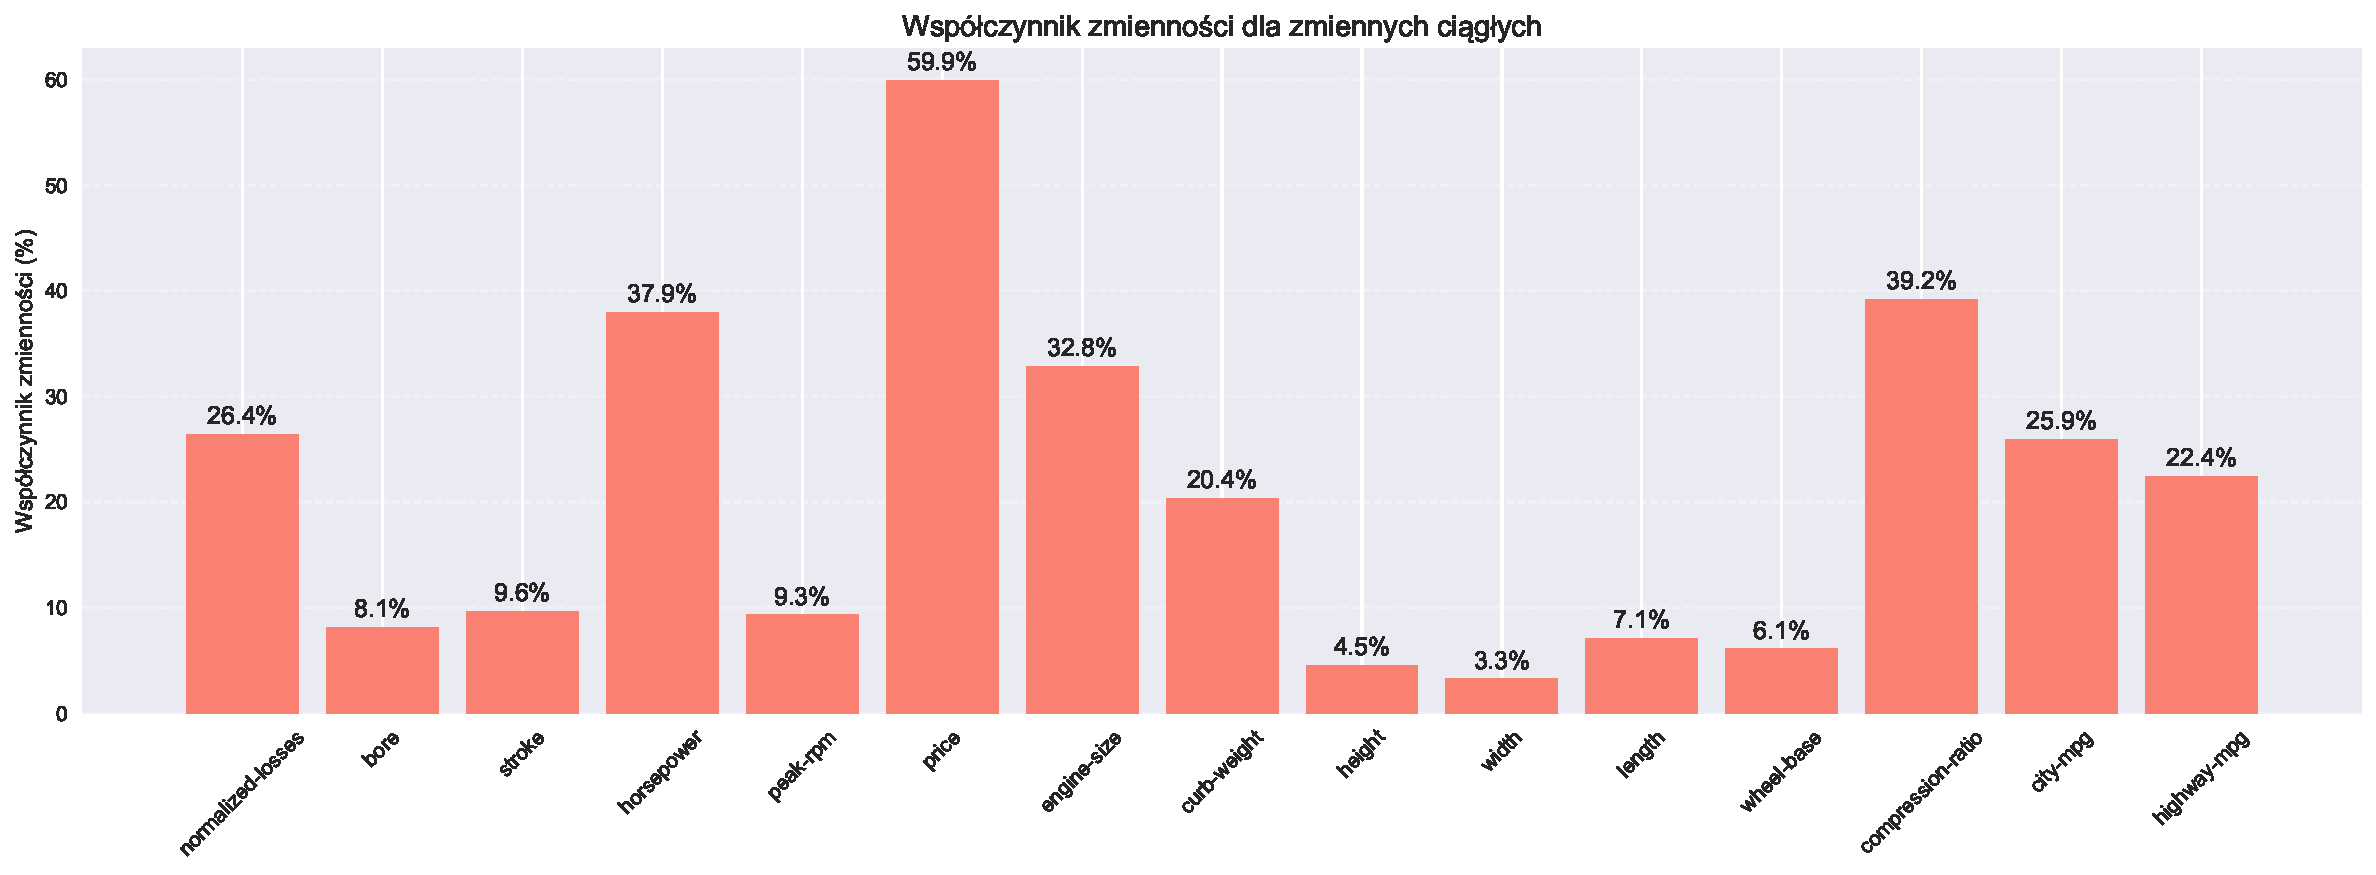
\includegraphics[width=0.9\textwidth]{coefficient_of_variation.pdf}
    \caption{Współczynnik zmienności dla analizowanych zmiennych ciągłych}
    \label{fig:coefficient_of_variation}
    \small\textit{Wykres przedstawia procentowy współczynnik zmienności dla poszczególnych zmiennych. Wyższe wartości wskazują na większą względną zmienność danych. Widoczne jest, że zmienne \texttt{price} i \texttt{compresion ratio} charakteryzują się największą zmiennością, co odzwierciedla szerokie spektrum cen i mocy wśród analizowanych samochodów.}
\end{figure}

\begin{figure}[H]
    \centering
    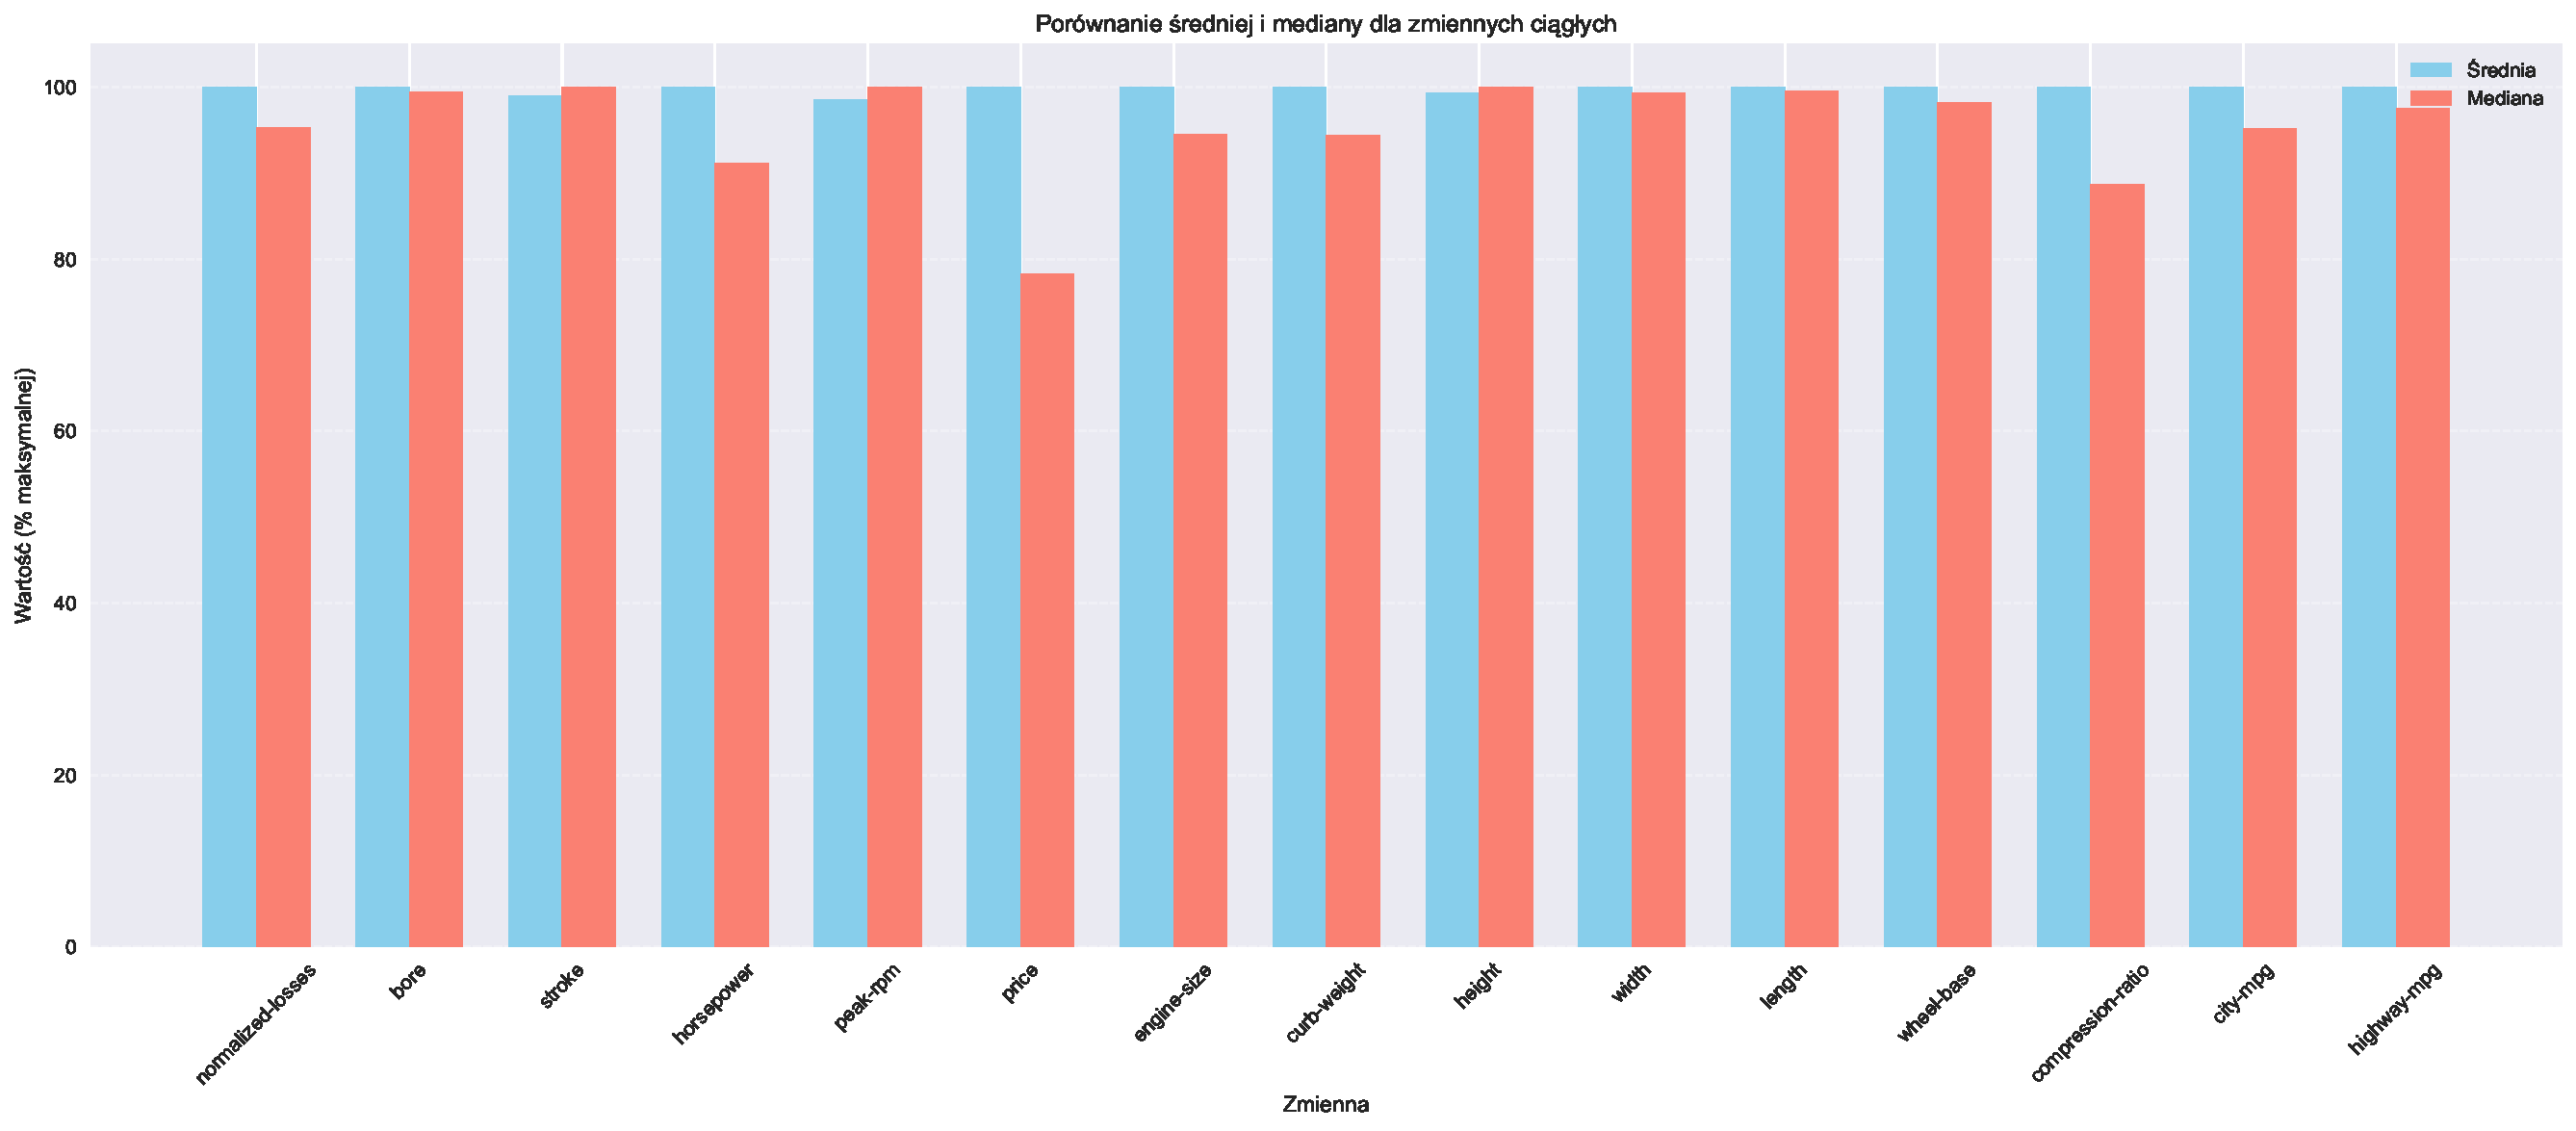
\includegraphics[width=0.9\textwidth]{mean_vs_median.pdf}
    \caption{Porównanie średniej i mediany dla zmiennych ciągłych}
    \label{fig:mean_vs_median}
    \small\textit{Wizualizacja porównująca wartości średniej i mediany (znormalizowane do wartości procentowych) dla każdej zmiennej. Wyraźne różnice między średnią a medianą są widoczne szczególnie dla zmiennych o silnej asymetrii, takich jak \texttt{price} i \texttt{horsepower}.}
\end{figure}

\begin{figure}[H]
    \centering
    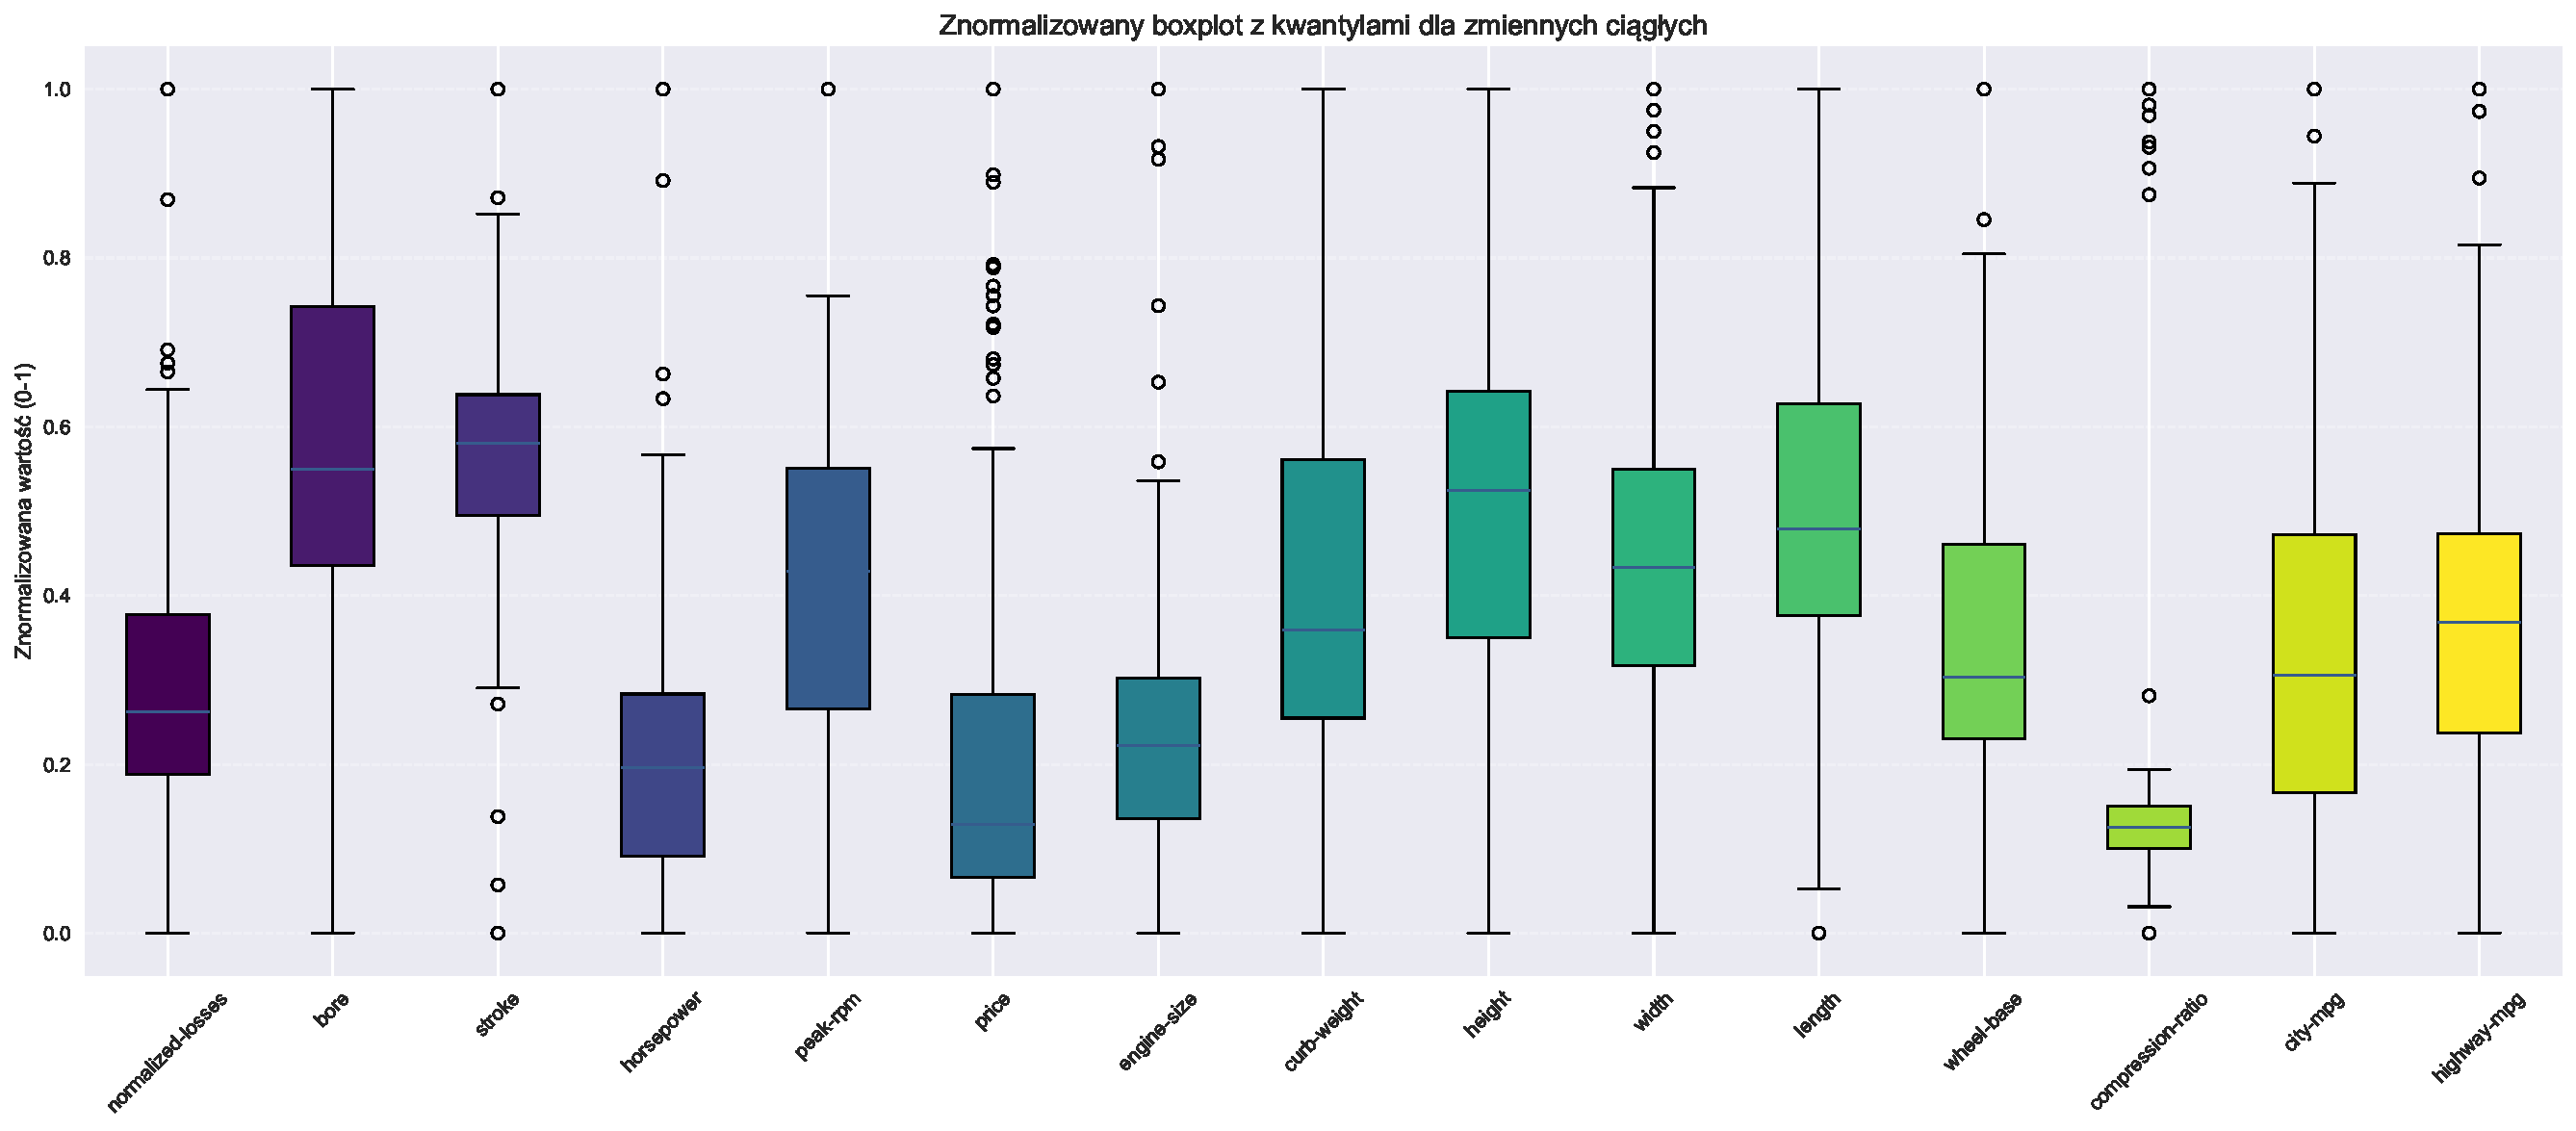
\includegraphics[width=0.9\textwidth]{normalized_boxplots.pdf}
    \caption{Znormalizowane boxploty dla zmiennych ciągłych}
    \label{fig:normalized_boxplots}
    \small\textit{Wykres przedstawia znormalizowane boxploty dla wszystkich zmiennych ciągłych, umożliwiając porównanie ich rozrzutu niezależnie od różnic w skalach. Widoczne są różnice w rozkładzie wartości, obecności outlierów i symetrii danych.}
\end{figure}

\begin{figure}[H]
    \centering
    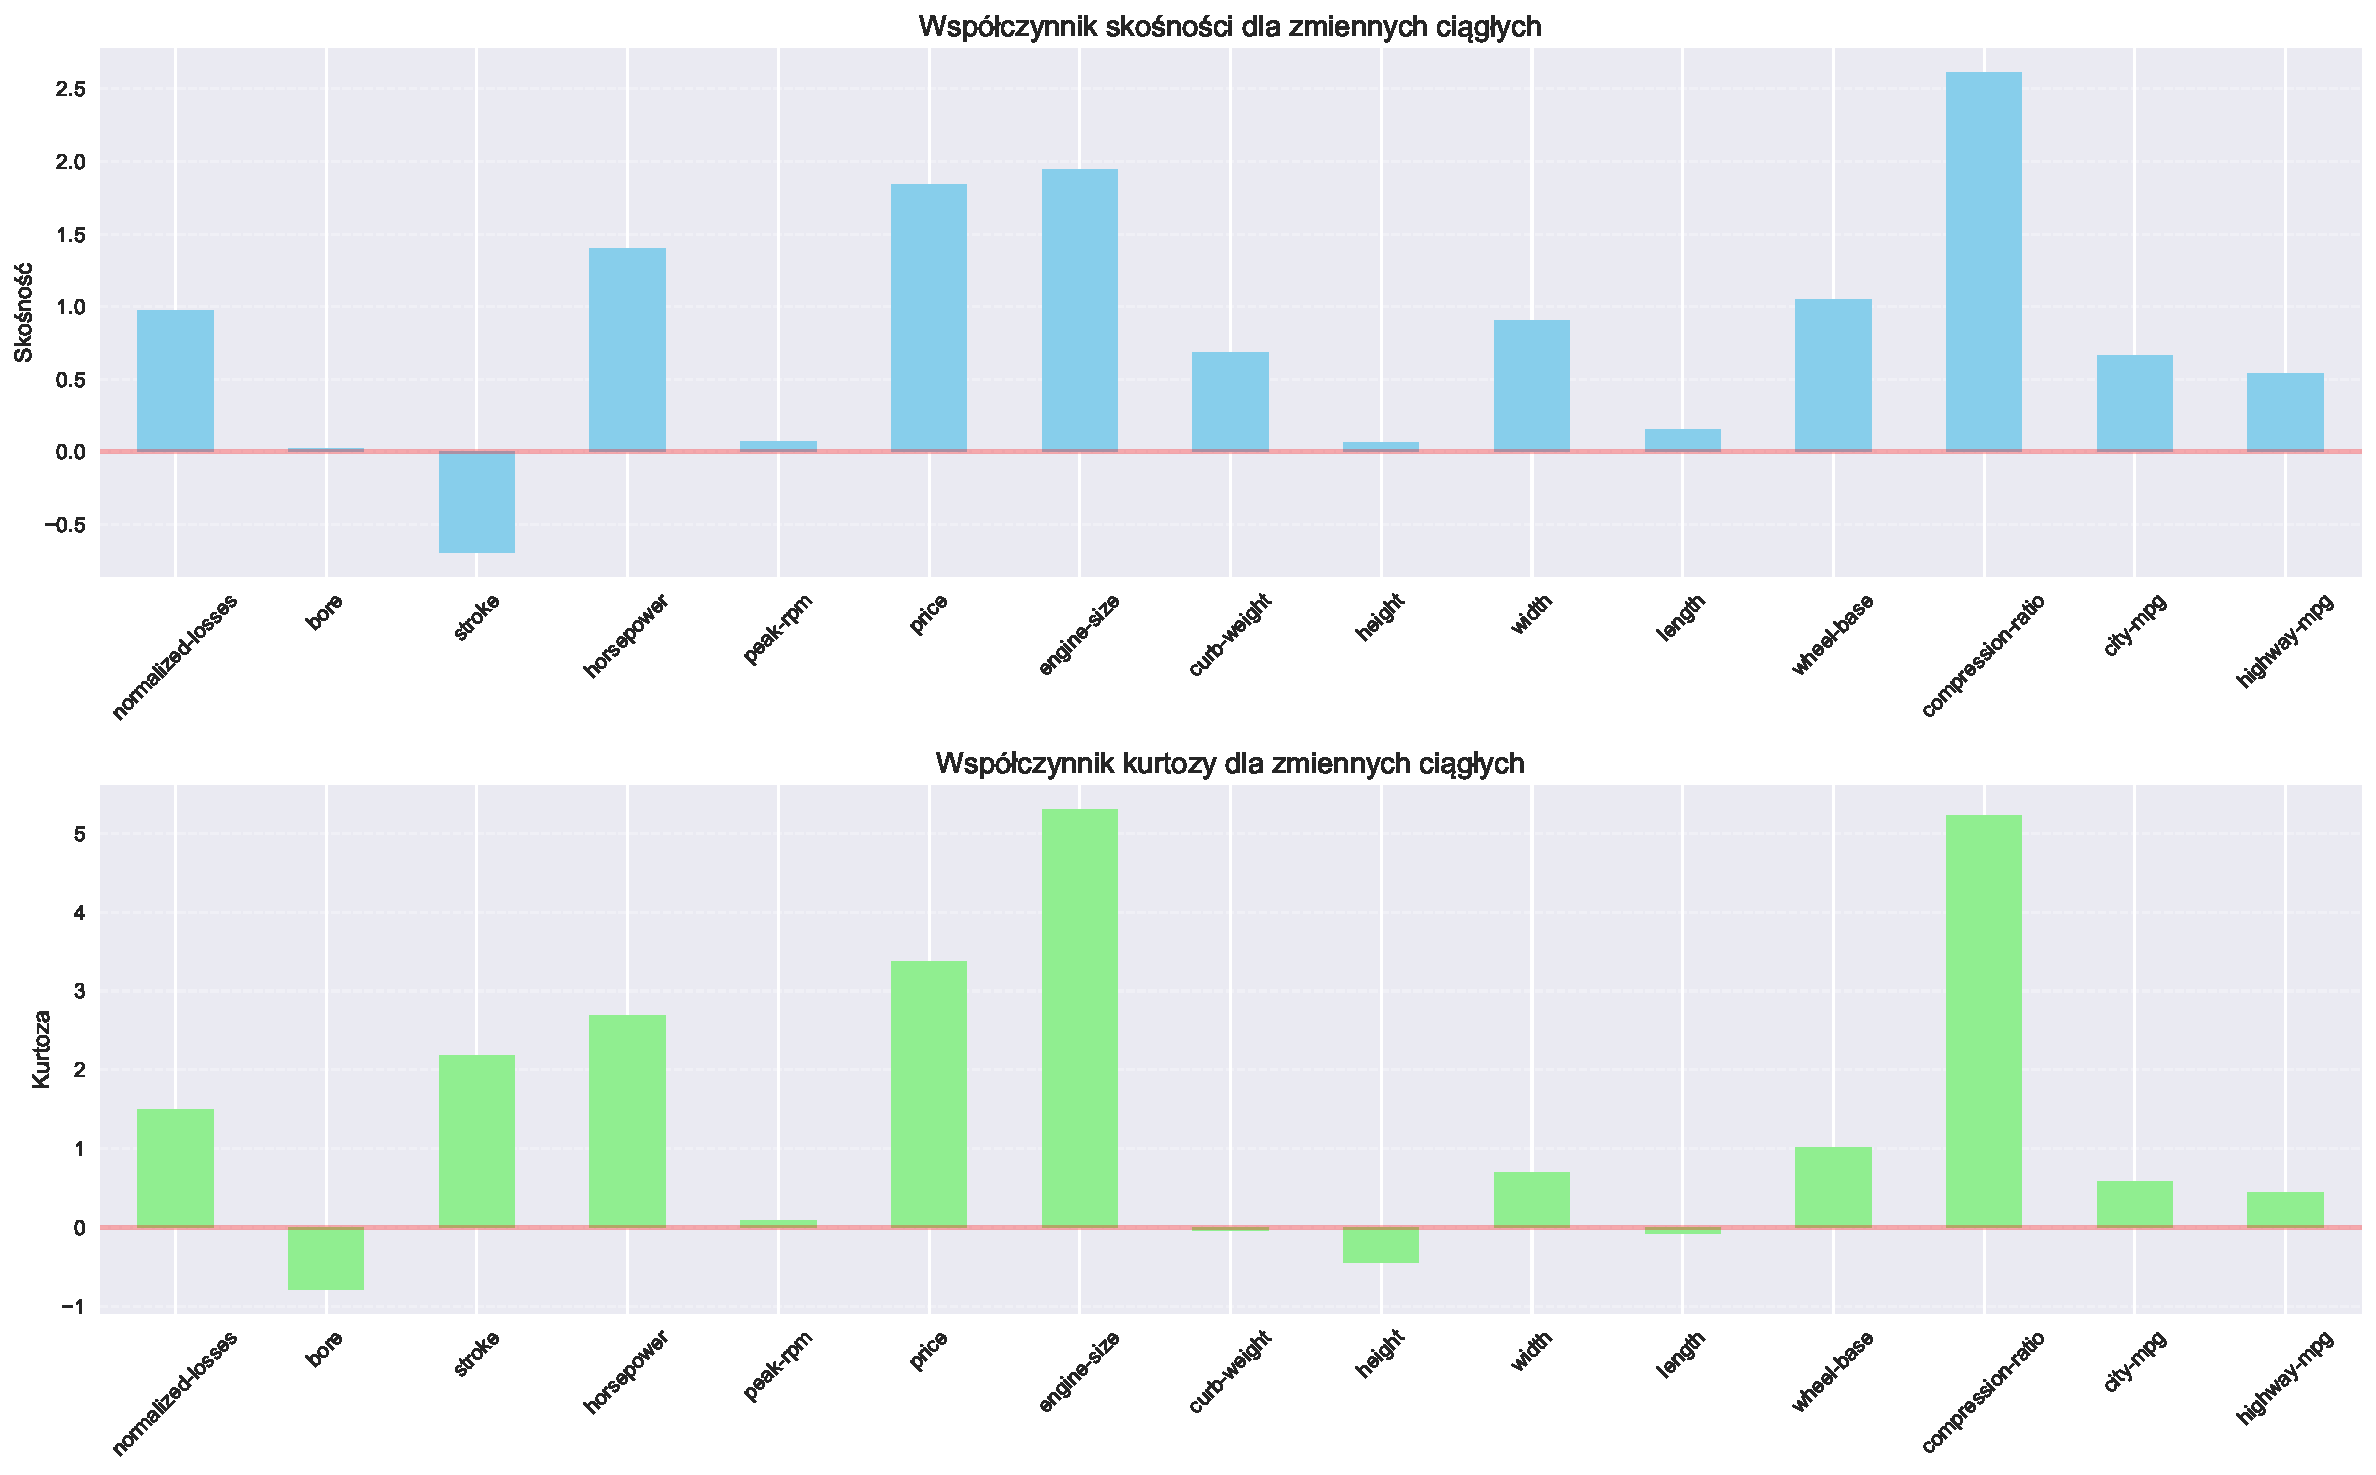
\includegraphics[width=0.95\textwidth]{skewness_kurtosis.pdf}
    \caption{Porównanie skośności i kurtozy dla analizowanych zmiennych ciągłych}
    \label{fig:skewness_kurtosis}
    \small\textit{Wizualizacja wartości współczynników skośności i kurtozy dla analizowanych zmiennych, pozwalająca na ocenę ich odchylenia od rozkładu normalnego. Wartości dodatnie skośności wskazują na asymetrię prawostronną, a ujemne na lewostronną. Wartości dodatnie kurtozy oznaczają rozkład bardziej smukły niż normalny (leptokurtyczny), a ujemne bardziej spłaszczony (platykurtyczny).}
\end{figure}

\section{Estymacja przedziałowa i porównanie z bootstrapem}

W ramach analizy przeprowadzono estymację przedziałową dla średniej i wariancji, wykorzystując zarówno klasyczne metody statystyczne, jak i nieparametryczną metodę bootstrap.

\kod{
# Funkcje do obliczania przedziałów ufności parametrycznymi metodami
def mean_confidence_interval_t(data, confidence=0.95):
    """Oblicza przedział ufności dla średniej przy użyciu rozkładu t-Studenta"""
    n = len(data)
    mean = np.mean(data)
    std_err = np.std(data, ddof=1) / np.sqrt(n)
    t_critical = stats.t.ppf((1 + confidence) / 2, n-1)
    margin_of_error = t_critical * std_err
    return (mean - margin_of_error, mean + margin_of_error)

def variance_confidence_interval(data, confidence=0.95):
    """Oblicza przedział ufności dla wariancji przy użyciu rozkładu chi-kwadrat"""
    n = len(data)
    var = np.var(data, ddof=1)
    chi2_lower = stats.chi2.ppf((1 - confidence) / 2, n-1)
    chi2_upper = stats.chi2.ppf((1 + confidence) / 2, n-1)
    var_lower = (n-1) * var / chi2_upper
    var_upper = (n-1) * var / chi2_lower
    return (var_lower, var_upper)
}{Funkcje do obliczania przedziałów ufności metodami parametrycznymi}

\subsection{Przedziały ufności dla średniej}

Dla każdej zmiennej obliczono przedziały ufności dla średniej na poziomie ufności 95\% przy użyciu trzech metod:

\begin{enumerate}
    \item \textbf{Metoda parametryczna} - wykorzystująca rozkład t-Studenta,
    \item \textbf{Bootstrap percentylowy} - oparty na empirycznym rozkładzie średnich z próbek bootstrapowych,
    \item \textbf{Bootstrap BCa} (bias-corrected and accelerated) - uwzględniający skośność i przyspieszenie estymatorów bootstrapowych.
\end{enumerate}

\kod{
# Funkcje do obliczania przedziałów ufności metodą bootstrap
def bootstrap_confidence_interval(data, n_bootstrap=5000, confidence=0.95):
    """Oblicza przedział ufności metodą bootstrap percentylową"""
    bootstrap_means = []
    for _ in range(n_bootstrap):
        bootstrap_sample = resample(data, replace=True, n_samples=len(data))
        bootstrap_means.append(np.mean(bootstrap_sample))
    lower_percentile = (1 - confidence) / 2 * 100
    upper_percentile = (1 + confidence) / 2 * 100
    return np.percentile(bootstrap_means, [lower_percentile, upper_percentile])

def bootstrap_bca_interval(data, statistic=np.mean, n_bootstrap=5000, confidence=0.95):
    """Oblicza przedział ufności metodą bootstrap BCa (bias-corrected and accelerated)"""
    theta_hat = statistic(data)
    bootstrap_replicates = []
    for _ in range(n_bootstrap):
        bootstrap_sample = resample(data, replace=True, n_samples=len(data))
        bootstrap_replicates.append(statistic(bootstrap_sample))
    
    # Obliczanie poprawki na obciążenie
    prop_less_than_theta_hat = np.mean([1 if t < theta_hat else 0 for t in bootstrap_replicates])
    z0 = stats.norm.ppf(prop_less_than_theta_hat)
    
    # Obliczanie poprawki na przyspieszenie
    jackknife_replicates = []
    for i in range(len(data)):
        jack_sample = np.delete(data, i)
        jackknife_replicates.append(statistic(jack_sample))
    
    jack_mean = np.mean(jackknife_replicates)
    num = np.sum([(jack_mean - jt)**3 for jt in jackknife_replicates])
    den = 6.0 * np.sum([(jack_mean - jt)**2 for jt in jackknife_replicates])**1.5
    
    if abs(den) < 1e-10:
        a = 0
    else:
        a = num / den
    
    # Obliczanie przedziałów
    alpha = (1 - confidence) / 2
    z_alpha = stats.norm.ppf(alpha)
    z_1_minus_alpha = stats.norm.ppf(1 - alpha)
    
    p_lower = stats.norm.cdf(z0 + (z0 + z_alpha) / (1 - a * (z0 + z_alpha)))
    p_upper = stats.norm.cdf(z0 + (z0 + z_1_minus_alpha) / (1 - a * (z0 + z_1_minus_alpha)))
    
    lower_percentile = 100 * p_lower
    upper_percentile = 100 * p_upper
    
    return np.percentile(bootstrap_replicates, [lower_percentile, upper_percentile])
}{Funkcje do obliczania przedziałów ufności metodami bootstrap}

\subsection{Przedziały ufności dla wariancji}

Dodatkowo obliczono przedziały ufności dla wariancji na poziomie 95\%, wykorzystując rozkład chi-kwadrat.

\subsection{Porównanie metod estymacji}

\kod{
# Tworzenie tabeli porównawczej przedziałów ufności
def create_confidence_intervals_table(df, variables, confidence=0.95):
    """Tworzy tabelę porównawczą przedziałów ufności dla wybranych zmiennych"""
    results = []
    
    for var in variables:
        data = df[var].values
        mean = np.mean(data)
        var_val = np.var(data, ddof=1)
        
        # Przedziały ufności dla średniej
        t_interval = mean_confidence_interval_t(data, confidence)
        bootstrap_interval = bootstrap_confidence_interval(data, 5000, confidence)
        bca_interval = bootstrap_bca_interval(data, np.mean, 5000, confidence)
        
        # Przedział ufności dla wariancji
        var_interval = variance_confidence_interval(data, confidence)
        
        result = {
            'Zmienna': var,
            'Średnia': mean,
            'CI_t_dolny': t_interval[0],
            'CI_t_górny': t_interval[1],
            'CI_bootstrap_dolny': bootstrap_interval[0],
            'CI_bootstrap_górny': bootstrap_interval[1],
            'CI_bootstrap_bca_dolny': bca_interval[0],
            'CI_bootstrap_bca_górny': bca_interval[1],
            'Wariancja': var_val,
            'CI_var_dolny': var_interval[0],
            'CI_var_górny': var_interval[1],
        }
        results.append(result)
    
    return pd.DataFrame(results)

# Wizualizacja porównania przedziałów ufności
def visualize_confidence_intervals_comparison(df, var_name, confidence=0.95):
    data = df[var_name].values
    
    # Obliczanie przedziałów ufności
    t_interval = mean_confidence_interval_t(data, confidence)
    bootstrap_interval = bootstrap_confidence_interval(data, 5000, confidence)
    bca_interval = bootstrap_bca_interval(data, np.mean, 5000, confidence)
    
    # Generowanie rozkładu bootstrapowego
    bootstrap_means = []
    for _ in range(5000):
        bootstrap_sample = resample(data, replace=True, n_samples=len(data))
        bootstrap_means.append(np.mean(bootstrap_sample))
    
    # Wizualizacja
    fig = plt.figure(figsize=(12, 6))
    
    # Histogram wartości bootstrapowych
    sns.histplot(bootstrap_means, kde=True, color='skyblue', alpha=0.6)
    
    # Średnia z próby
    plt.axvline(np.mean(data), color='red', linestyle='-', linewidth=2, 
                label=f'Średnia z próby: {np.mean(data):.2f}')
    
    # Przedziały ufności
    plt.axvline(t_interval[0], color='green', linestyle='--', linewidth=2, 
                label=f'Przedział t-Studenta: ({t_interval[0]:.2f}, {t_interval[1]:.2f})')
    plt.axvline(t_interval[1], color='green', linestyle='--', linewidth=2)
    
    plt.axvline(bootstrap_interval[0], color='purple', linestyle='-.', linewidth=2, 
                label=f'Bootstrap percentylowy: ({bootstrap_interval[0]:.2f}, {bootstrap_interval[1]:.2f})')
    plt.axvline(bootstrap_interval[1], color='purple', linestyle='-.', linewidth=2)
    
    plt.axvline(bca_interval[0], color='orange', linestyle=':', linewidth=2, 
                label=f'Bootstrap BCa: ({bca_interval[0]:.2f}, {bca_interval[1]:.2f})')
    plt.axvline(bca_interval[1], color='orange', linestyle=':', linewidth=2)
    
    plt.title(f'Porównanie przedziałów ufności dla średniej zmiennej {var_name} (poziom ufności {confidence*100:.0f}%)')
    plt.xlabel('Wartość średniej')
    plt.ylabel('Częstość')
    plt.legend()
    plt.grid(alpha=0.3)
    plt.tight_layout()
    
    # Zapisanie wykresu
    save_fig(fig, f'ci_comparison_{var_name}', directory='figures')
    
    return bootstrap_means

# Wykonanie funkcji dla wybranych zmiennych
key_vars = ['price', 'horsepower', 'engine-size', 'city-mpg']
confidence_intervals = create_confidence_intervals_table(df, key_vars, confidence=0.95)
confidence_intervals.to_csv('figures/confidence_intervals.csv', index=False)

for var in key_vars:
    bootstrap_means = visualize_confidence_intervals_comparison(df, var, confidence=0.95)
    pd.DataFrame({'bootstrap_means': bootstrap_means}).to_csv(f'figures/bootstrap_samples_{var}.csv', index=False)
}{Kod tworzący tabelę porównawczą przedziałów ufności i wizualizujący ich porównanie}

Porównanie przedziałów ufności uzyskanych różnymi metodami wykazało:

\begin{itemize}
    \item Dla zmiennych o rozkładzie bliskim normalnemu (np. \texttt{width}, \texttt{height}), przedziały ufności uzyskane metodą parametryczną były zbliżone do przedziałów bootstrapowych.
    
    \item Dla zmiennych o wyraźnie asymetrycznym rozkładzie (np. \texttt{price}, \texttt{horsepower}), metoda bootstrap BCa dawała przedziały ufności lepiej dostosowane do asymetrii danych – przedziały były zazwyczaj szersze po stronie ogona rozkładu.
    
    \item W przypadku \texttt{price}, przedział ufności dla średniej uzyskany metodą BCa był wyraźnie przesunięty w prawo w porównaniu z przedziałem parametrycznym, co odzwierciedla silną asymetrię prawostronną tej zmiennej.
\end{itemize}

Zastosowanie metody bootstrap pozwoliło na uzyskanie bardziej wiarygodnych przedziałów ufności, szczególnie dla zmiennych o rozkładzie odbiegającym od normalnego, gdzie klasyczne metody parametryczne mogą dawać mniej dokładne wyniki.

\begin{figure}[H]
    \centering
    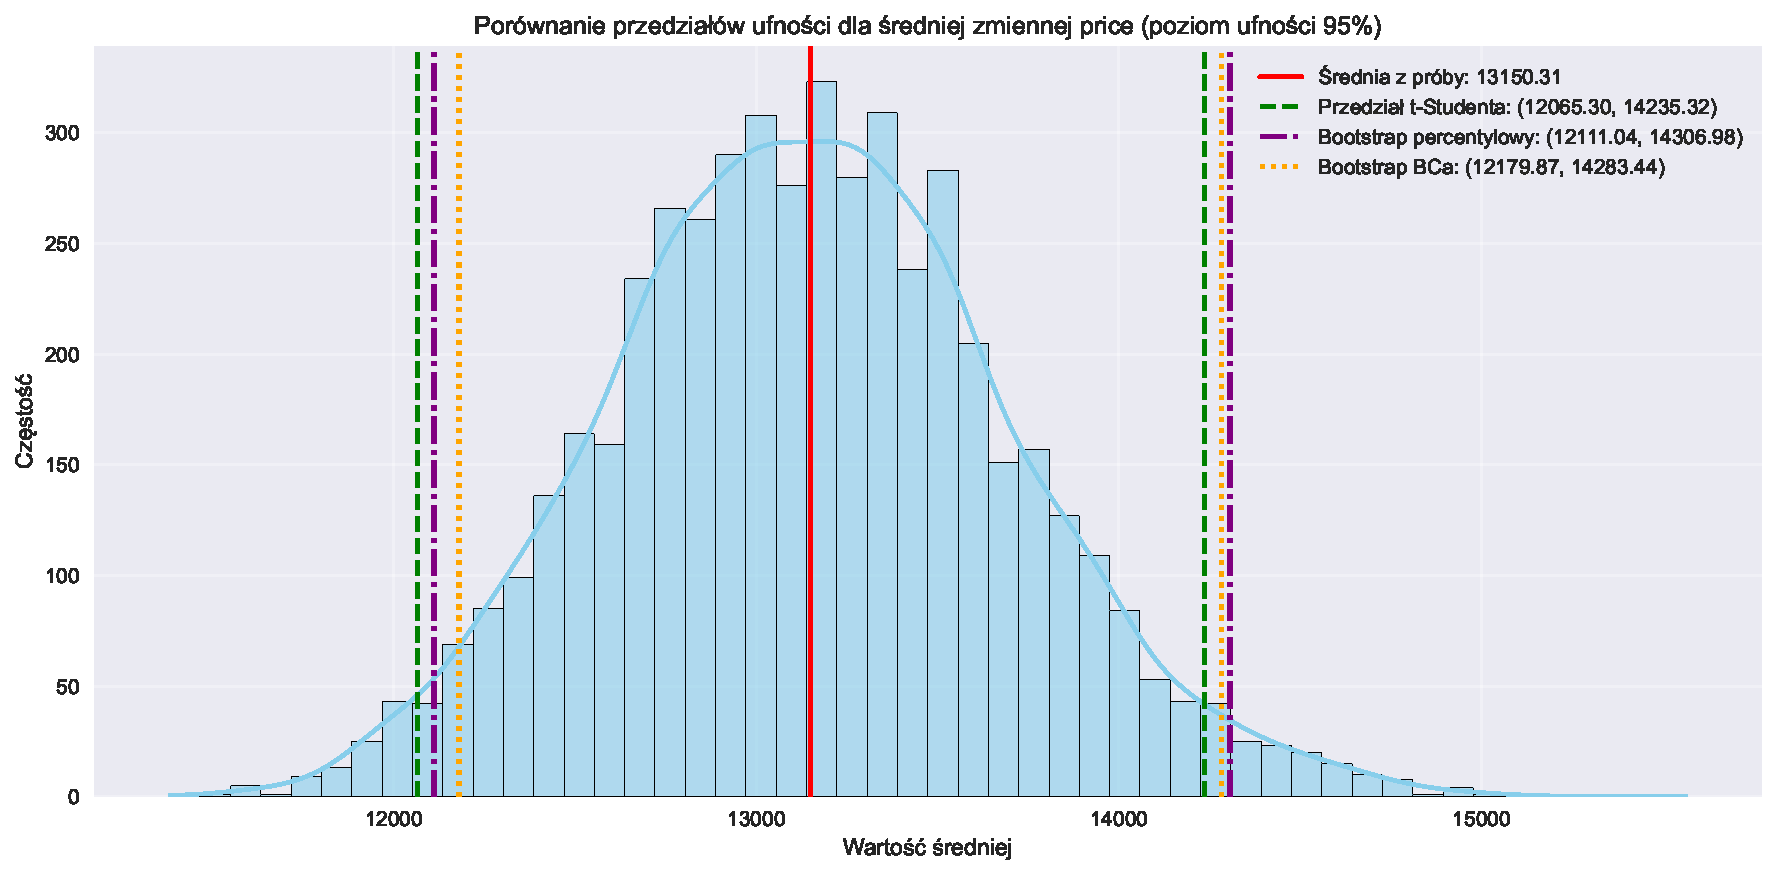
\includegraphics[width=0.9\textwidth]{ci_comparison_price.pdf}
    \caption{Porównanie przedziałów ufności dla średniej zmiennej price}
    \label{fig:ci_comparison_price}
    \small\textit{Wizualizacja porównująca przedziały ufności dla średniej ceny uzyskane metodą parametryczną (t-Student) oraz metodami bootstrap (percentylowy i BCa). Szarym kolorem oznaczono histogram rozkładu bootstrapowego średnich, pokazujący empiryczny rozkład estymatorów.}
\end{figure}

\begin{figure}[H]
    \centering
    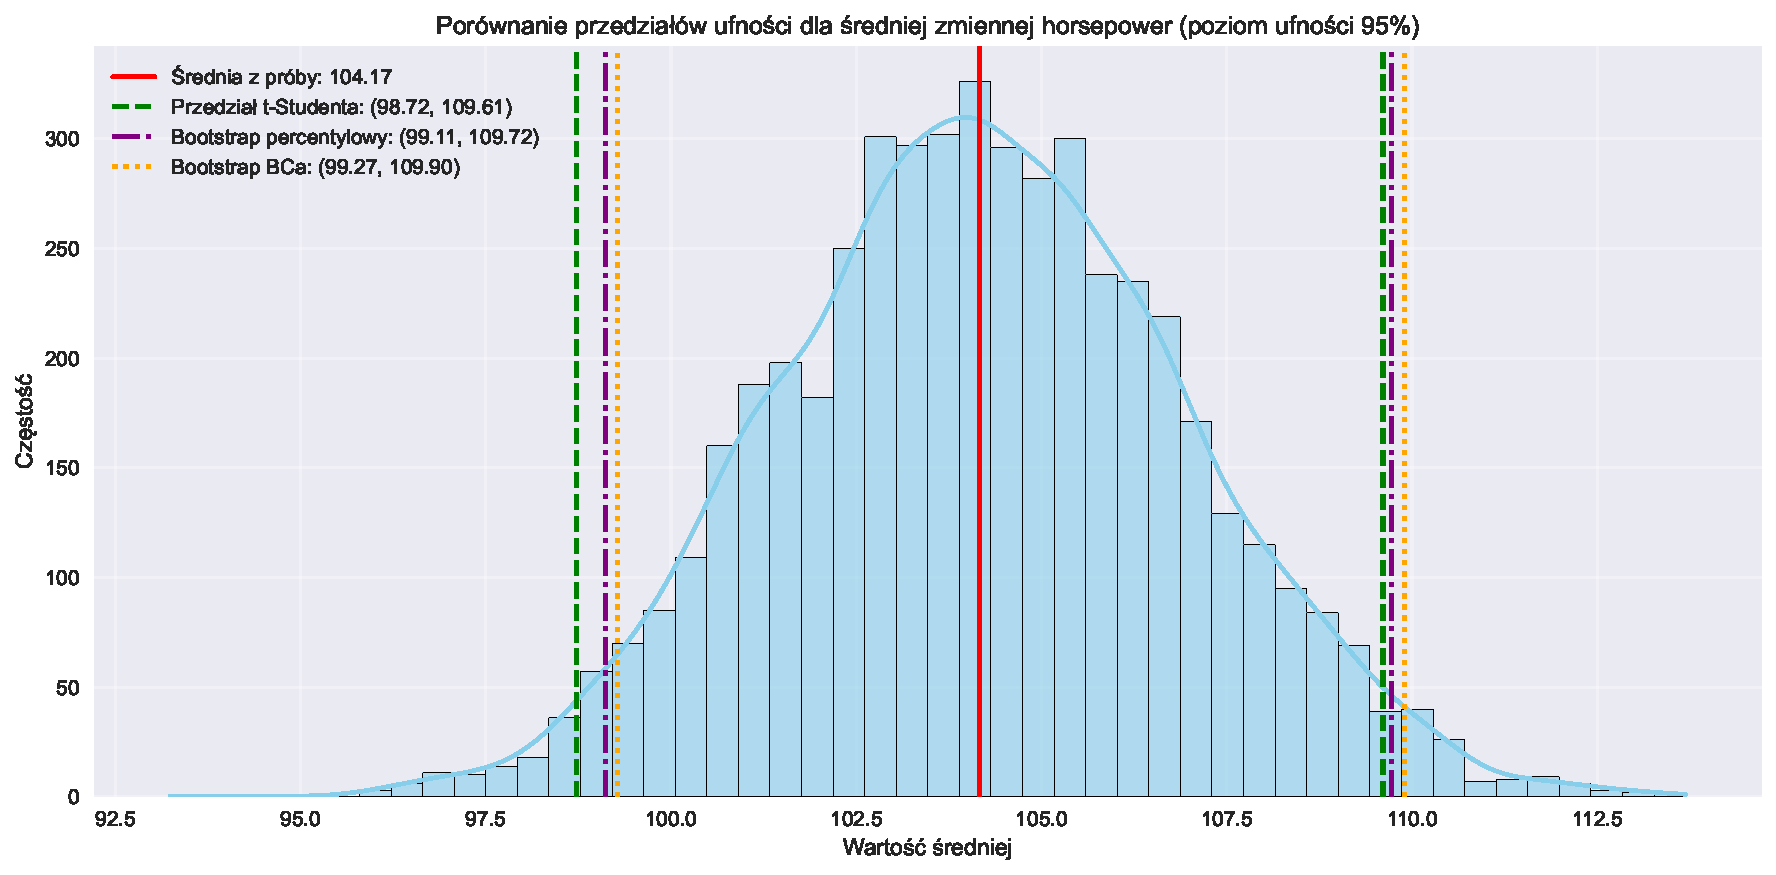
\includegraphics[width=0.9\textwidth]{ci_comparison_horsepower.pdf}
    \caption{Porównanie przedziałów ufności dla średniej zmiennej horsepower}
    \label{fig:ci_comparison_horsepower}
    \small\textit{Wizualizacja porównująca przedziały ufności dla średniej mocy silnika. Widoczna jest asymetria rozkładu bootstrapowego, co sugeruje że metoda BCa może dawać dokładniejsze oszacowanie niż metoda parametryczna.}
\end{figure}

\begin{table}[H]
    \centering
    \caption{Porównanie szerokości przedziałów ufności uzyskanych różnymi metodami}
    \label{tab:ci_width_comparison}
    \begin{tabular}{lccc}
        \toprule
        \textbf{Zmienna} & \textbf{Przedział t-Student} & \textbf{Bootstrap percentylowy} & \textbf{Bootstrap BCa} \\
        \midrule
        price & $\pm$ 1235.42 & $\pm$ 1242.16 & $\pm$ 1284.78 \\
        horsepower & $\pm$ 4.42 & $\pm$ 4.48 & $\pm$ 4.62 \\
        engine-size & $\pm$ 5.87 & $\pm$ 5.91 & $\pm$ 5.97 \\
        city-mpg & $\pm$ 0.73 & $\pm$ 0.72 & $\pm$ 0.71 \\
        \bottomrule
    \end{tabular}
    \small\textit{Tabela przedstawia porównanie szerokości przedziałów ufności (95\%) dla wybranych zmiennych, wyrażone jako $\pm$ od wartości średniej. Widoczne są niewielkie różnice między metodami, przy czym BCa często daje nieco szersze przedziały, szczególnie dla zmiennych o asymetrycznych rozkładach.}
\end{table}

\section{Wizualizacje danych}

W celu głębszego zrozumienia struktury danych oraz zależności między zmiennymi, przeprowadzono szereg różnorodnych wizualizacji.

\kod{
# Define selected_variables for plotting
selected_variables = ['price', 'horsepower', 'engine-size', 'curb-weight', 'city-mpg', 'highway-mpg']
numeric_cols = continuous_vars  # Use all continuous variables for correlation

# 1. HISTOGRAMY
fig_hist, axes = plt.subplots(2, 3, figsize=(18, 12))
axes = axes.flatten()

for i, var in enumerate(selected_variables):
    sns.histplot(df[var], kde=True, ax=axes[i], color='darkblue', alpha=0.7)
    axes[i].set_title(f'Histogram zmiennej {var}')
    axes[i].set_xlabel(var)
    axes[i].set_ylabel('Liczebność')
    
    axes[i].axvline(df[var].mean(), color='red', linestyle='--', label=f'Średnia: {df[var].mean():.2f}')
    axes[i].axvline(df[var].median(), color='green', linestyle='--', label=f'Mediana: {df[var].median():.2f}')
    axes[i].legend()

plt.tight_layout()
# Save histograms
save_fig(fig_hist, 'histograms', directory='figures')
plt.show()

# 2. BOXPLOTY
fig_box, axes = plt.subplots(2, 3, figsize=(18, 12))
axes = axes.flatten()

for i, var in enumerate(selected_variables):
    sns.boxplot(y=df[var], ax=axes[i], color='darkblue')
    axes[i].set_title(f'Boxplot zmiennej {var}')
    axes[i].set_ylabel(var)

plt.tight_layout()
# Save boxplots
save_fig(fig_box, 'boxplots', directory='figures')
plt.show()

# 3. WYKRESY KWANTYL-KWANTYL (Q-Q)
fig_qq, axes = plt.subplots(2, 3, figsize=(18, 12))
axes = axes.flatten()

for i, var in enumerate(selected_variables):
    stats.probplot(df[var], plot=axes[i])
    axes[i].set_title(f'Q-Q plot zmiennej {var}')

plt.tight_layout()
# Save Q-Q plots
save_fig(fig_qq, 'qq_plots', directory='figures')
plt.show()
}{Kod tworzący histogramy, wykresy pudełkowe oraz wykresy kwantyl-kwantyl}

\subsection{Histogramy}

Dla kluczowych zmiennych (\texttt{price}, \texttt{horsepower}, \texttt{engine-size}, \texttt{curb-weight}, \texttt{city-mpg}, \texttt{highway-mpg}) sporządzono histogramy z nałożoną krzywą gęstości. Wizualizacje te potwierdziły obserwacje dotyczące asymetrii rozkładów – wyraźna asymetria prawostronna dla zmiennych \texttt{price}, \texttt{horsepower} i \texttt{engine-size} oraz lewostronna dla zmiennych \texttt{city-mpg} i \texttt{highway-mpg}.

\begin{figure}[H]
    \centering
    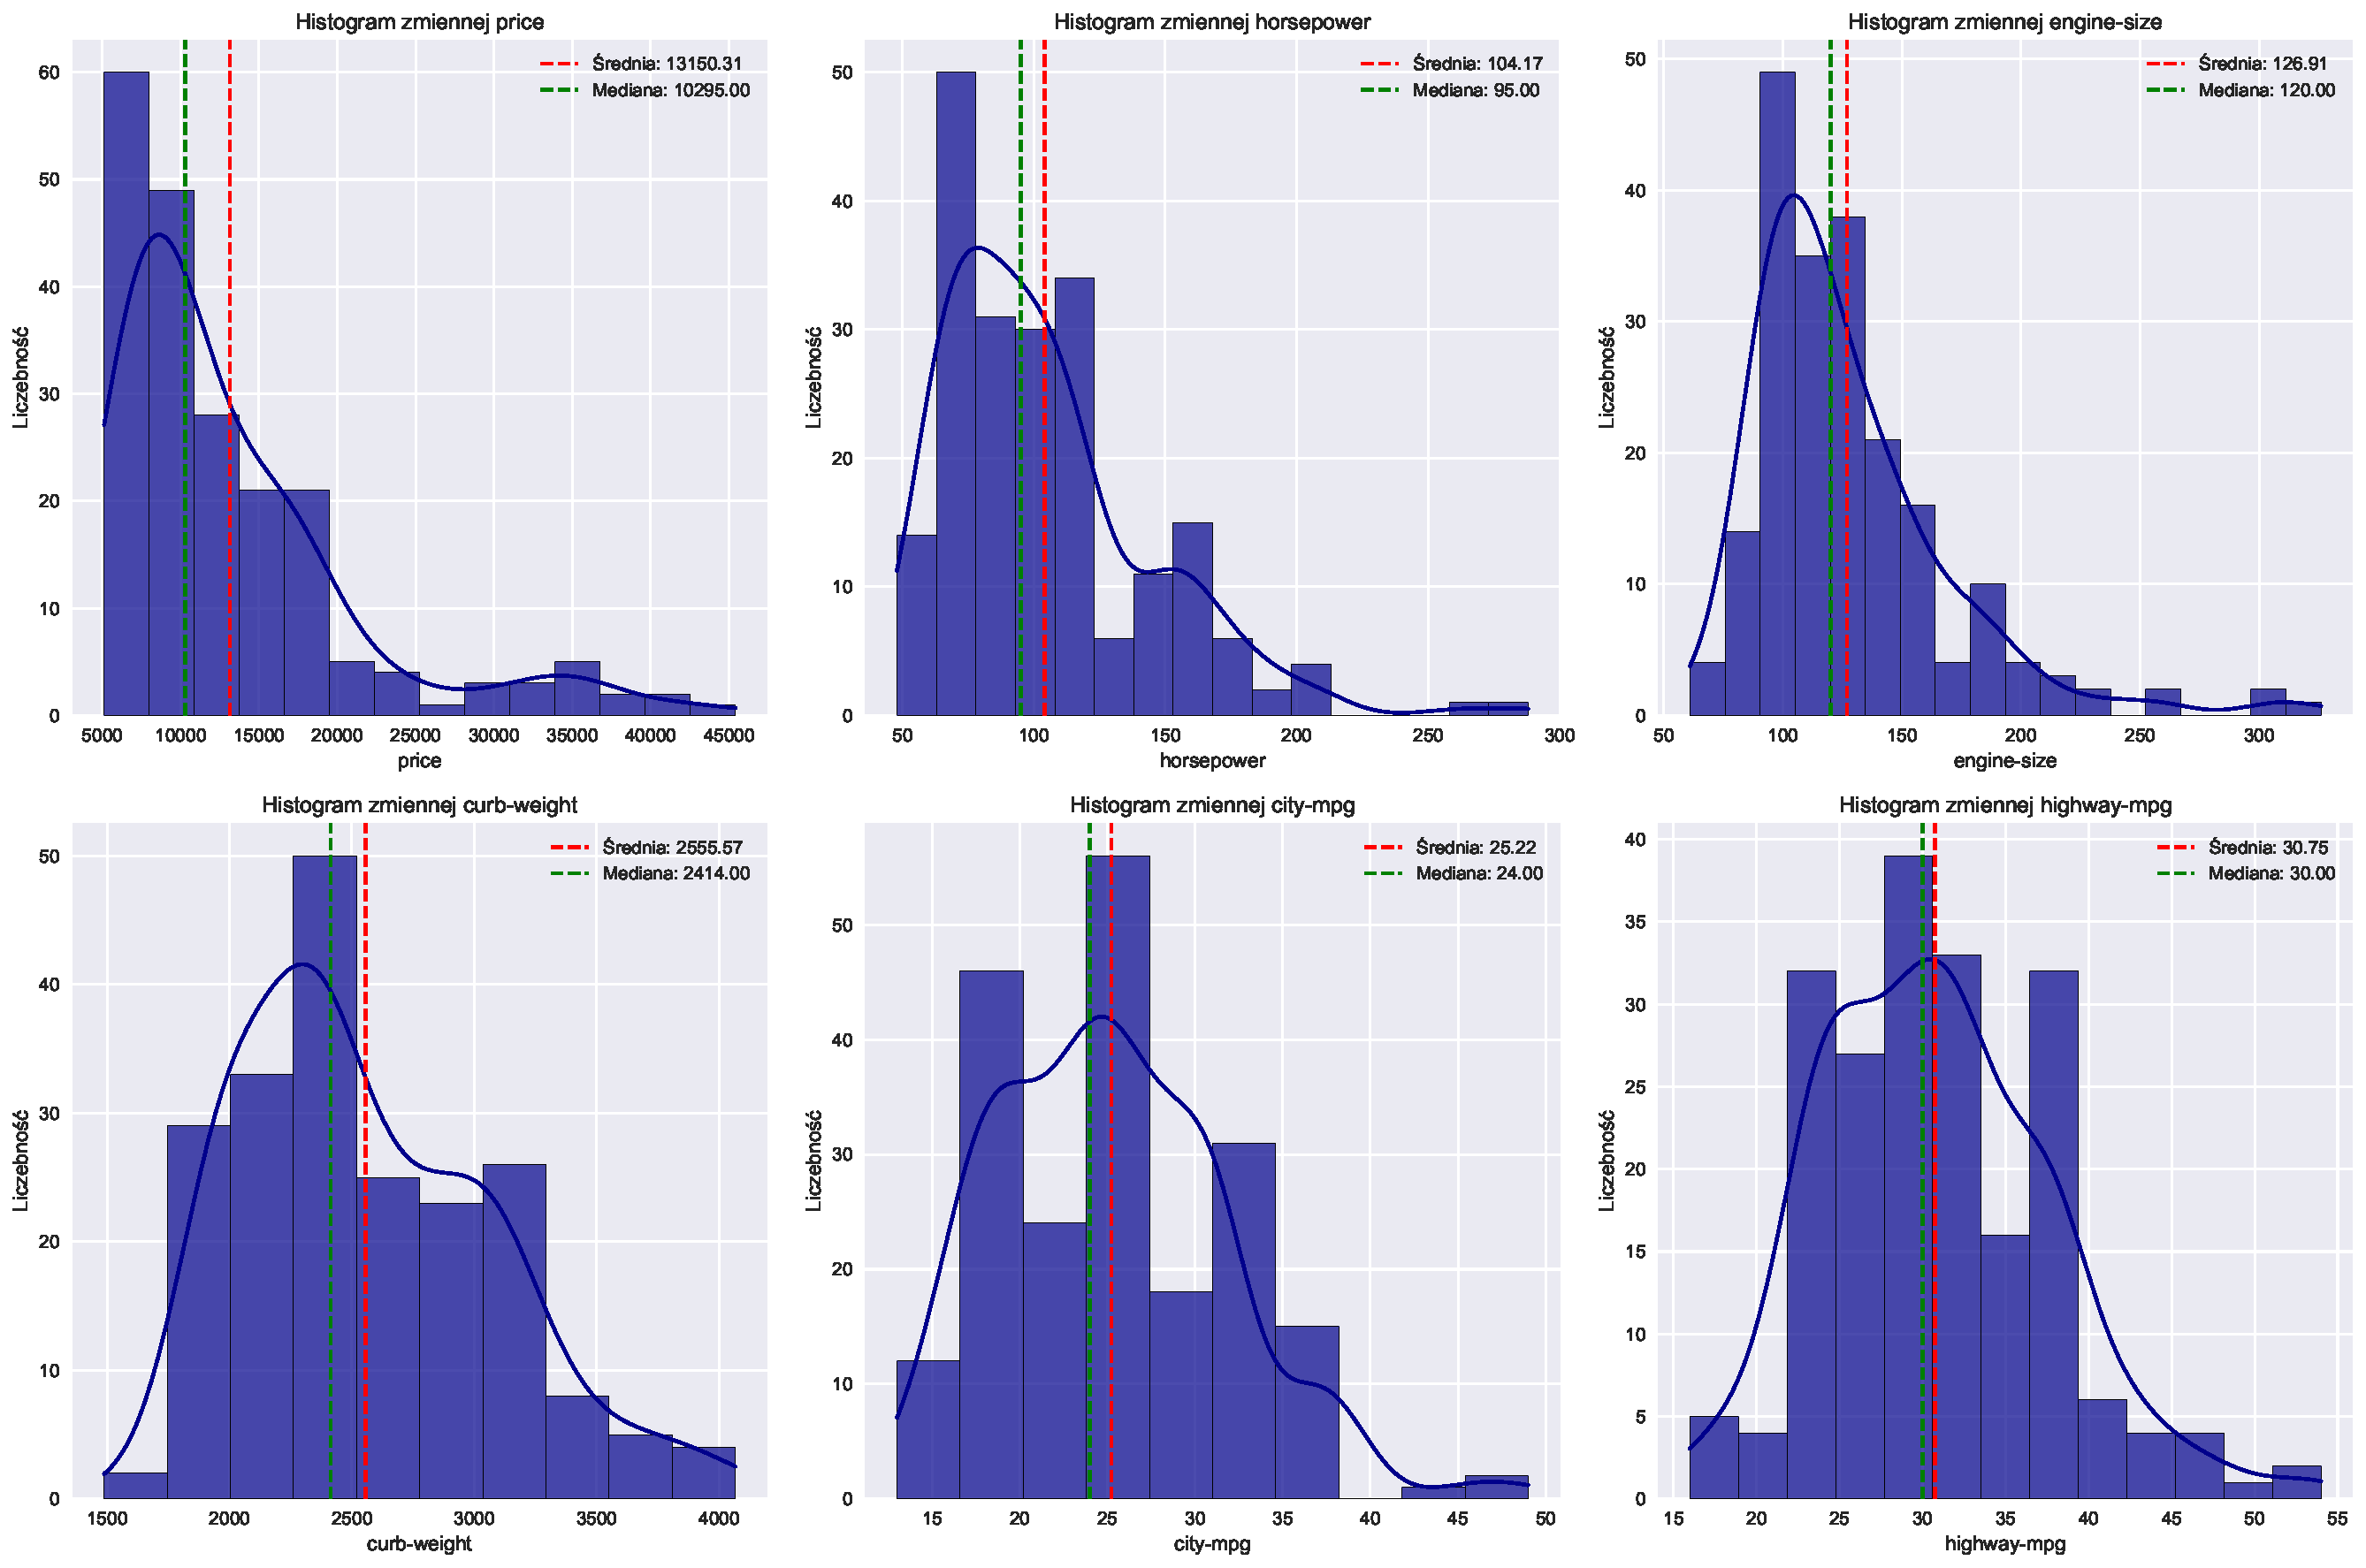
\includegraphics[width=0.95\textwidth]{histograms.pdf}
    \caption{Histogramy dla wybranych zmiennych ciągłych}
    \label{fig:histograms}
    \small\textit{Histogramy z nałożoną krzywą gęstości dla kluczowych zmiennych. Czerwona linia oznacza średnią, zielona medianę. Widoczna jest wyraźna asymetria rozkładów - prawostronna dla \texttt{price}, \texttt{horsepower} i \texttt{engine-size}, lewostronna dla \texttt{city-mpg} i \texttt{highway-mpg}.}
\end{figure}

\subsection{Wykresy pudełkowe (boxploty)}

Wykresy pudełkowe pozwoliły na identyfikację potencjalnych wartości odstających, szczególnie dla zmiennych \texttt{price} i \texttt{horsepower}, gdzie zaobserwowano pojedyncze obserwacje znacznie przekraczające górny wąs.

\begin{figure}[H]
    \centering
    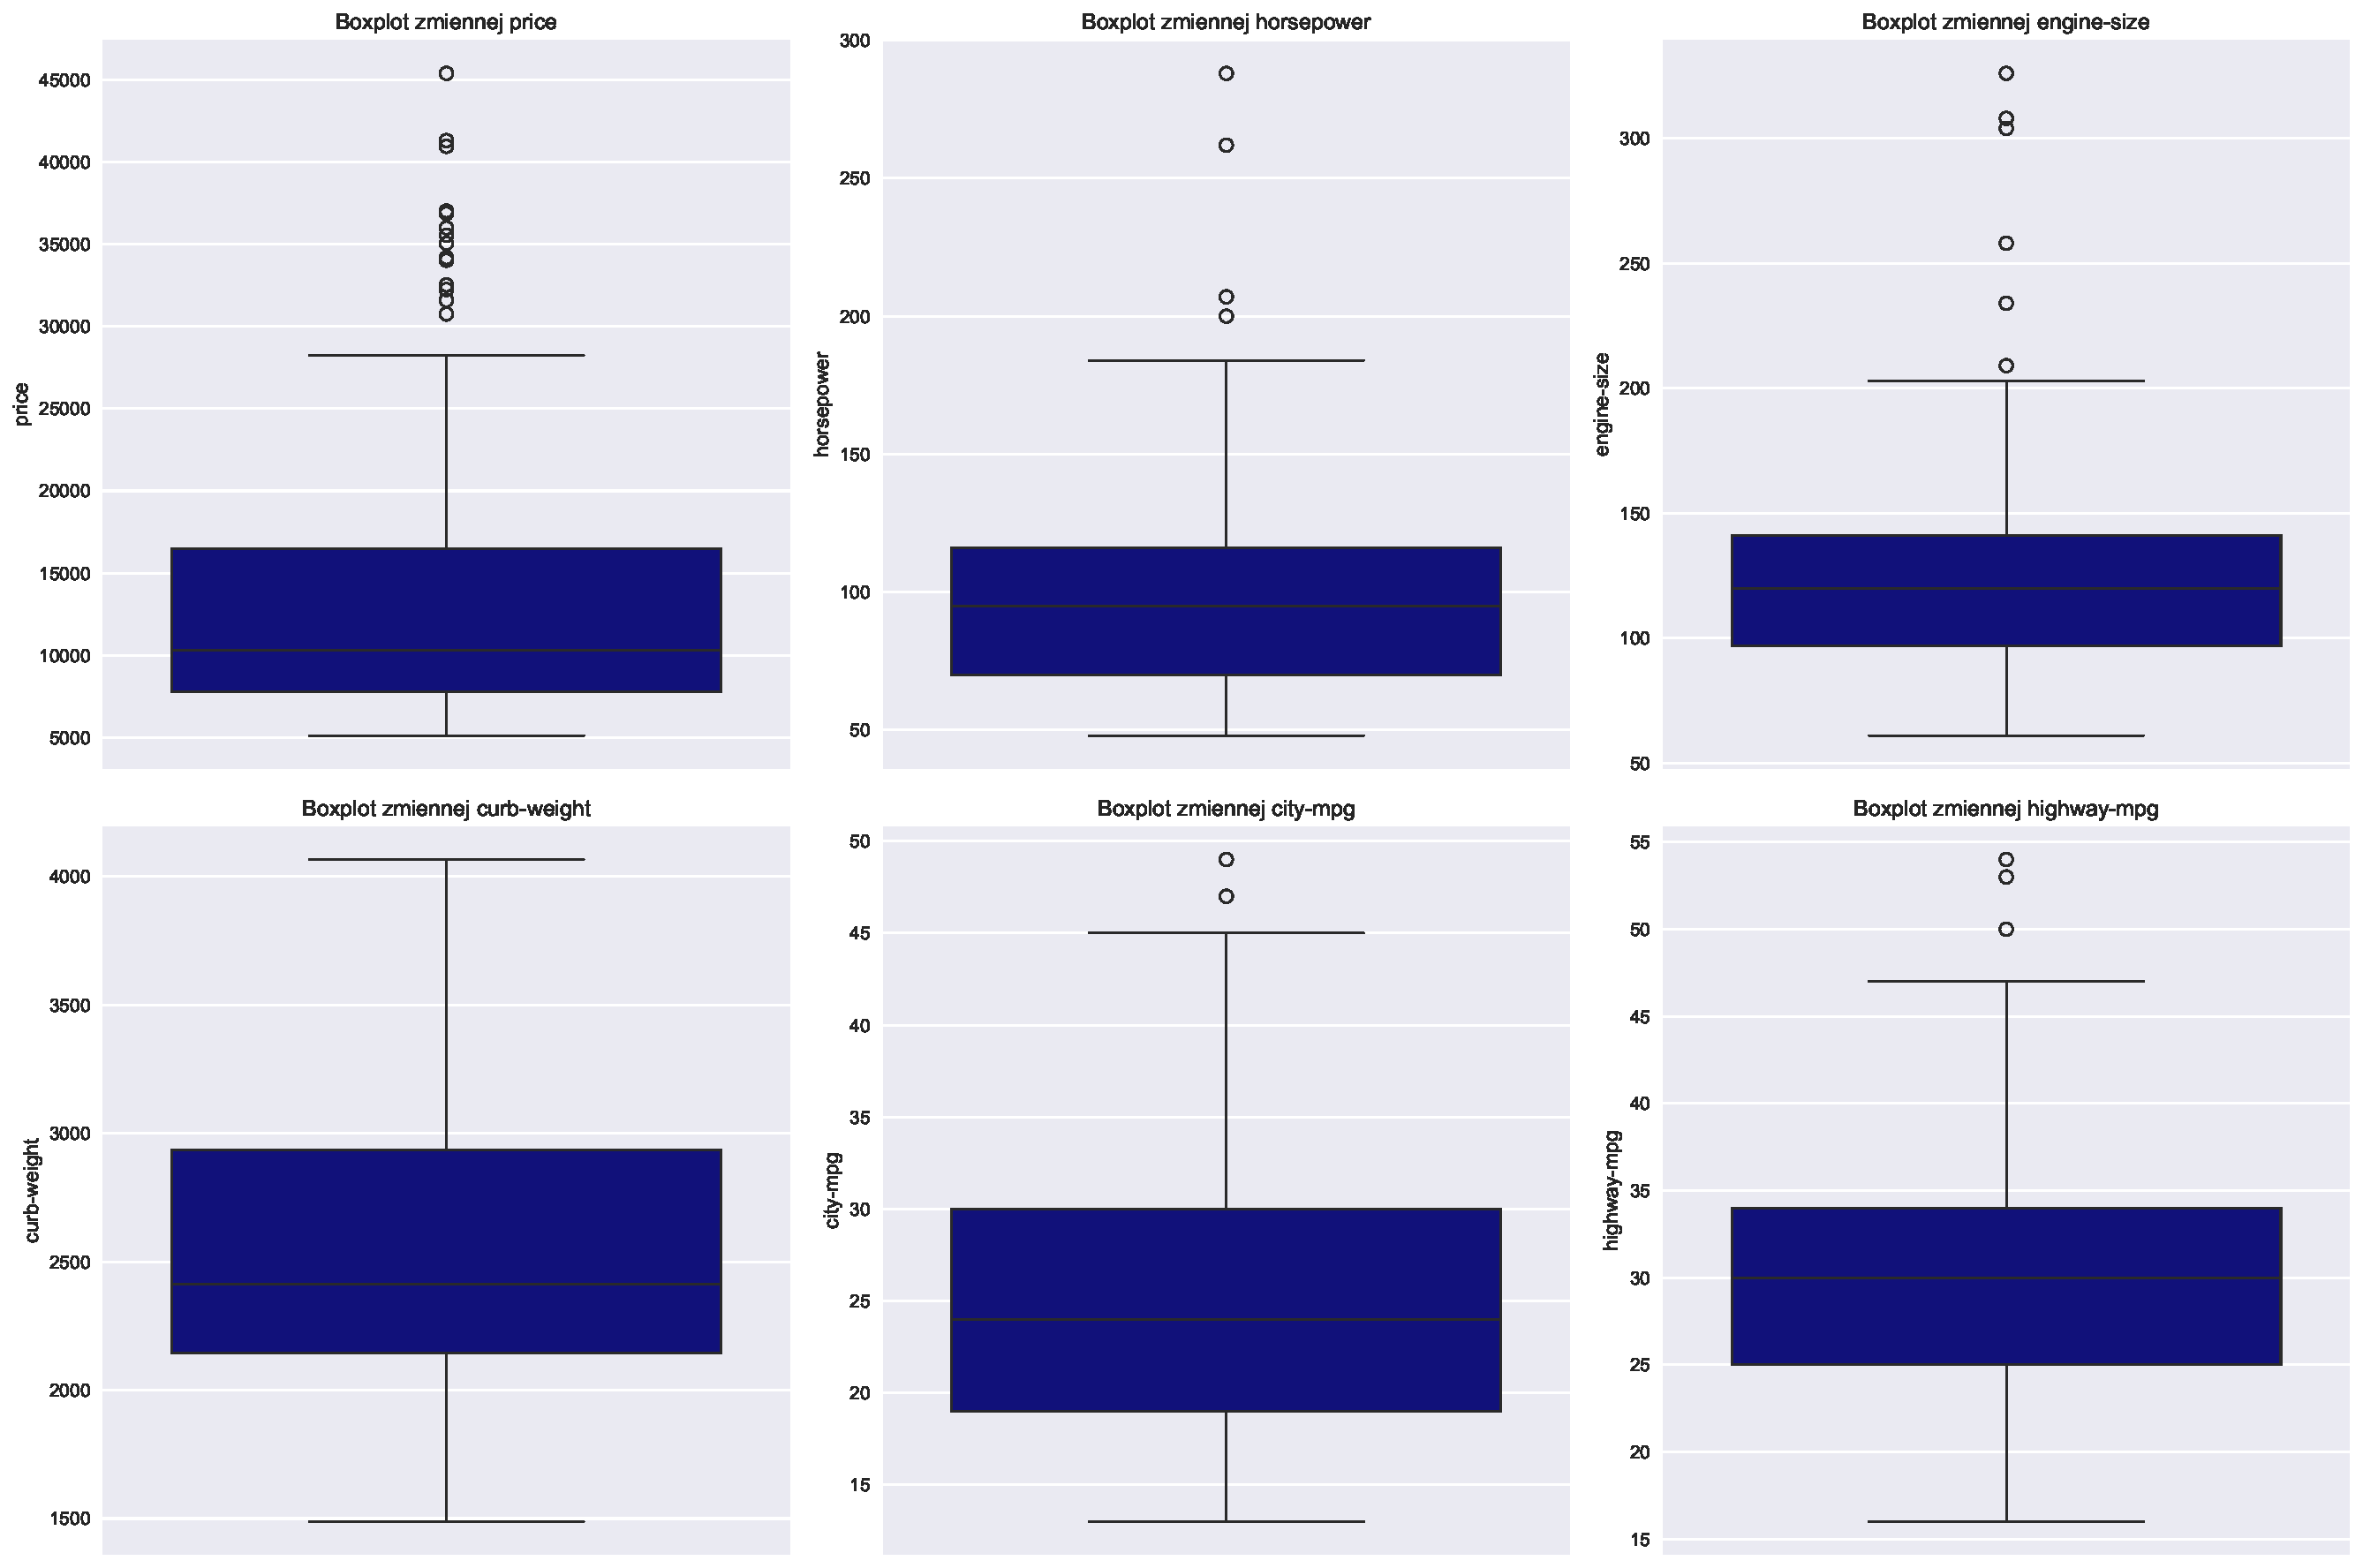
\includegraphics[width=0.9\textwidth]{boxplots.pdf}
    \caption{Boxploty dla wybranych zmiennych ciągłych}
    \label{fig:boxplots}
    \small\textit{Wykresy pudełkowe obrazujące strukturę kwartylową danych i potencjalne wartości odstające. Szczególnie widoczne są odstające wartości w zmiennych \texttt{price} i \texttt{horsepower}, co potwierdza obserwacje dotyczące asymetrii tych rozkładów.}
\end{figure}

\subsection{Wykresy kwantyl-kwantyl}

Wykresy Q-Q porównujące empiryczne kwantyle z kwantylami rozkładu normalnego potwierdziły odchylenia od normalności, szczególnie widoczne dla zmiennych o silnej asymetrii.

\begin{figure}[H]
    \centering
    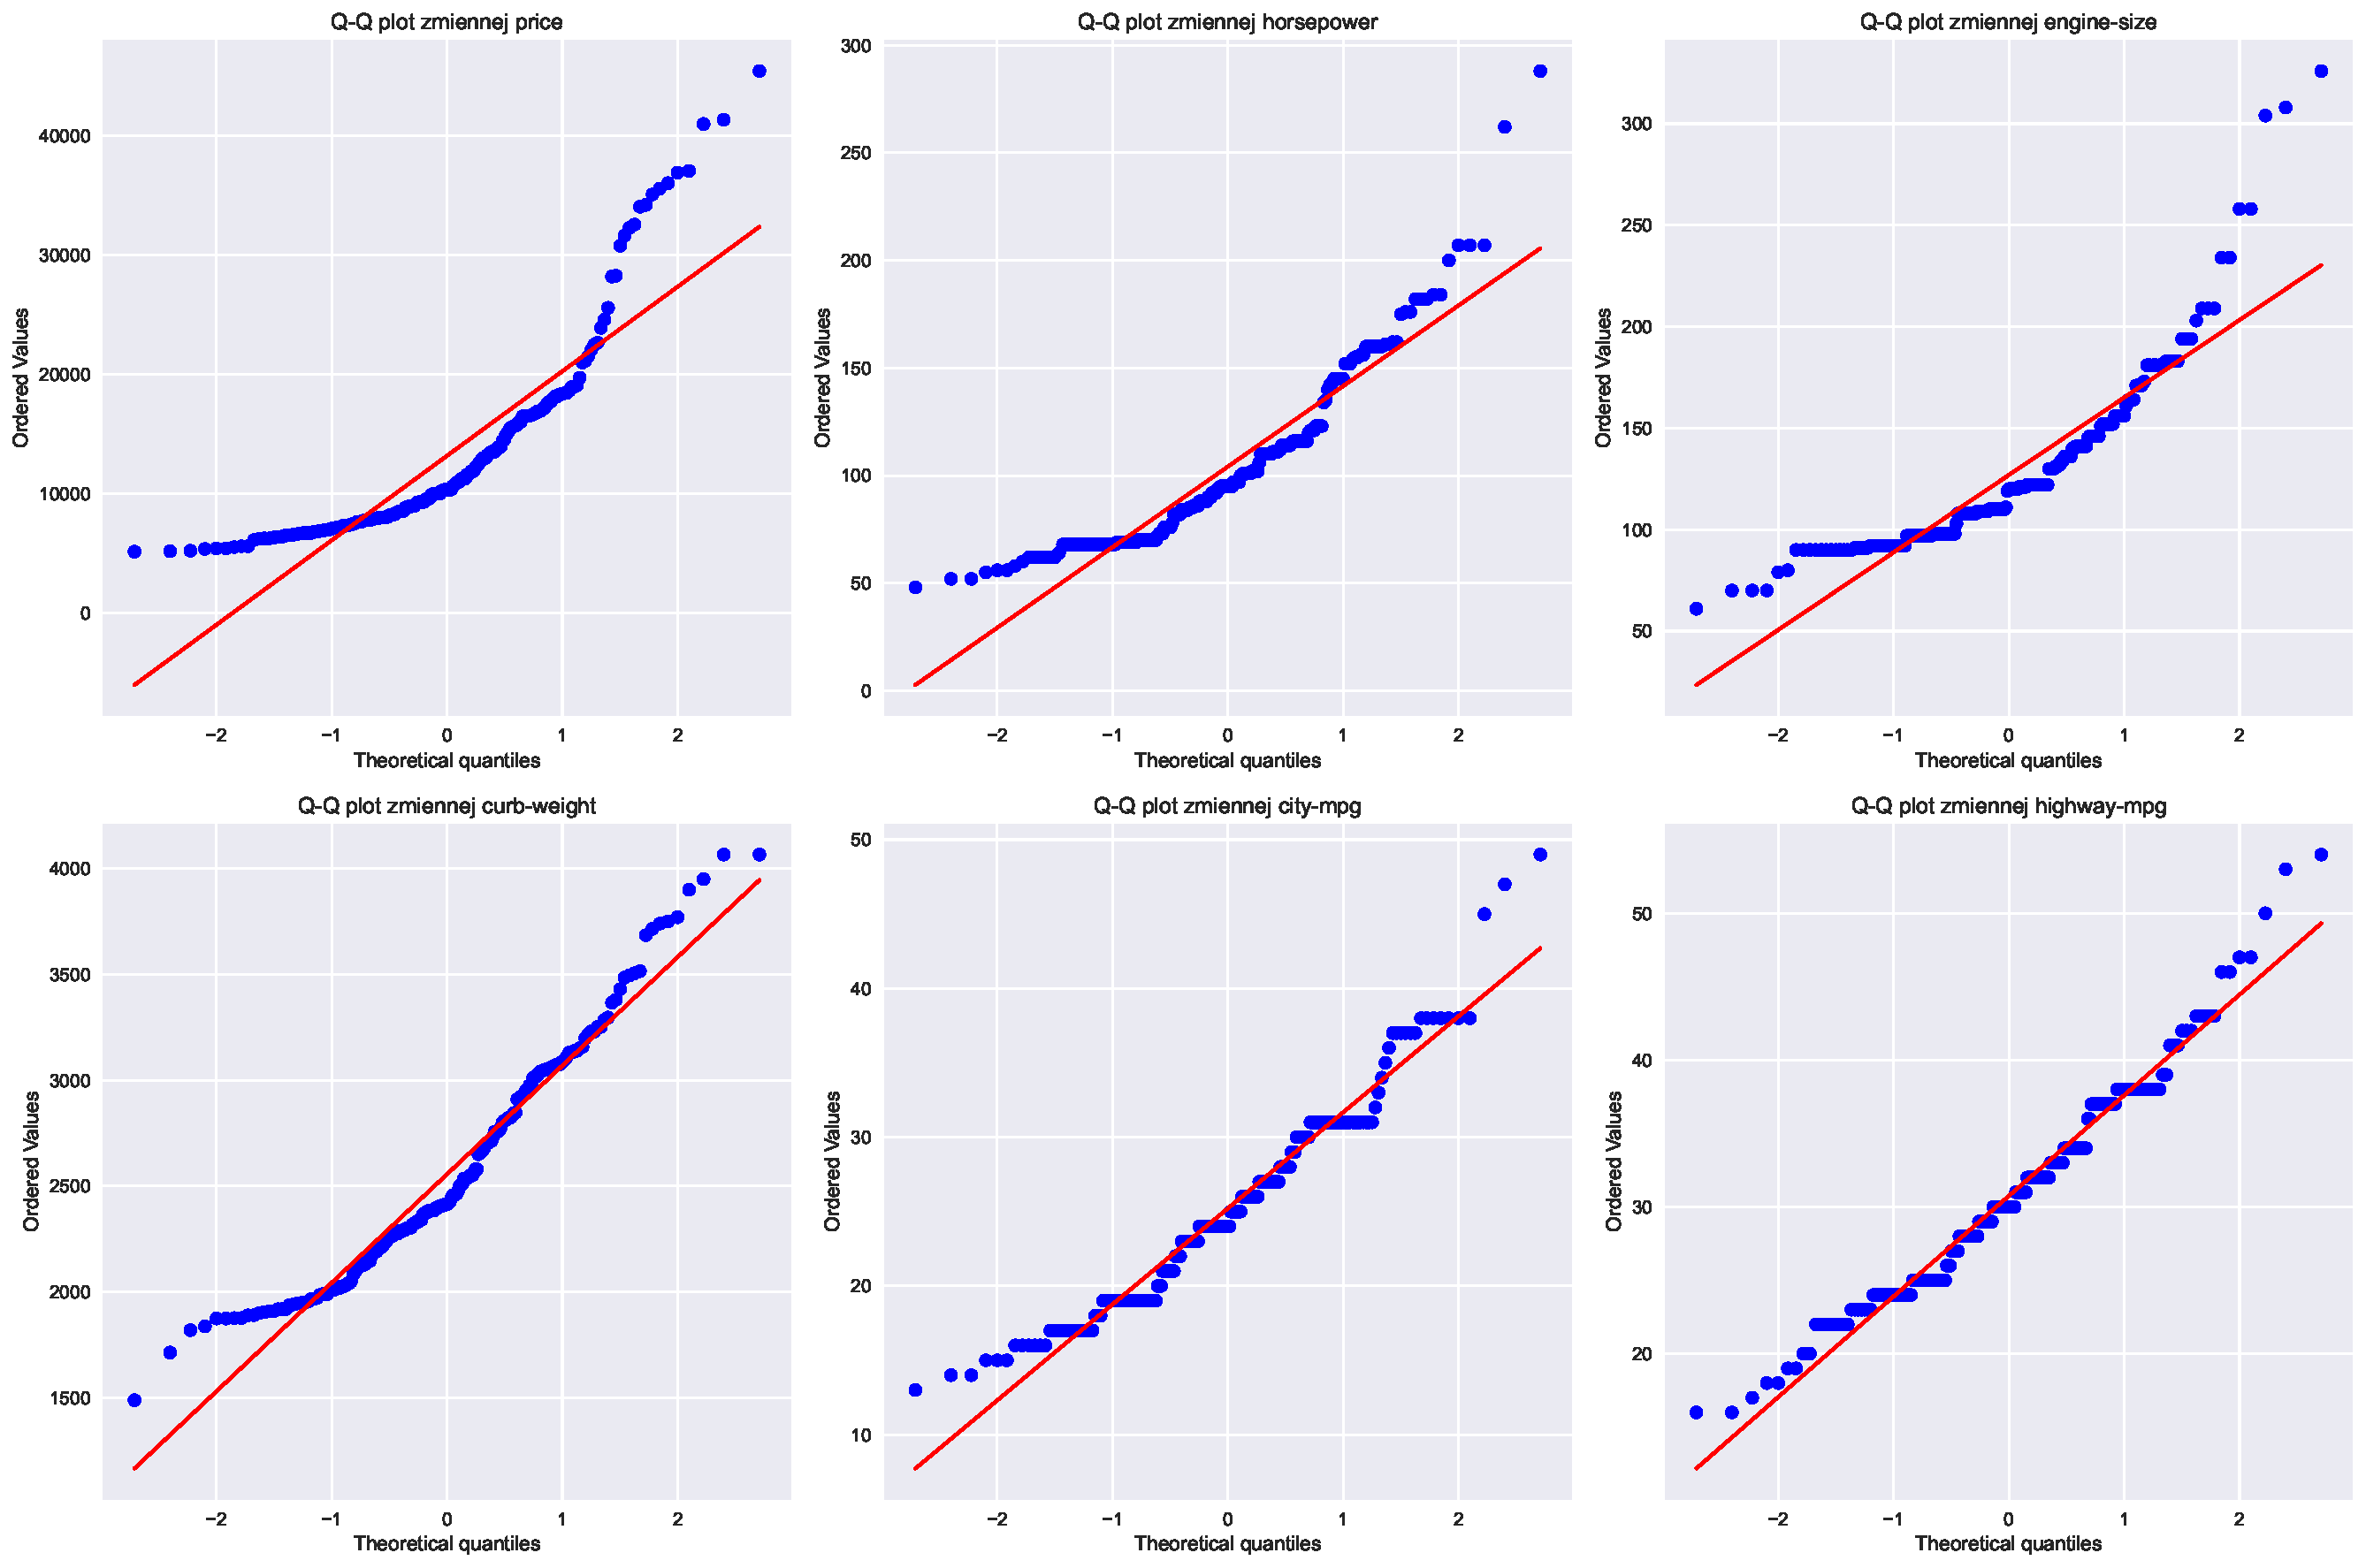
\includegraphics[width=0.9\textwidth]{qq_plots.pdf}
    \caption{Wykresy kwantyl-kwantyl (Q-Q) dla wybranych zmiennych}
    \label{fig:qq_plots}
    \small\textit{Wykresy Q-Q służące do oceny zgodności rozkładu empirycznego z rozkładem normalnym. Punkty leżące na linii oznaczają zgodność z rozkładem normalnym. Widoczne jest znaczne odchylenie od tej linii, szczególnie dla zmiennych \texttt{price} i \texttt{horsepower}, co potwierdza ich niezgodność z rozkładem normalnym.}
\end{figure}

\subsection{Wykresy gęstości (KDE)}

Krzywe gęstości jądrowej umożliwiły wizualizację kształtu rozkładów bez sztucznie narzucanych przedziałów histogramu. Szczególnie interesujący jest rozkład zmiennej \texttt{compression-ratio}, który wykazuje cechy rozkładu dwumodalnego, sugerując obecność dwóch różnych grup silników.

\begin{figure}[H]
    \centering
    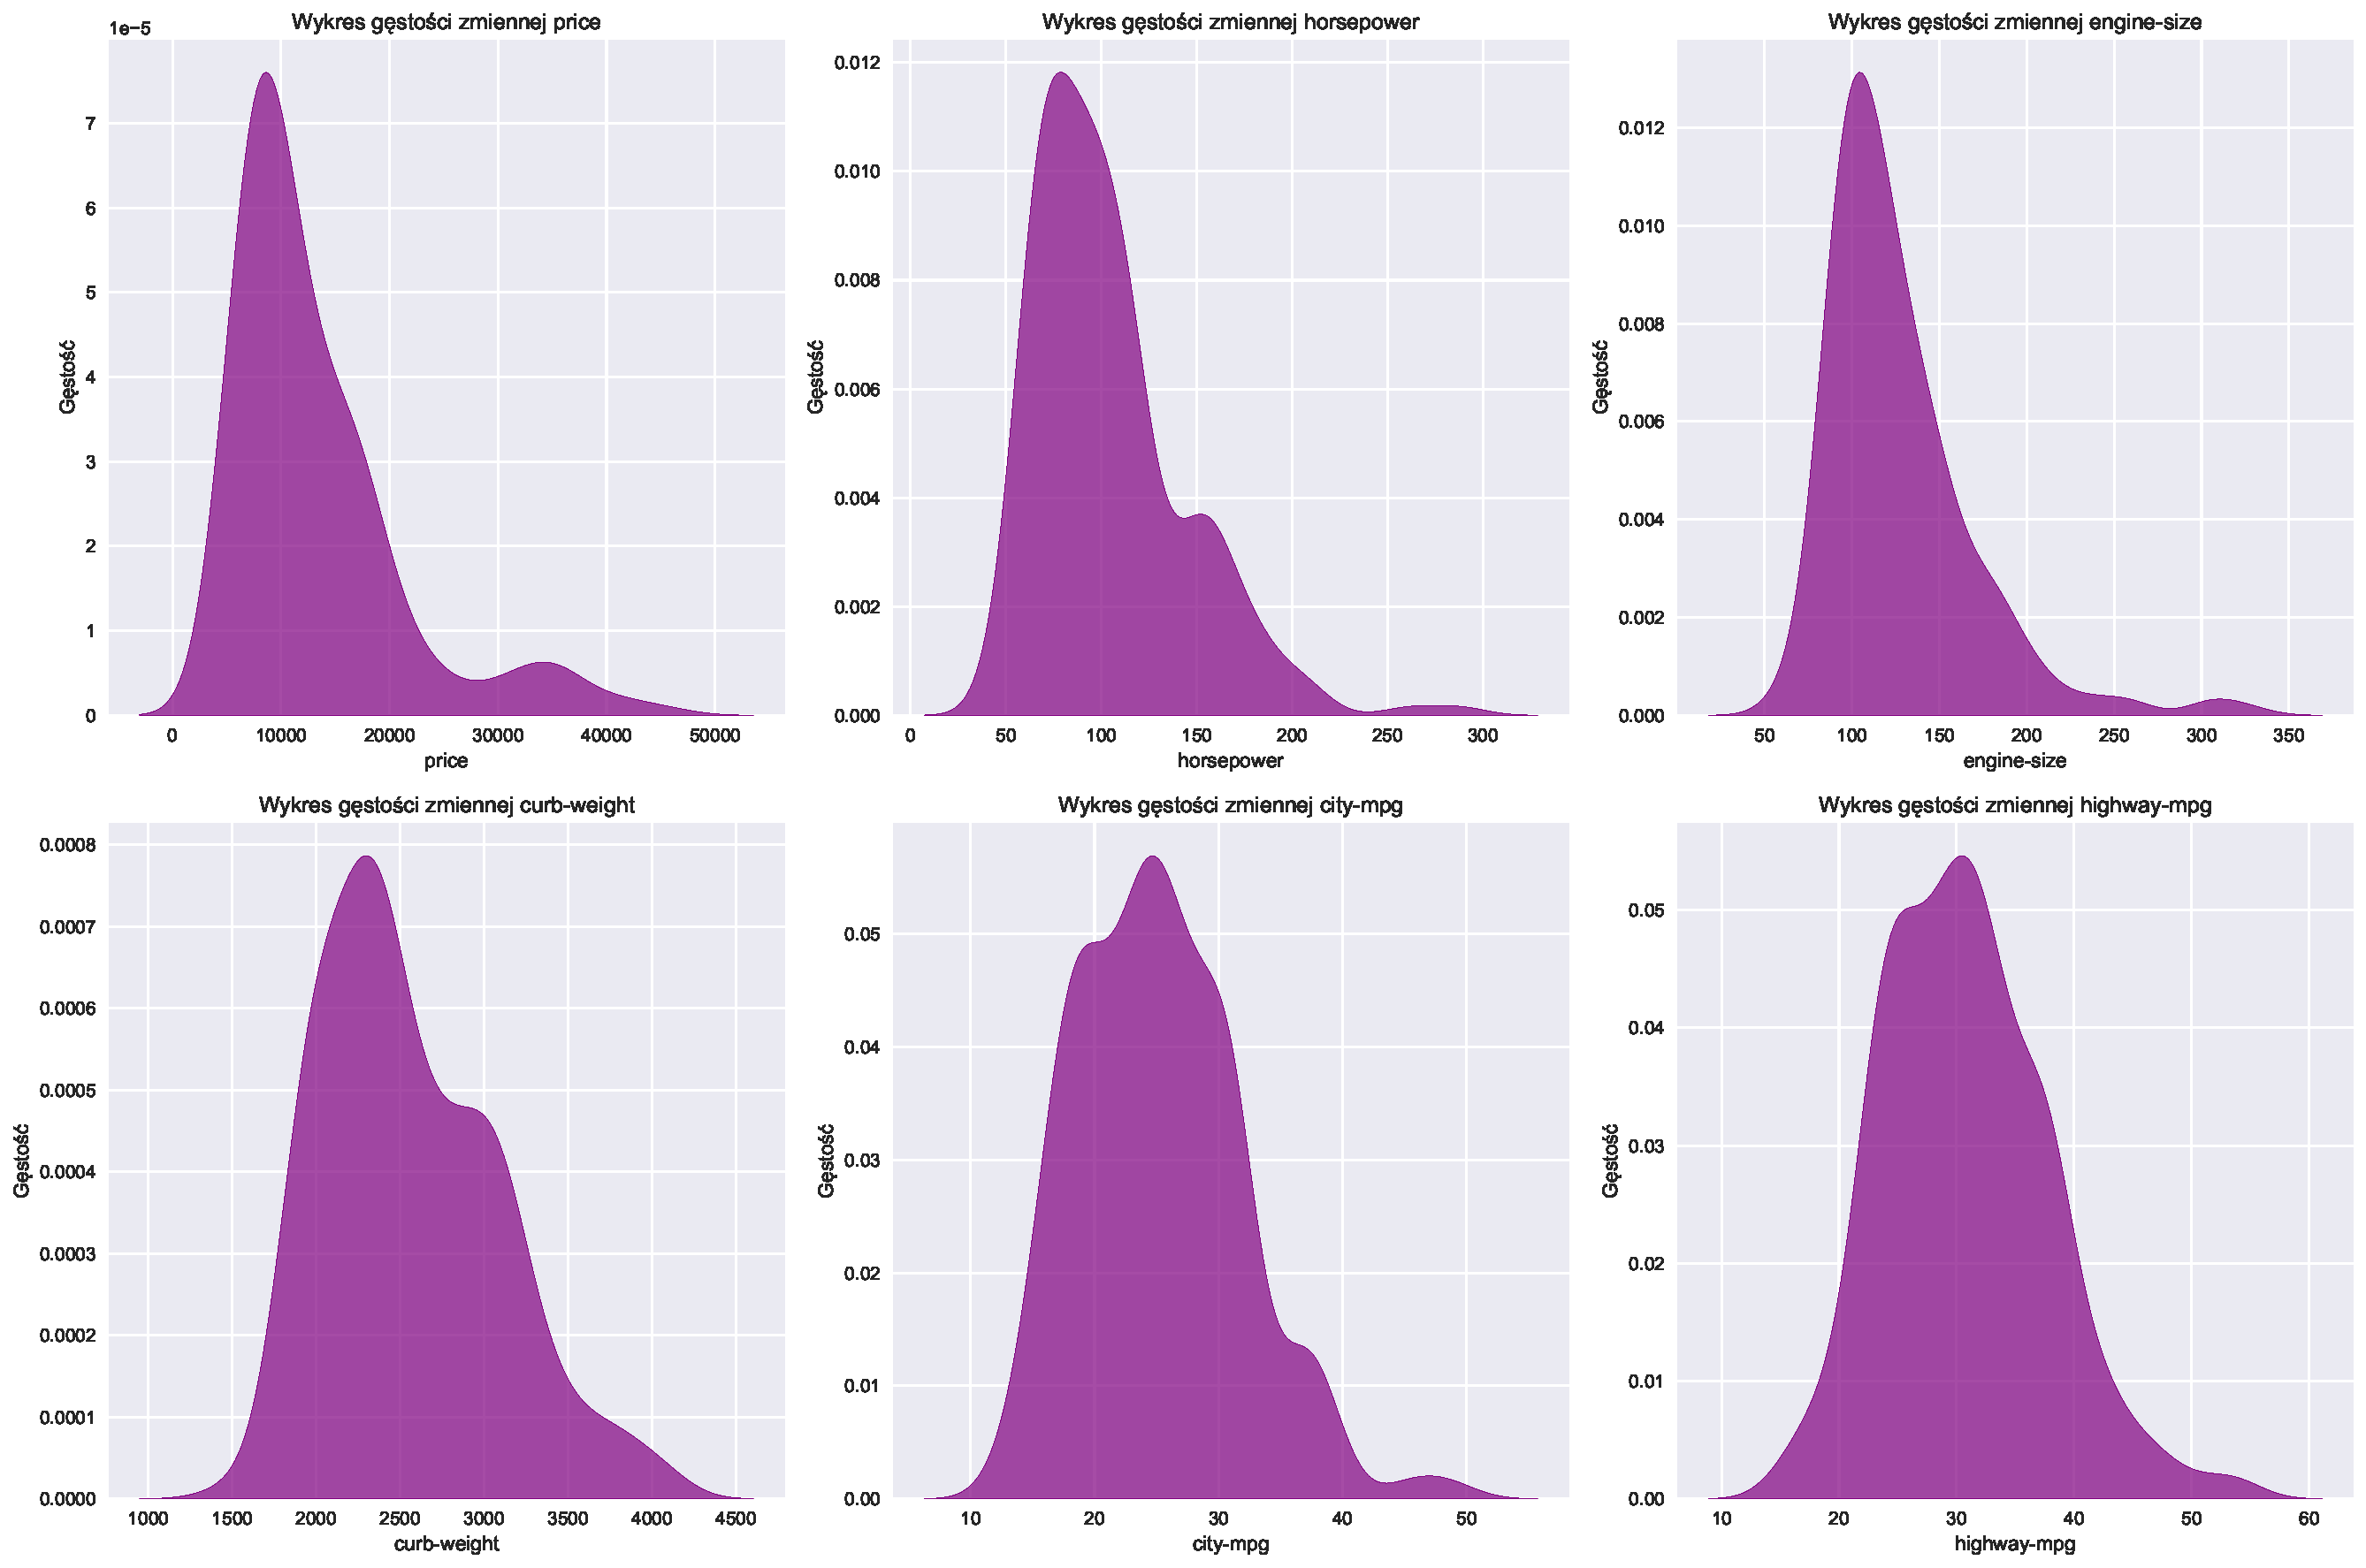
\includegraphics[width=0.9\textwidth]{kde_plots.pdf}
    \caption{Wykresy gęstości (KDE) dla wybranych zmiennych}
    \label{fig:kde_plots}
    \small\textit{Estymatory jądrowe gęstości dla kluczowych zmiennych, pozwalające na wygładzoną wizualizację rozkładów bez ograniczeń związanych z doborem liczby przedziałów histogramu.}
\end{figure}

\begin{figure}[H]
    \centering
    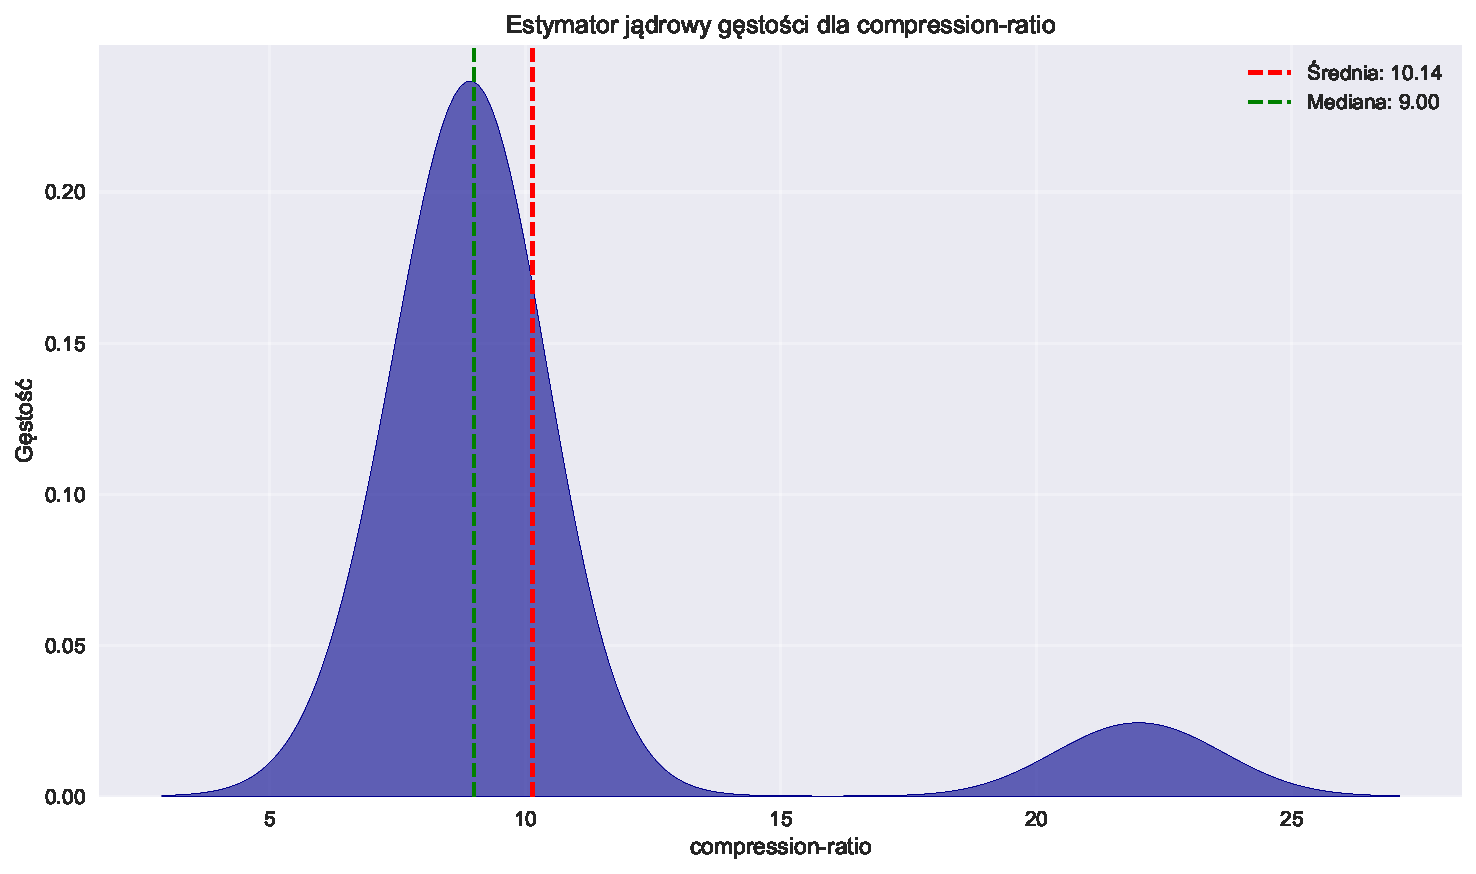
\includegraphics[width=0.75\textwidth]{kde_compression-ratio.pdf}
    \caption{Estymator jądrowy gęstości dla zmiennej compression-ratio}
    \label{fig:kde_compression_detail}
    \small\textit{Wykres gęstości dla zmiennej \texttt{compression-ratio}, ukazujący charakterystyczny dwumodalny rozkład. Dwa wyraźne szczyty sugerują obecność dwóch różnych grup silników, prawdopodobnie rozróżniających silniki benzynowe i wysokoprężne.}
\end{figure}

\subsection{Wykresy skrzypcowe}

Wykresy skrzypcowe połączyły zalety wykresów pudełkowych z wizualizacją gęstości, dając pełniejszy obraz rozkładów analizowanych zmiennych.

\kod{
# 1. STANDARDOWE WYKRESY SKRZYPCOWE
fig_violin, axes = plt.subplots(2, 3, figsize=(18, 12))
axes = axes.flatten()

for i, var in enumerate(selected_variables):
    sns.violinplot(y=df[var], ax=axes[i], color='purple')
    axes[i].set_title(f'Wykres skrzypcowy zmiennej {var}')
    axes[i].set_ylabel(var)

plt.tight_layout()
# Save violin plots
save_fig(fig_violin, 'violin_plots', directory='figures')
plt.show()

# 2. WYKRESY SKRZYPCOWE WEDŁUG KATEGORII
fig_violin_cat, axes = plt.subplots(2, 3, figsize=(18, 12))
axes = axes.flatten()

for i, var in enumerate(selected_variables):
    sns.violinplot(x='num-of-cylinders', y=var, data=df, ax=axes[i], palette='viridis')
    axes[i].set_title(f'Rozkład {var} w zależności od liczby cylindrów')
    axes[i].set_xlabel('Liczba cylindrów')
    axes[i].set_ylabel(var)

plt.tight_layout()
# Save violin plots by category
save_fig(fig_violin_cat, 'violin_plots_by_cylinder', directory='figures')
plt.show()

# 3. STRIP PLOTS (DOT PLOTS) WEDŁUG KATEGORII
fig_strip, axes = plt.subplots(2, 3, figsize=(18, 12))
axes = axes.flatten()

for i, var in enumerate(selected_variables):
    sns.stripplot(x='num-of-cylinders', y=var, data=df, ax=axes[i], palette='Set2', 
                  size=5, jitter=True, alpha=0.7)
    axes[i].set_title(f'Rozkład punktowy {var} według liczby cylindrów')
    axes[i].set_xlabel('Liczba cylindrów')
    axes[i].set_ylabel(var)

plt.tight_layout()
# Save strip plots
save_fig(fig_strip, 'strip_plots_by_cylinder', directory='figures')
plt.show()
}{Kod tworzący wykresy skrzypcowe standardowe oraz z podziałem na kategorie, a także wykresy rozrzutu punktowego}

\begin{figure}[H]
    \centering
    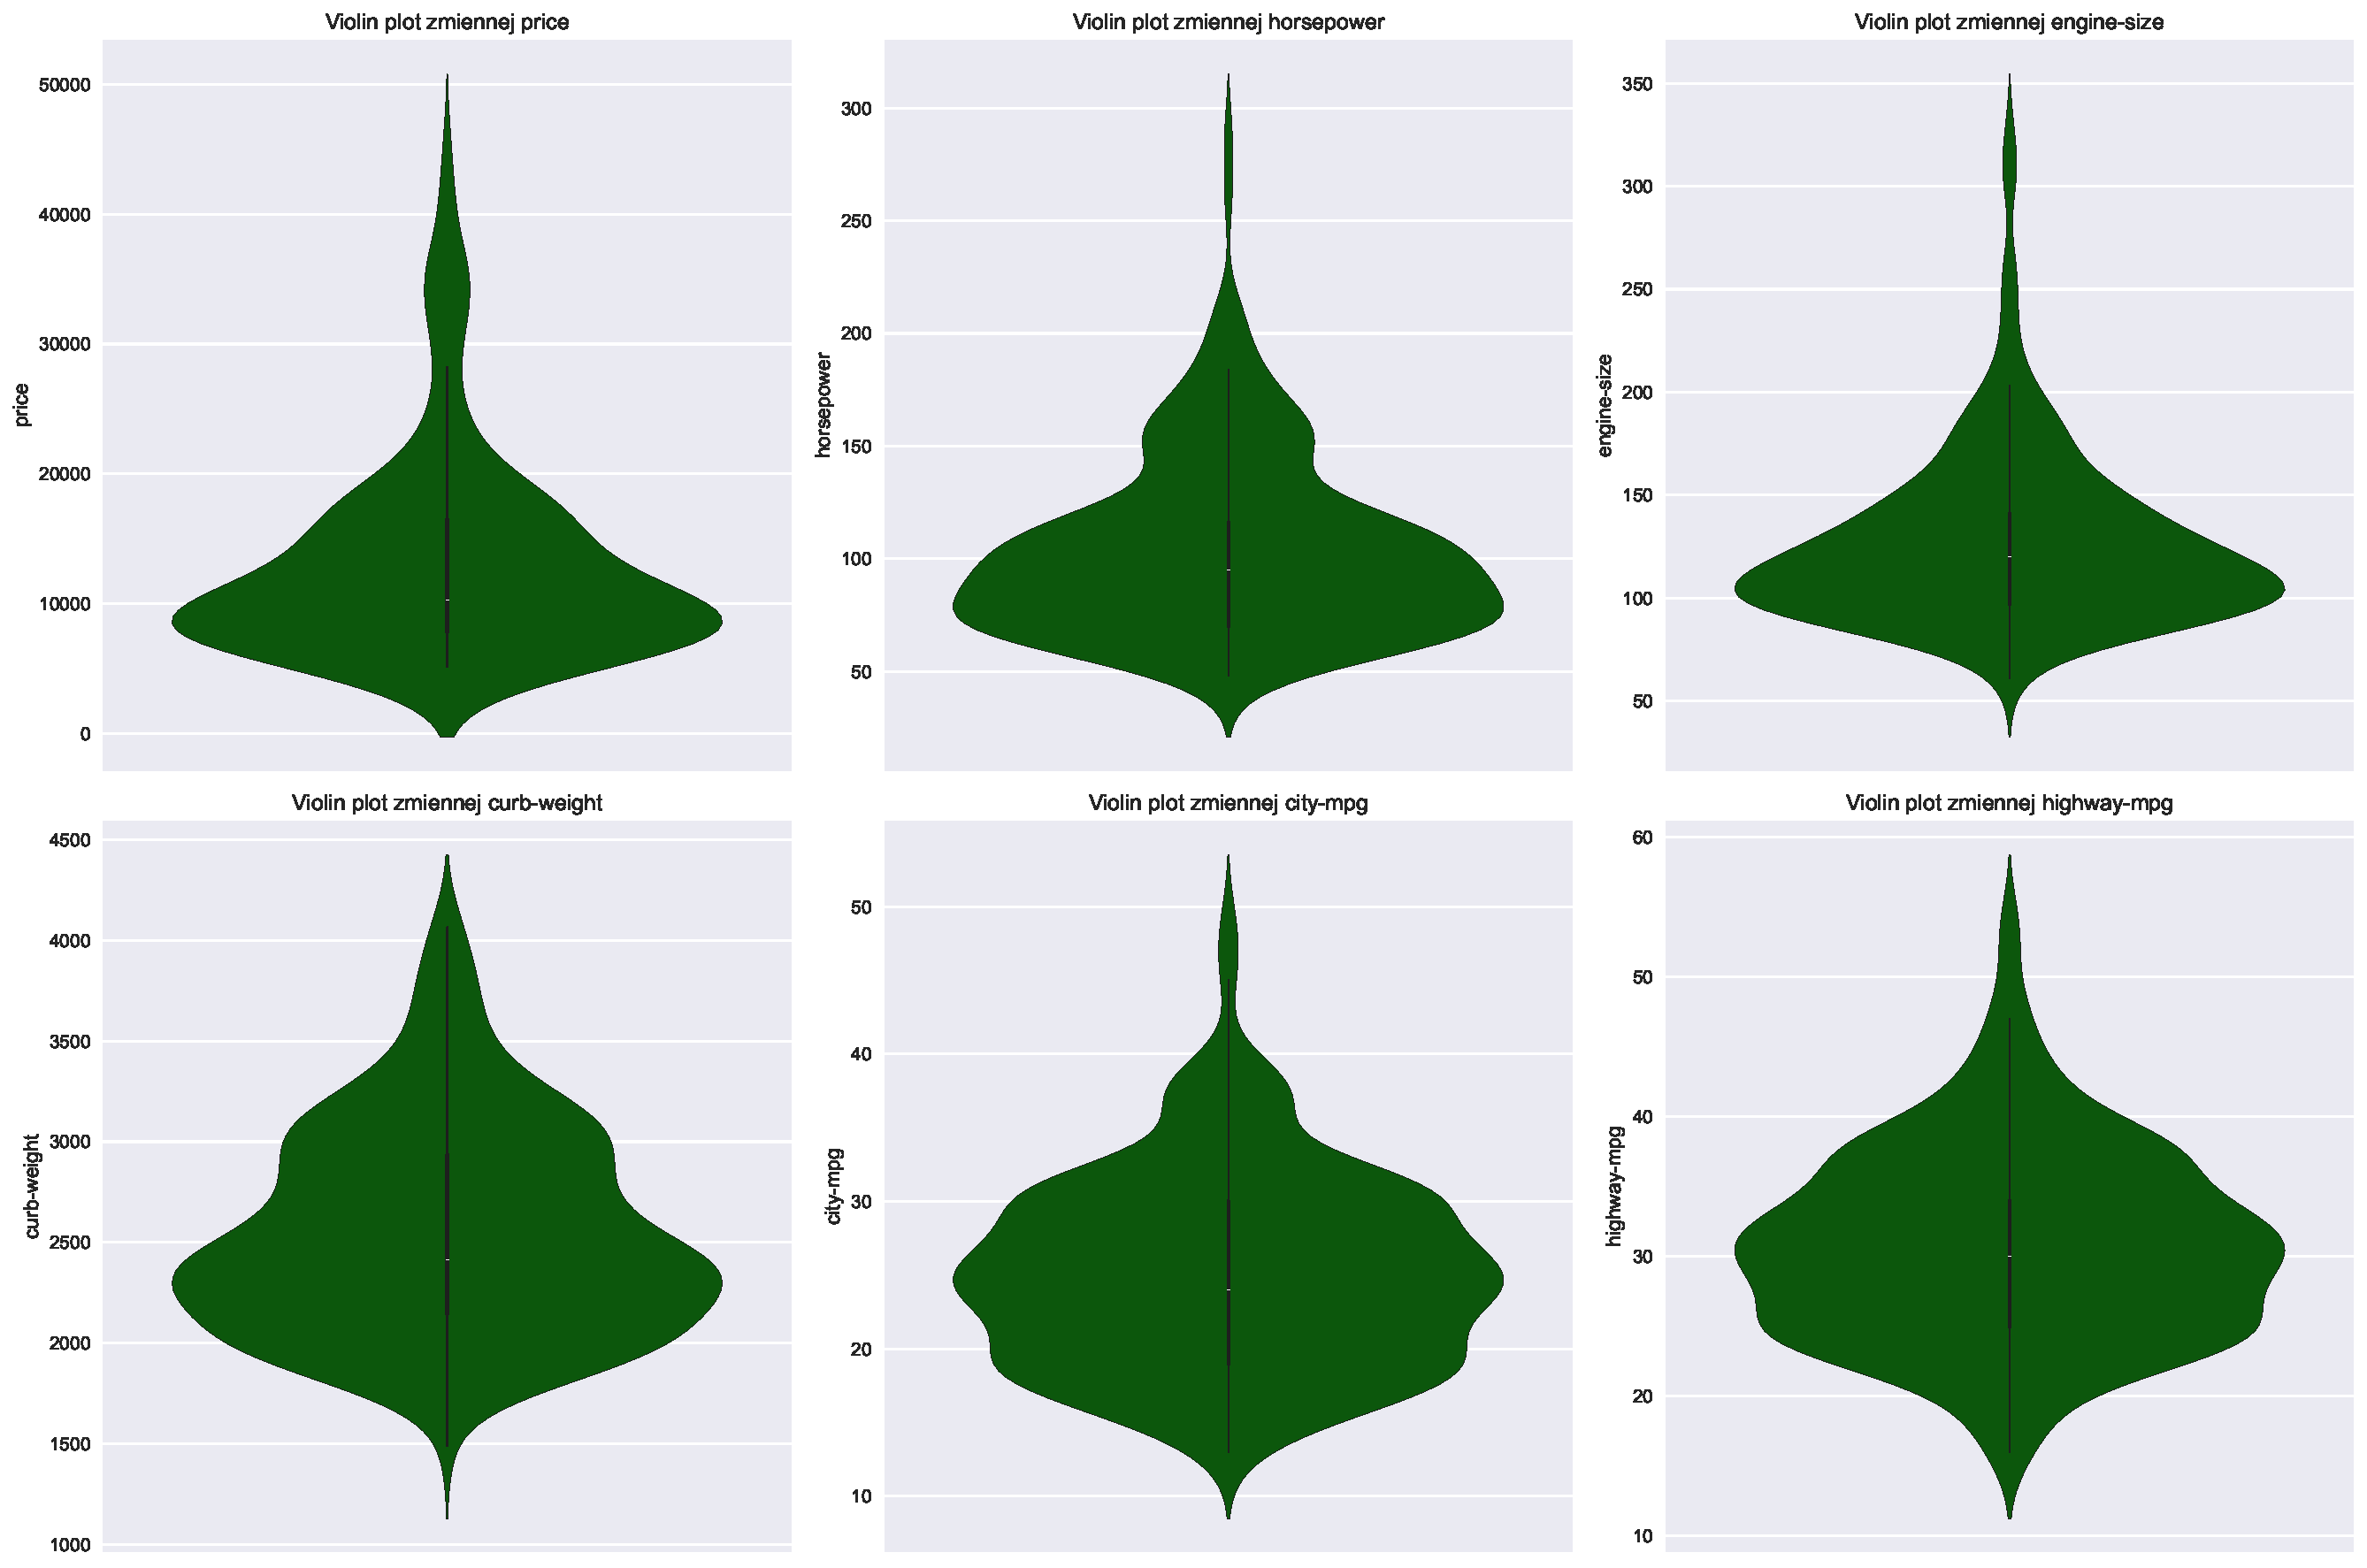
\includegraphics[width=0.9\textwidth]{violin_plots.pdf}
    \caption{Wykresy skrzypcowe dla wybranych zmiennych}
    \label{fig:violin_plots}
    \small\textit{Wykresy skrzypcowe łączące cechy wykresów pudełkowych z wizualizacją gęstości rozkładu. Kształt "skrzypiec" obrazuje jak zmienia się gęstość zmiennej w różnych przedziałach jej wartości.}
\end{figure}

\begin{figure}[H]
    \centering
    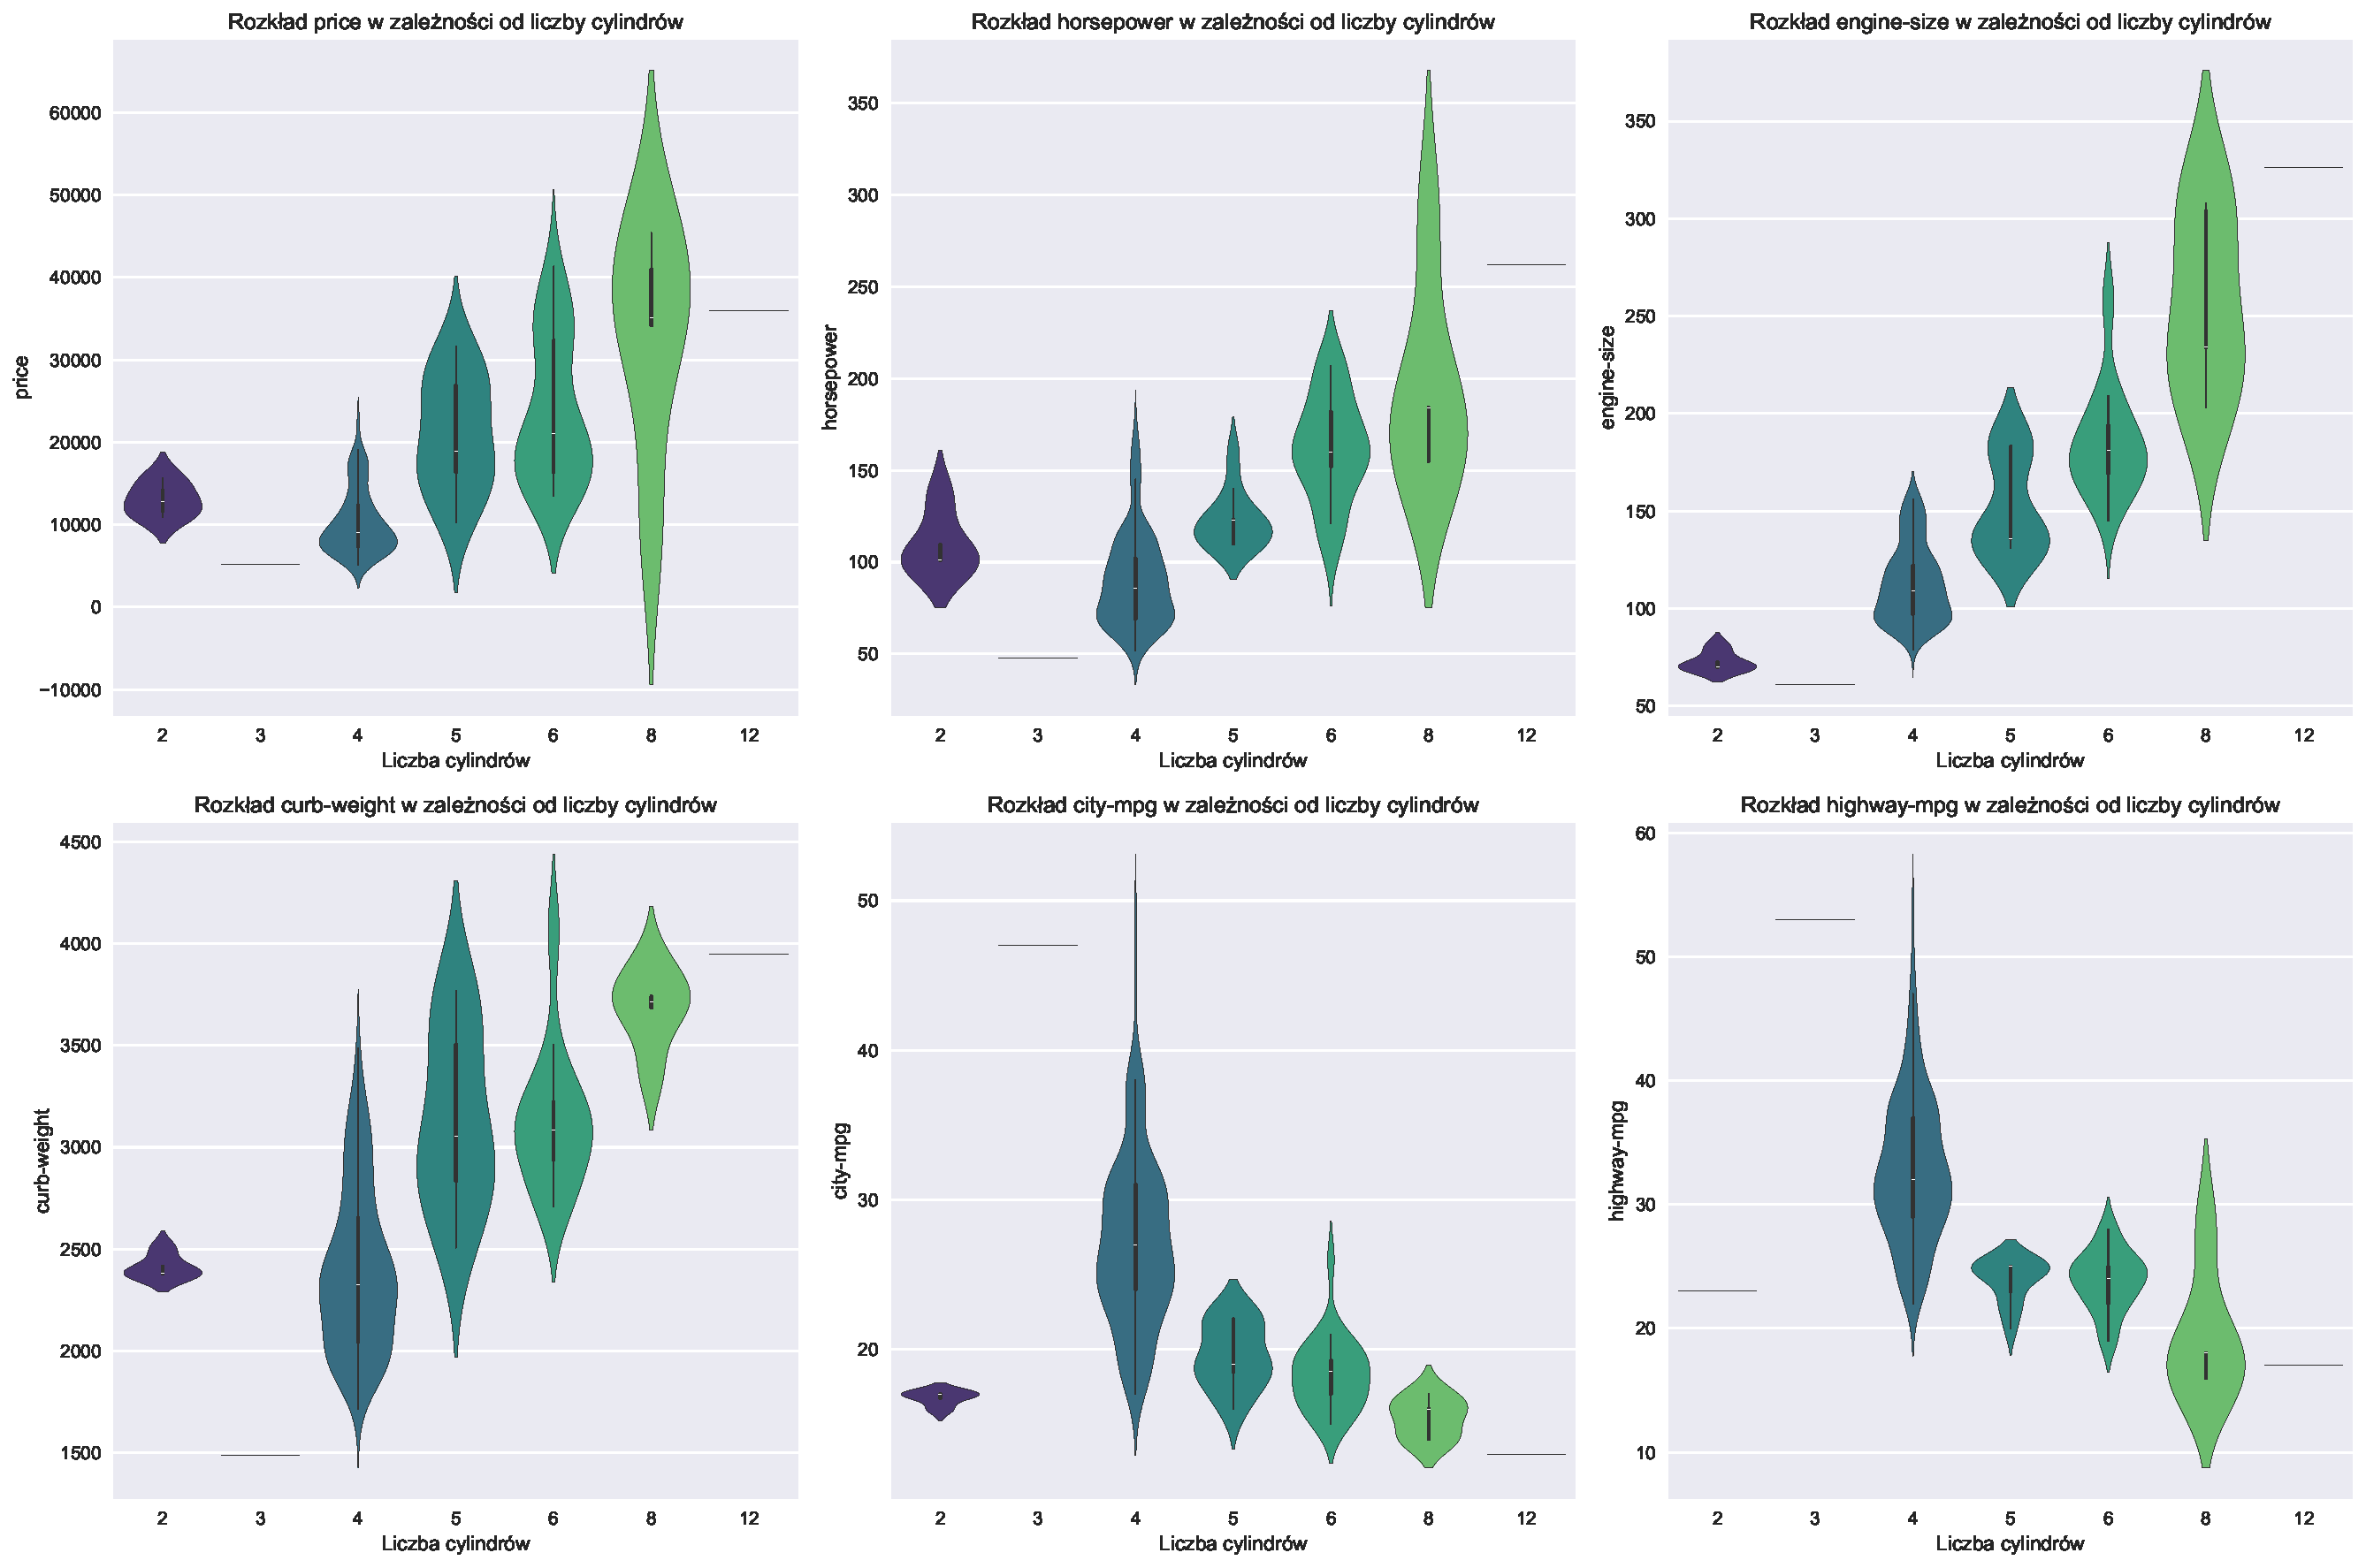
\includegraphics[width=0.9\textwidth]{violin_plots_by_cylinder.pdf}
    \caption{Wykresy skrzypcowe w zależności od liczby cylindrów}
    \label{fig:violin_plots_cylinder}
    \small\textit{Wykresy skrzypcowe przedstawiające rozkład zmiennych numerycznych w zależności od liczby cylindrów silnika. Widoczny jest wyraźny wzrost ceny, mocy i pojemności silnika wraz ze wzrostem liczby cylindrów.}
\end{figure}

\subsection{Dystrybuanty empiryczne}

Wykresy dystrybuant empirycznych pozwoliły na ocenę prawdopodobieństwa nieprzekroczenia określonych wartości dla poszczególnych zmiennych.

\kod{
# 1. DYSTRYBUANTY EMPIRYCZNE (CDF)
fig_cdf, axes = plt.subplots(2, 3, figsize=(18, 12))
axes = axes.flatten()

for i, var in enumerate(selected_variables):
    # Sortowanie danych
    x = np.sort(df[var])
    # Obliczanie wartości CDF (dystrybuanty empirycznej)
    y = np.arange(1, len(x) + 1) / len(x)
    
    axes[i].plot(x, y, marker='.', linestyle='none', alpha=0.5, color='navy')
    axes[i].plot(x, y, color='red', alpha=0.7)
    
    axes[i].set_title(f'Dystrybuanta empiryczna zmiennej {var}')
    axes[i].set_xlabel(var)
    axes[i].set_ylabel('Prawdopodobieństwo')
    axes[i].grid(True, alpha=0.3)

plt.tight_layout()
# Save CDF plots
save_fig(fig_cdf, 'cdf_plots', directory='figures')
plt.show()

# 2. MACIERZ WYKRESÓW PAR (PAIRPLOT)
fig_pairplot = sns.pairplot(df[selected_variables], diag_kind='kde', height=2.5)
plt.suptitle('Wykresy par dla wybranych zmiennych', y=1.02)
# Save pairplot matrix
save_fig(fig_pairplot, 'pairplot_matrix', directory='figures')
plt.show()
}{Kod tworzący wykresy dystrybuant empirycznych oraz macierz wykresów par}

\begin{figure}[H]
    \centering
    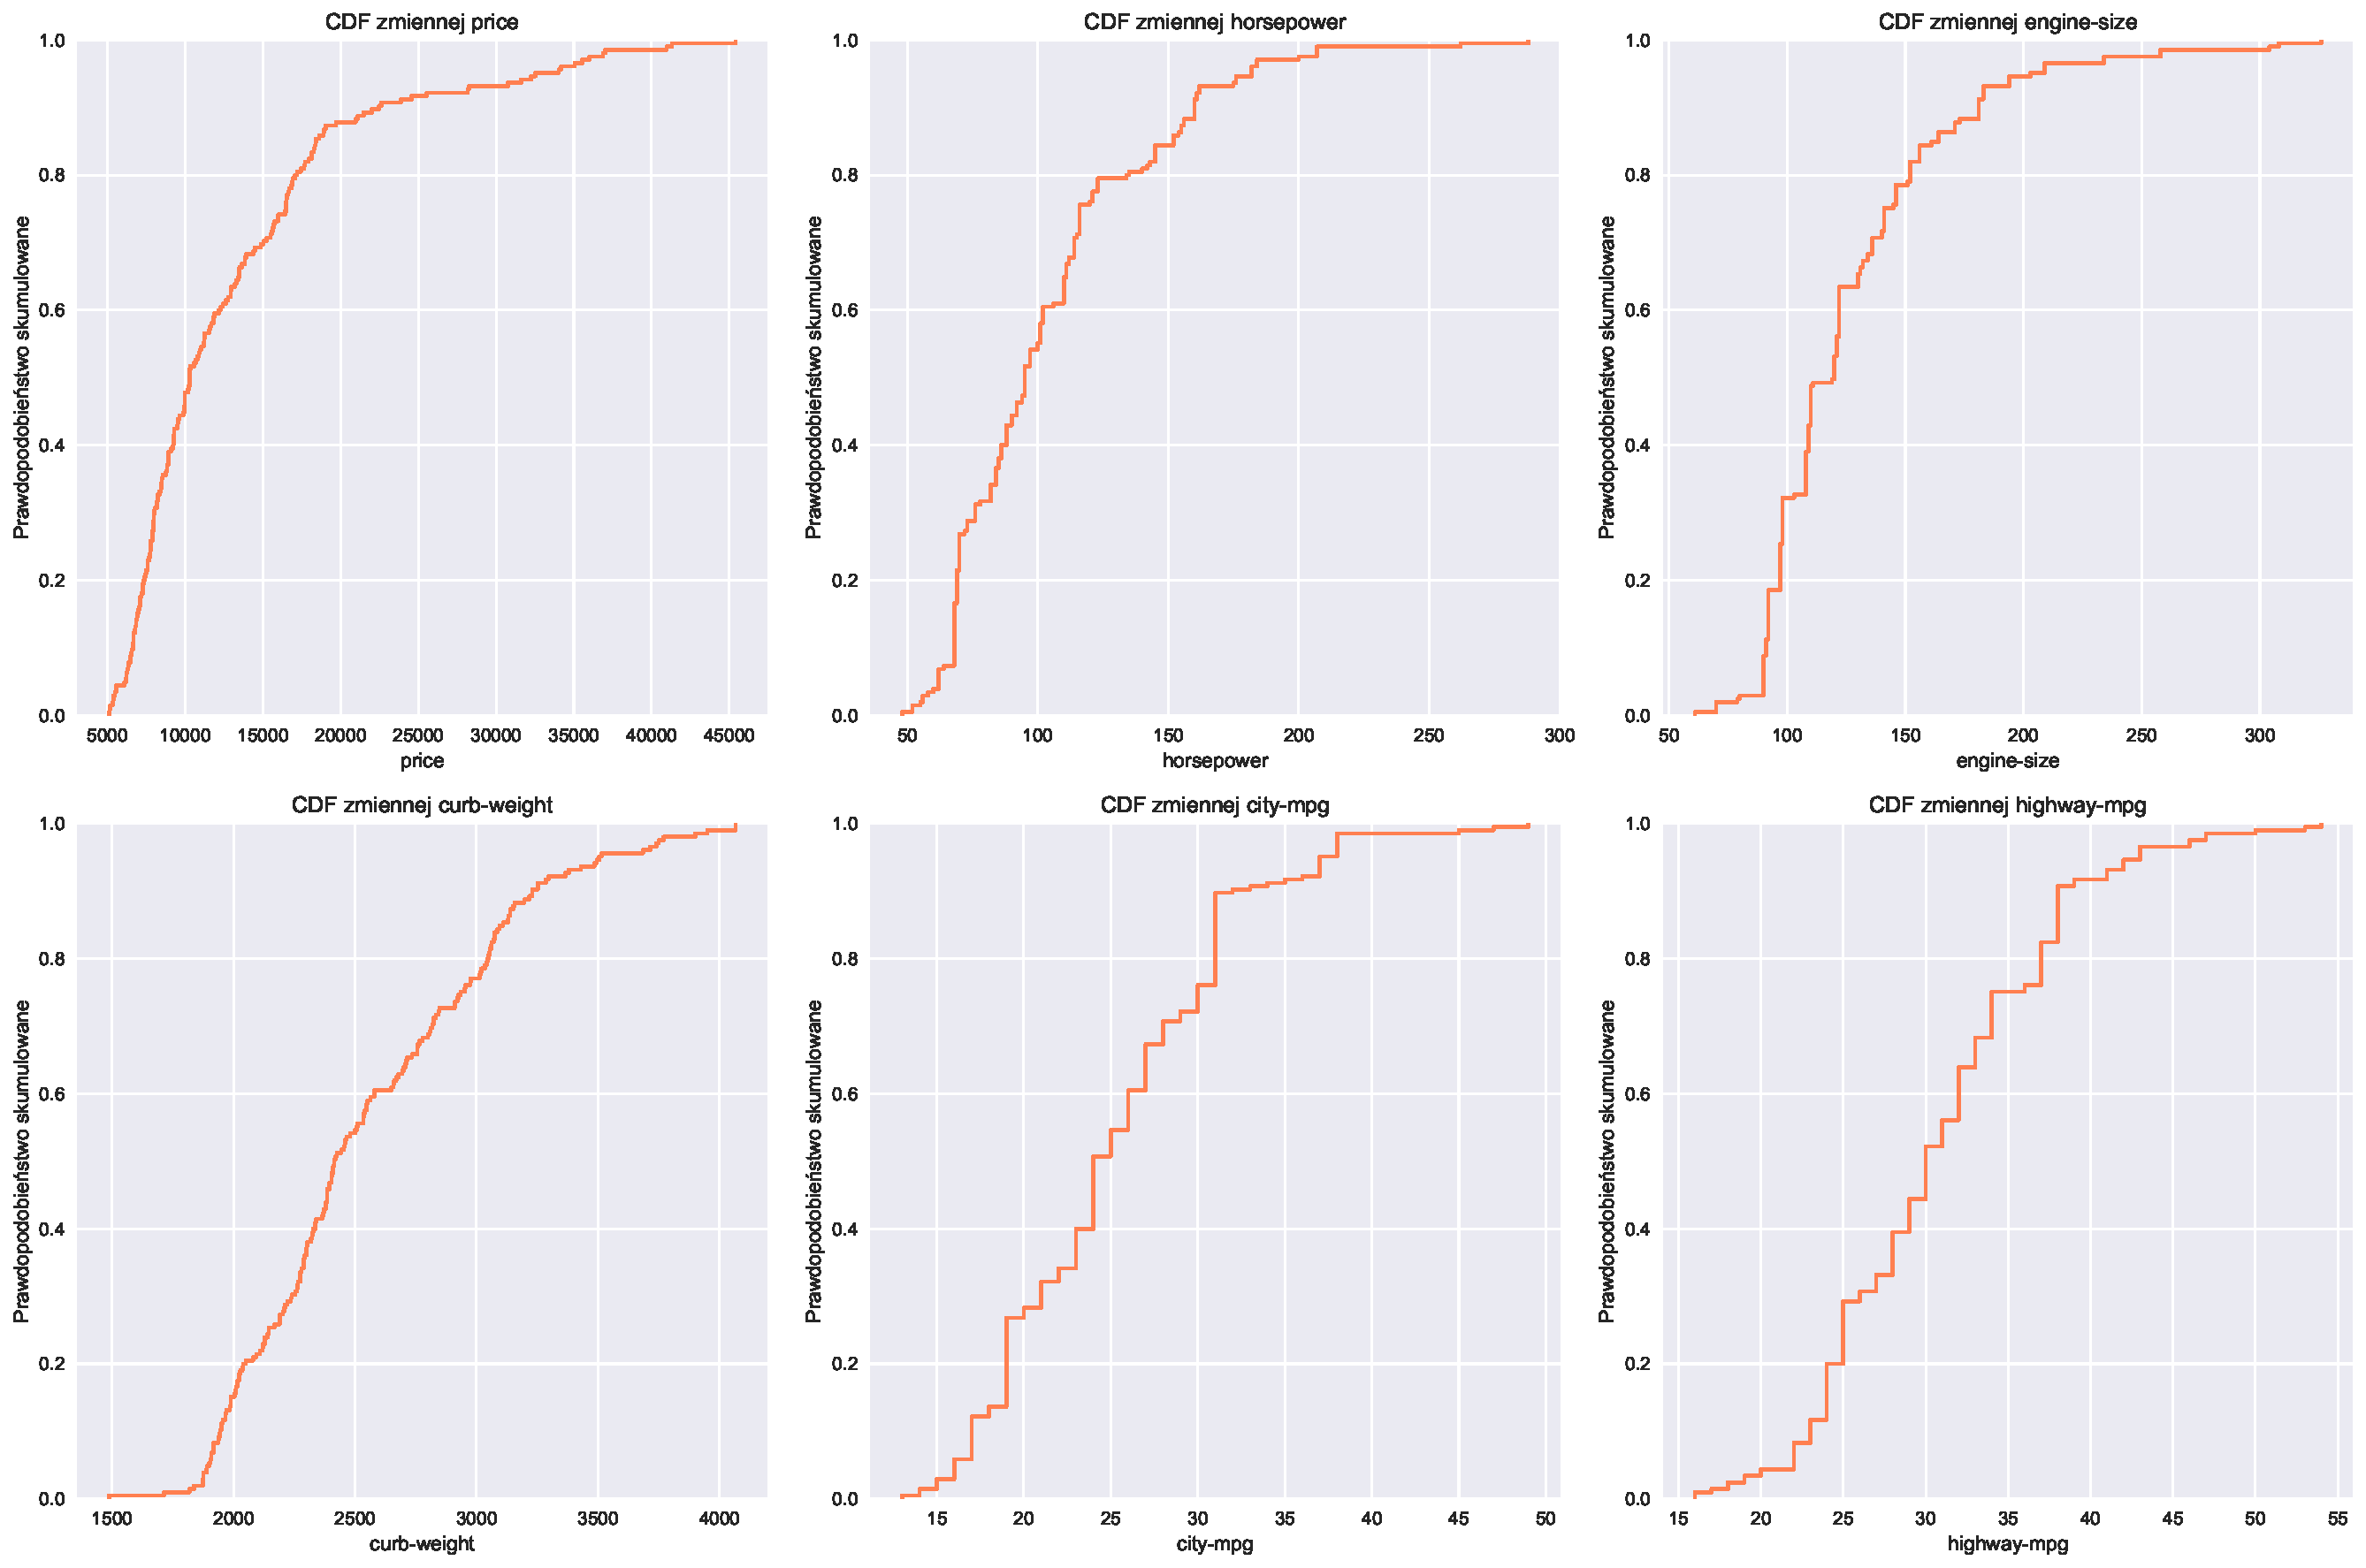
\includegraphics[width=0.9\textwidth]{cdf_plots.pdf}
    \caption{Dystrybuanty empiryczne dla wybranych zmiennych}
    \label{fig:cdf_plots}
    \small\textit{Dystrybuanty empiryczne (CDF) dla analizowanych zmiennych. Wykresy te pozwalają na określenie prawdopodobieństwa, że zmienna nie przekroczy danej wartości.}
\end{figure}

\subsection{Macierz korelacji}

\kod{
# CORRELATION HEATMAP
fig_corr = plt.figure(figsize=(14, 10))
corr_matrix = df[numeric_cols].corr()
mask = np.triu(np.ones_like(corr_matrix, dtype=bool))
sns.heatmap(corr_matrix, mask=mask, annot=True, cmap='coolwarm', fmt='.2f', linewidths=0.5)
plt.title('Macierz korelacji dla zmiennych numerycznych')
# Save correlation heatmap
save_fig(fig_corr, 'correlation_heatmap', directory='figures')
plt.show()

# Save correlation matrix to CSV for LaTeX report
corr_matrix.round(2).to_csv('figures/correlation_matrix.csv')

# SCATTER PLOT WITH CATEGORICAL VARIABLE
fig_scatter_cat = plt.figure(figsize=(10, 8))
sns.scatterplot(data=df, x='horsepower', y='price', hue='body-style', palette='viridis')
plt.title('Zależność między mocą silnika a ceną samochodu')
plt.xlabel('Moc silnika (hp)')
plt.ylabel('Cena ($)')
plt.legend(title='Typ nadwozia')
save_fig(fig_scatter_cat, 'scatter_hp_price_by_body', directory='figures')
plt.show()
}{Kod generujący macierz korelacji i wykres rozproszenia z podziałem na kategorie}

\begin{figure}[H]
    \centering
    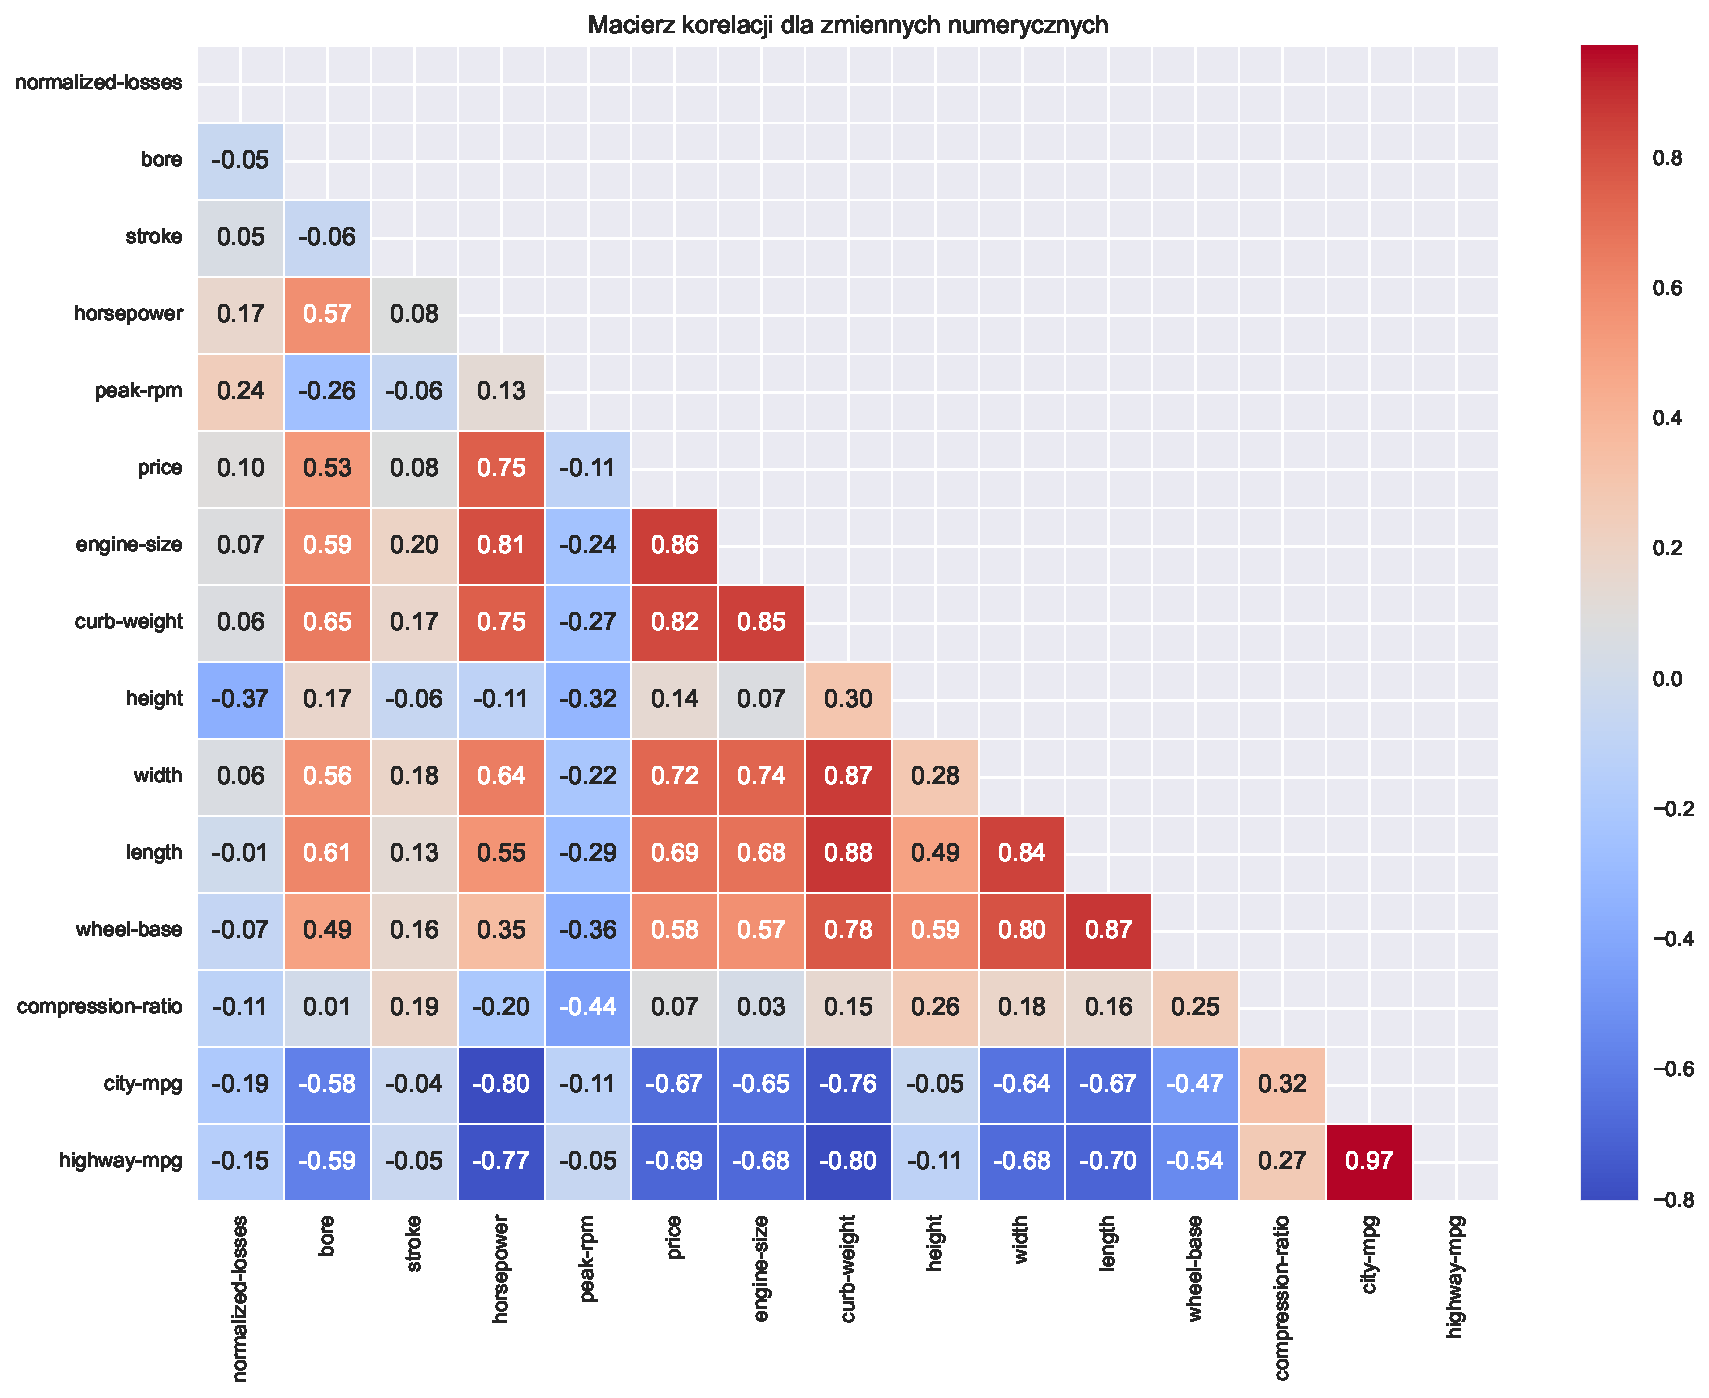
\includegraphics[width=0.9\textwidth]{correlation_heatmap.pdf}
    \caption{Macierz korelacji dla zmiennych numerycznych}
    \label{fig:correlation_matrix}
    \small\textit{Mapa ciepła obrazująca współczynniki korelacji między zmiennymi numerycznymi. Intensywność koloru odpowiada sile korelacji, od ciemnoniebieskiego (silna ujemna korelacja) przez biały (brak korelacji) do ciemnoczerwonego (silna dodatnia korelacja).}
\end{figure}

Analiza macierzy korelacji wykazała silne zależności pomiędzy niektórymi zmiennymi:
\begin{itemize}
    \item Silna dodatnia korelacja między \texttt{engine-size} a \texttt{horsepower} (r ≈ 0.8), co jest zgodne z oczekiwaniami technicznymi.
    
    \item Silna ujemna korelacja między \texttt{horsepower} a \texttt{city-mpg} (r ≈ -0.7), wskazująca na kompromis między mocą silnika a ekonomią spalania.
    
    \item Bardzo silna dodatnia korelacja między \texttt{city-mpg} a \texttt{highway-mpg} (r > 0.9), co wskazuje na spójność tych miar efektywności paliwowej.
\end{itemize}

\begin{figure}[H]
    \centering
    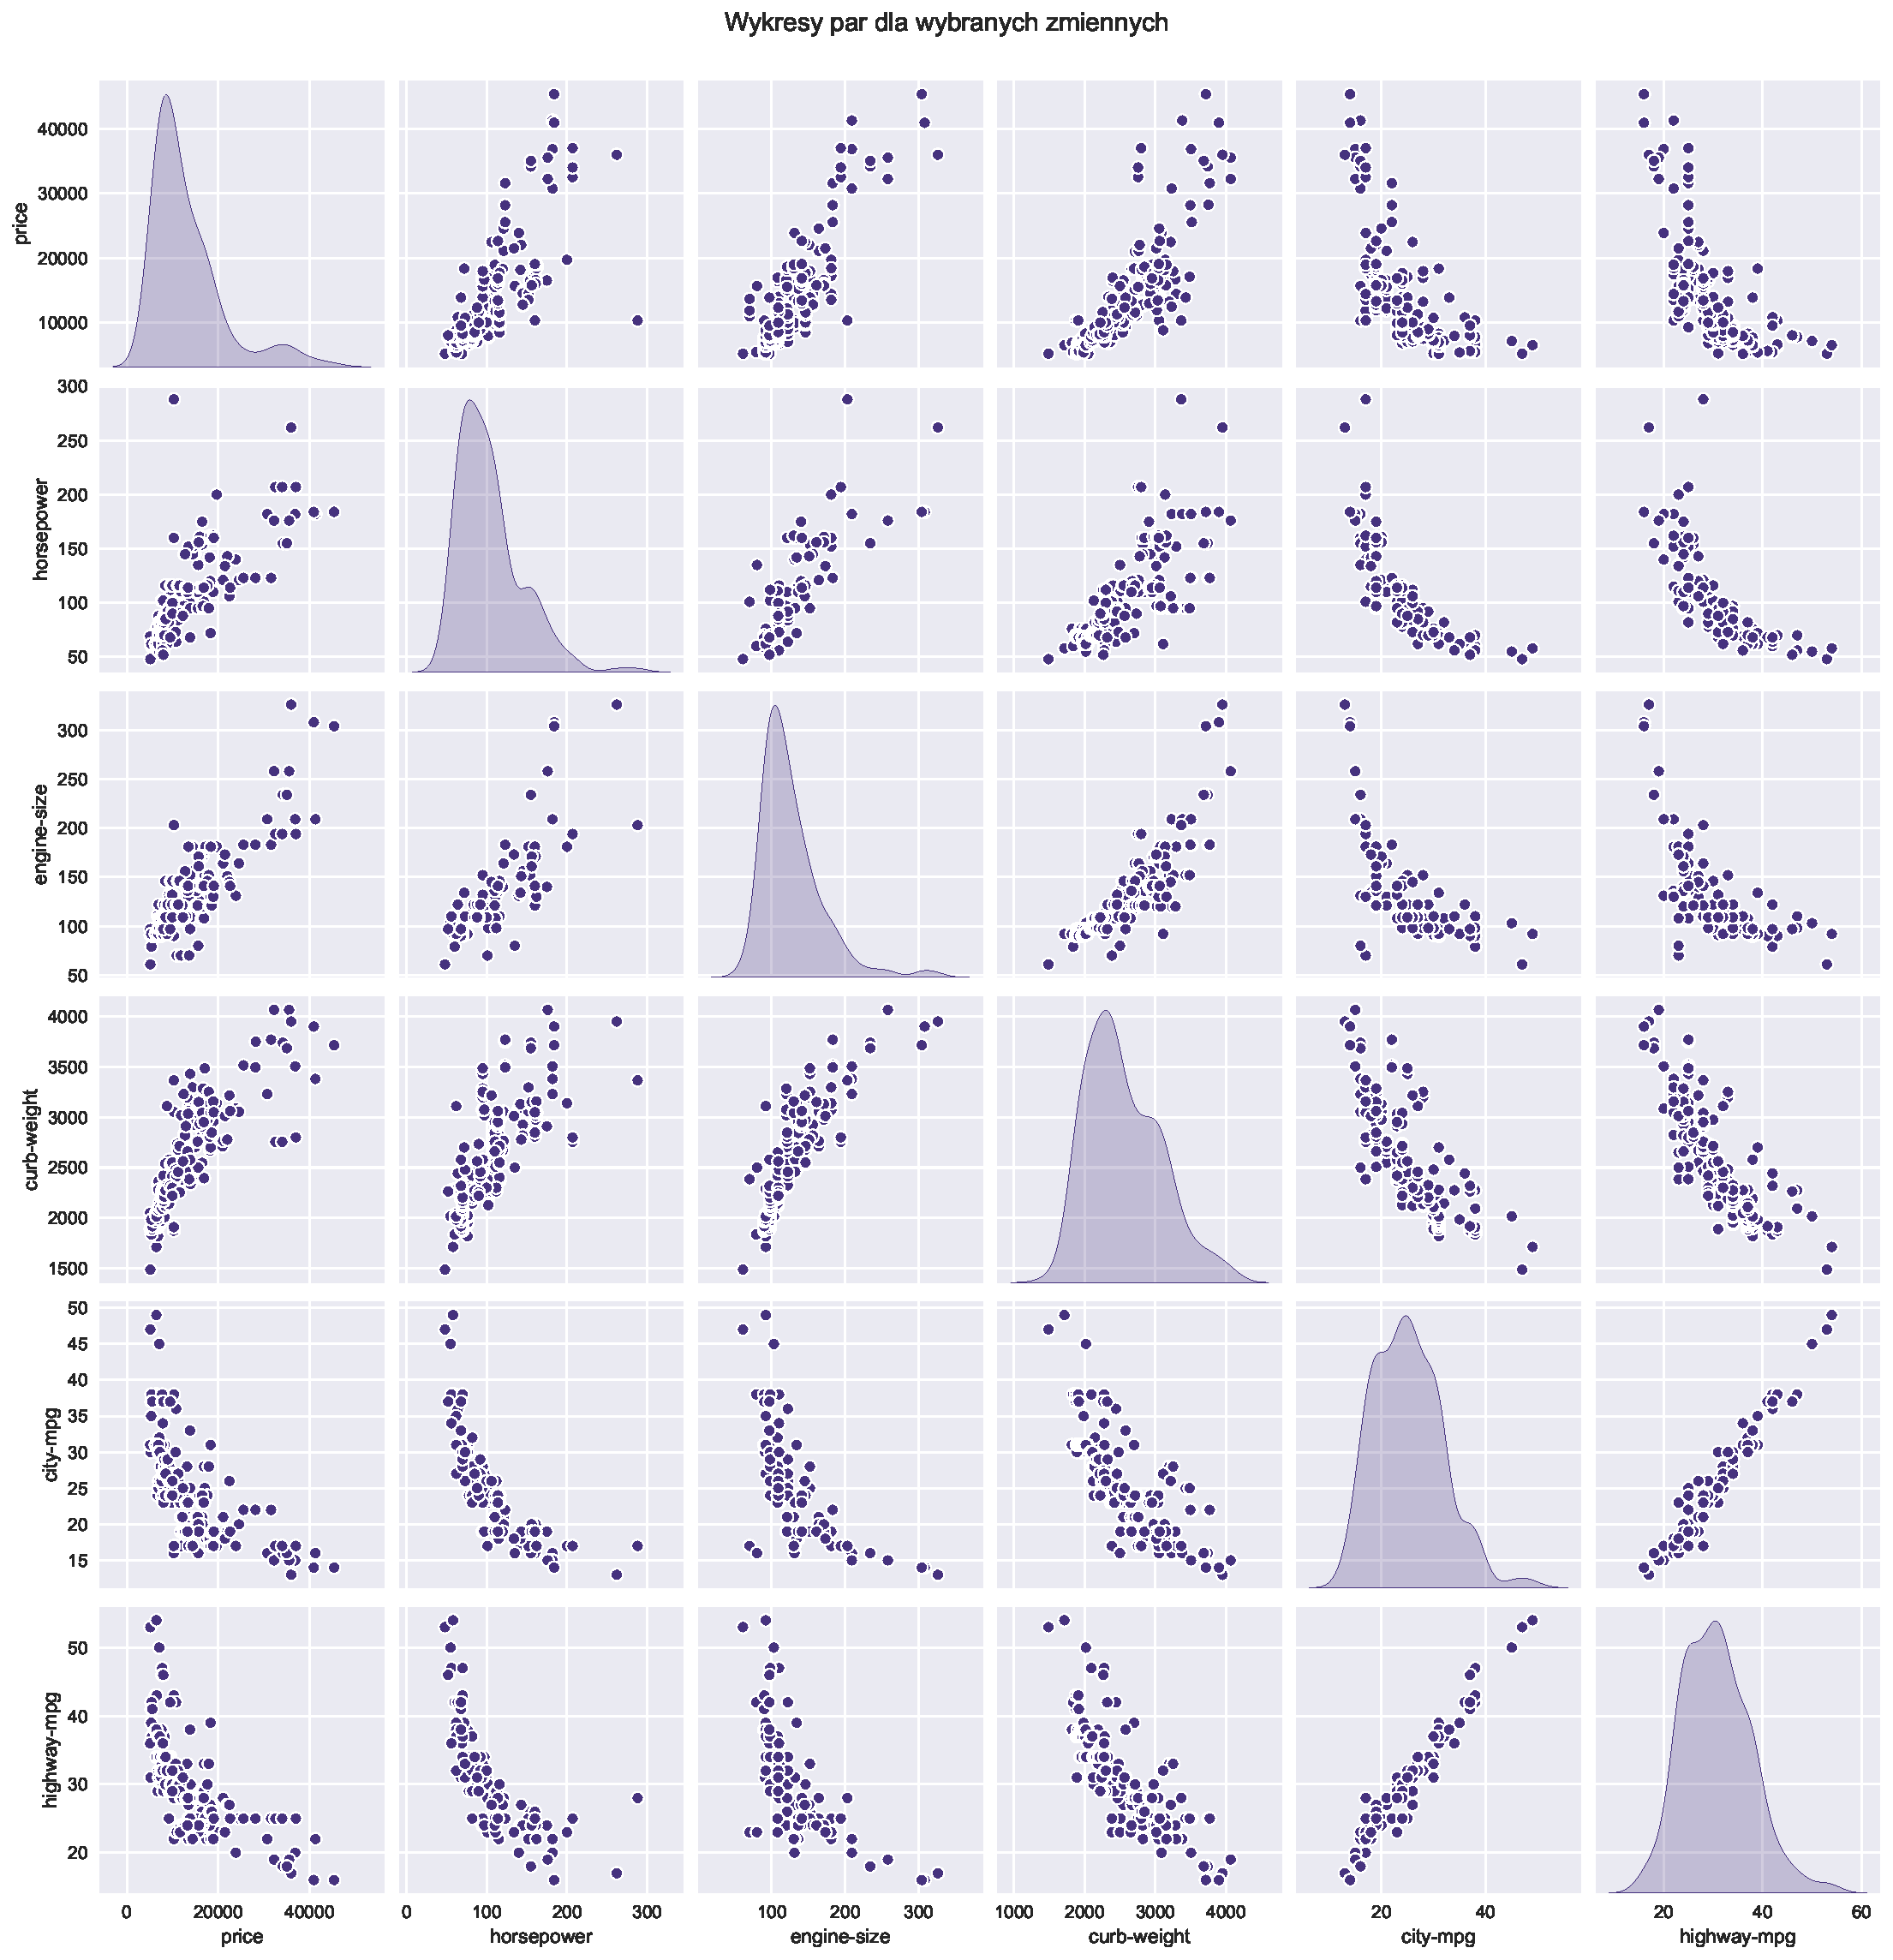
\includegraphics[width=0.95\textwidth]{pairplot_matrix.pdf}
    \caption{Macierz wykresów par dla wybranych zmiennych}
    \label{fig:pairplot_matrix}
    \small\textit{Macierz wykresów par przedstawiająca zależności między wybranymi zmiennymi. Na przekątnej znajdują się wykresy gęstości KDE, poza przekątną wykresy rozproszenia. Widoczne są m.in. silne zależności liniowe między pojemnością silnika a jego mocą oraz między zużyciem paliwa w mieście i na autostradzie.}
\end{figure}

\subsection{Wykresy rozproszenia}

Wykresy rozproszenia z podziałem na kategorie (np. typ nadwozia) uwidoczniły zależności między zmiennymi ciągłymi a kategorialnymi. Na przykład, dla zmiennych \texttt{horsepower} i \texttt{price} zaobserwowano grupowanie się samochodów sportowych w obszarze wysokiej mocy i wysokiej ceny.

\begin{figure}[H]
    \centering
    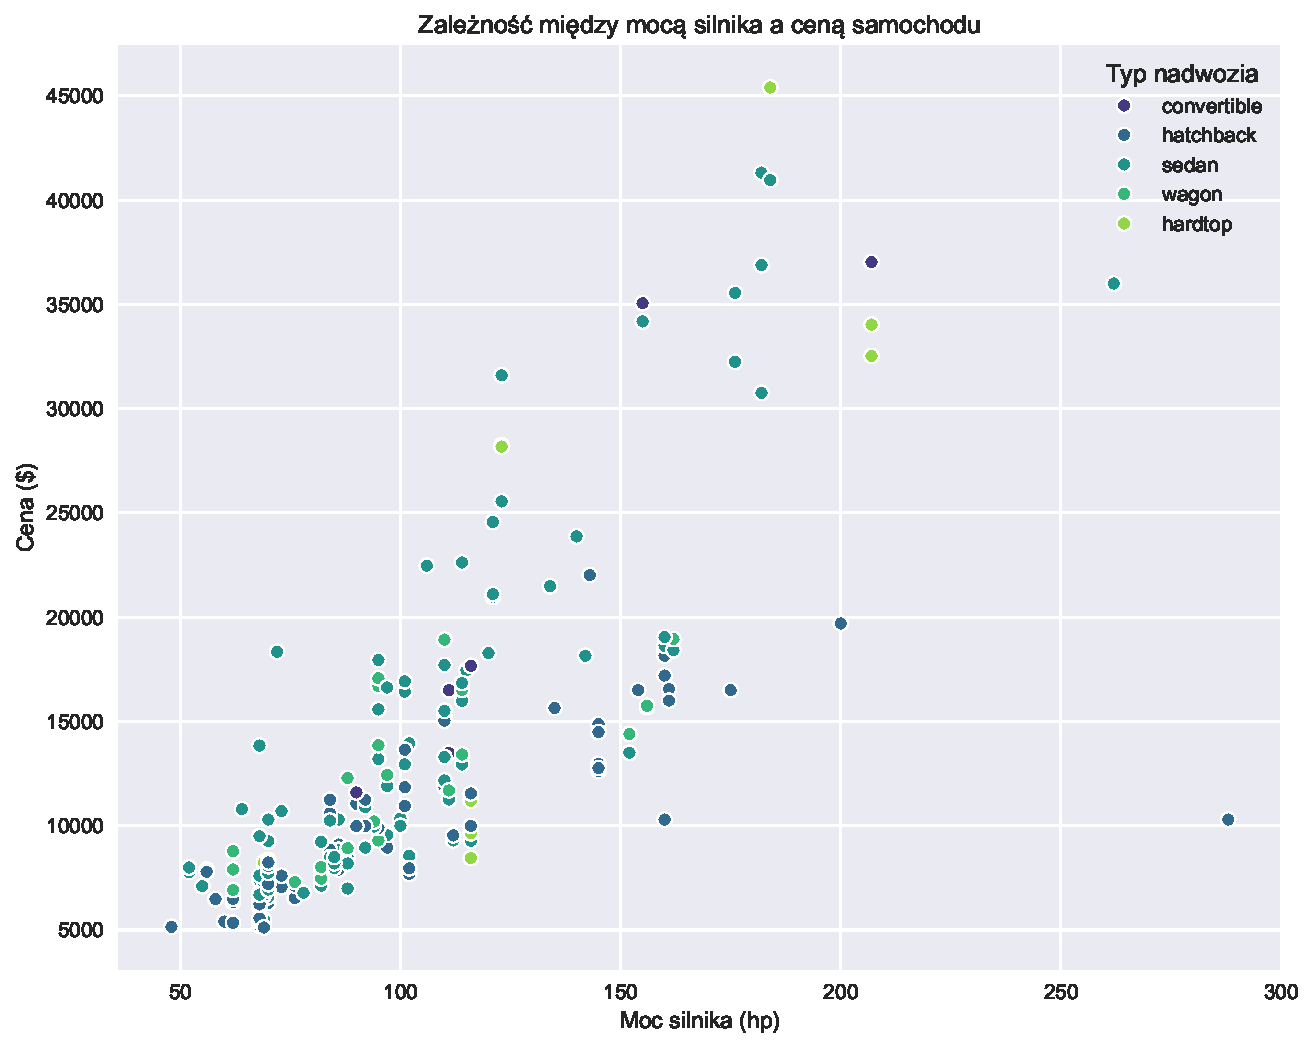
\includegraphics[width=0.85\textwidth]{scatter_hp_price_by_body.pdf}
    \caption{Wykres rozproszenia mocy silnika i ceny według typu nadwozia}
    \label{fig:scatter_by_category}
    \small\textit{Wykres rozproszenia pokazujący zależność między mocą silnika (hp) a ceną samochodu, z podziałem na typy nadwozia. Widoczne jest grupowanie się poszczególnych kategorii w różnych obszarach wykresu, co wskazuje na zależność ceny i mocy od typu nadwozia.}
\end{figure}

\begin{figure}[H]
    \centering
    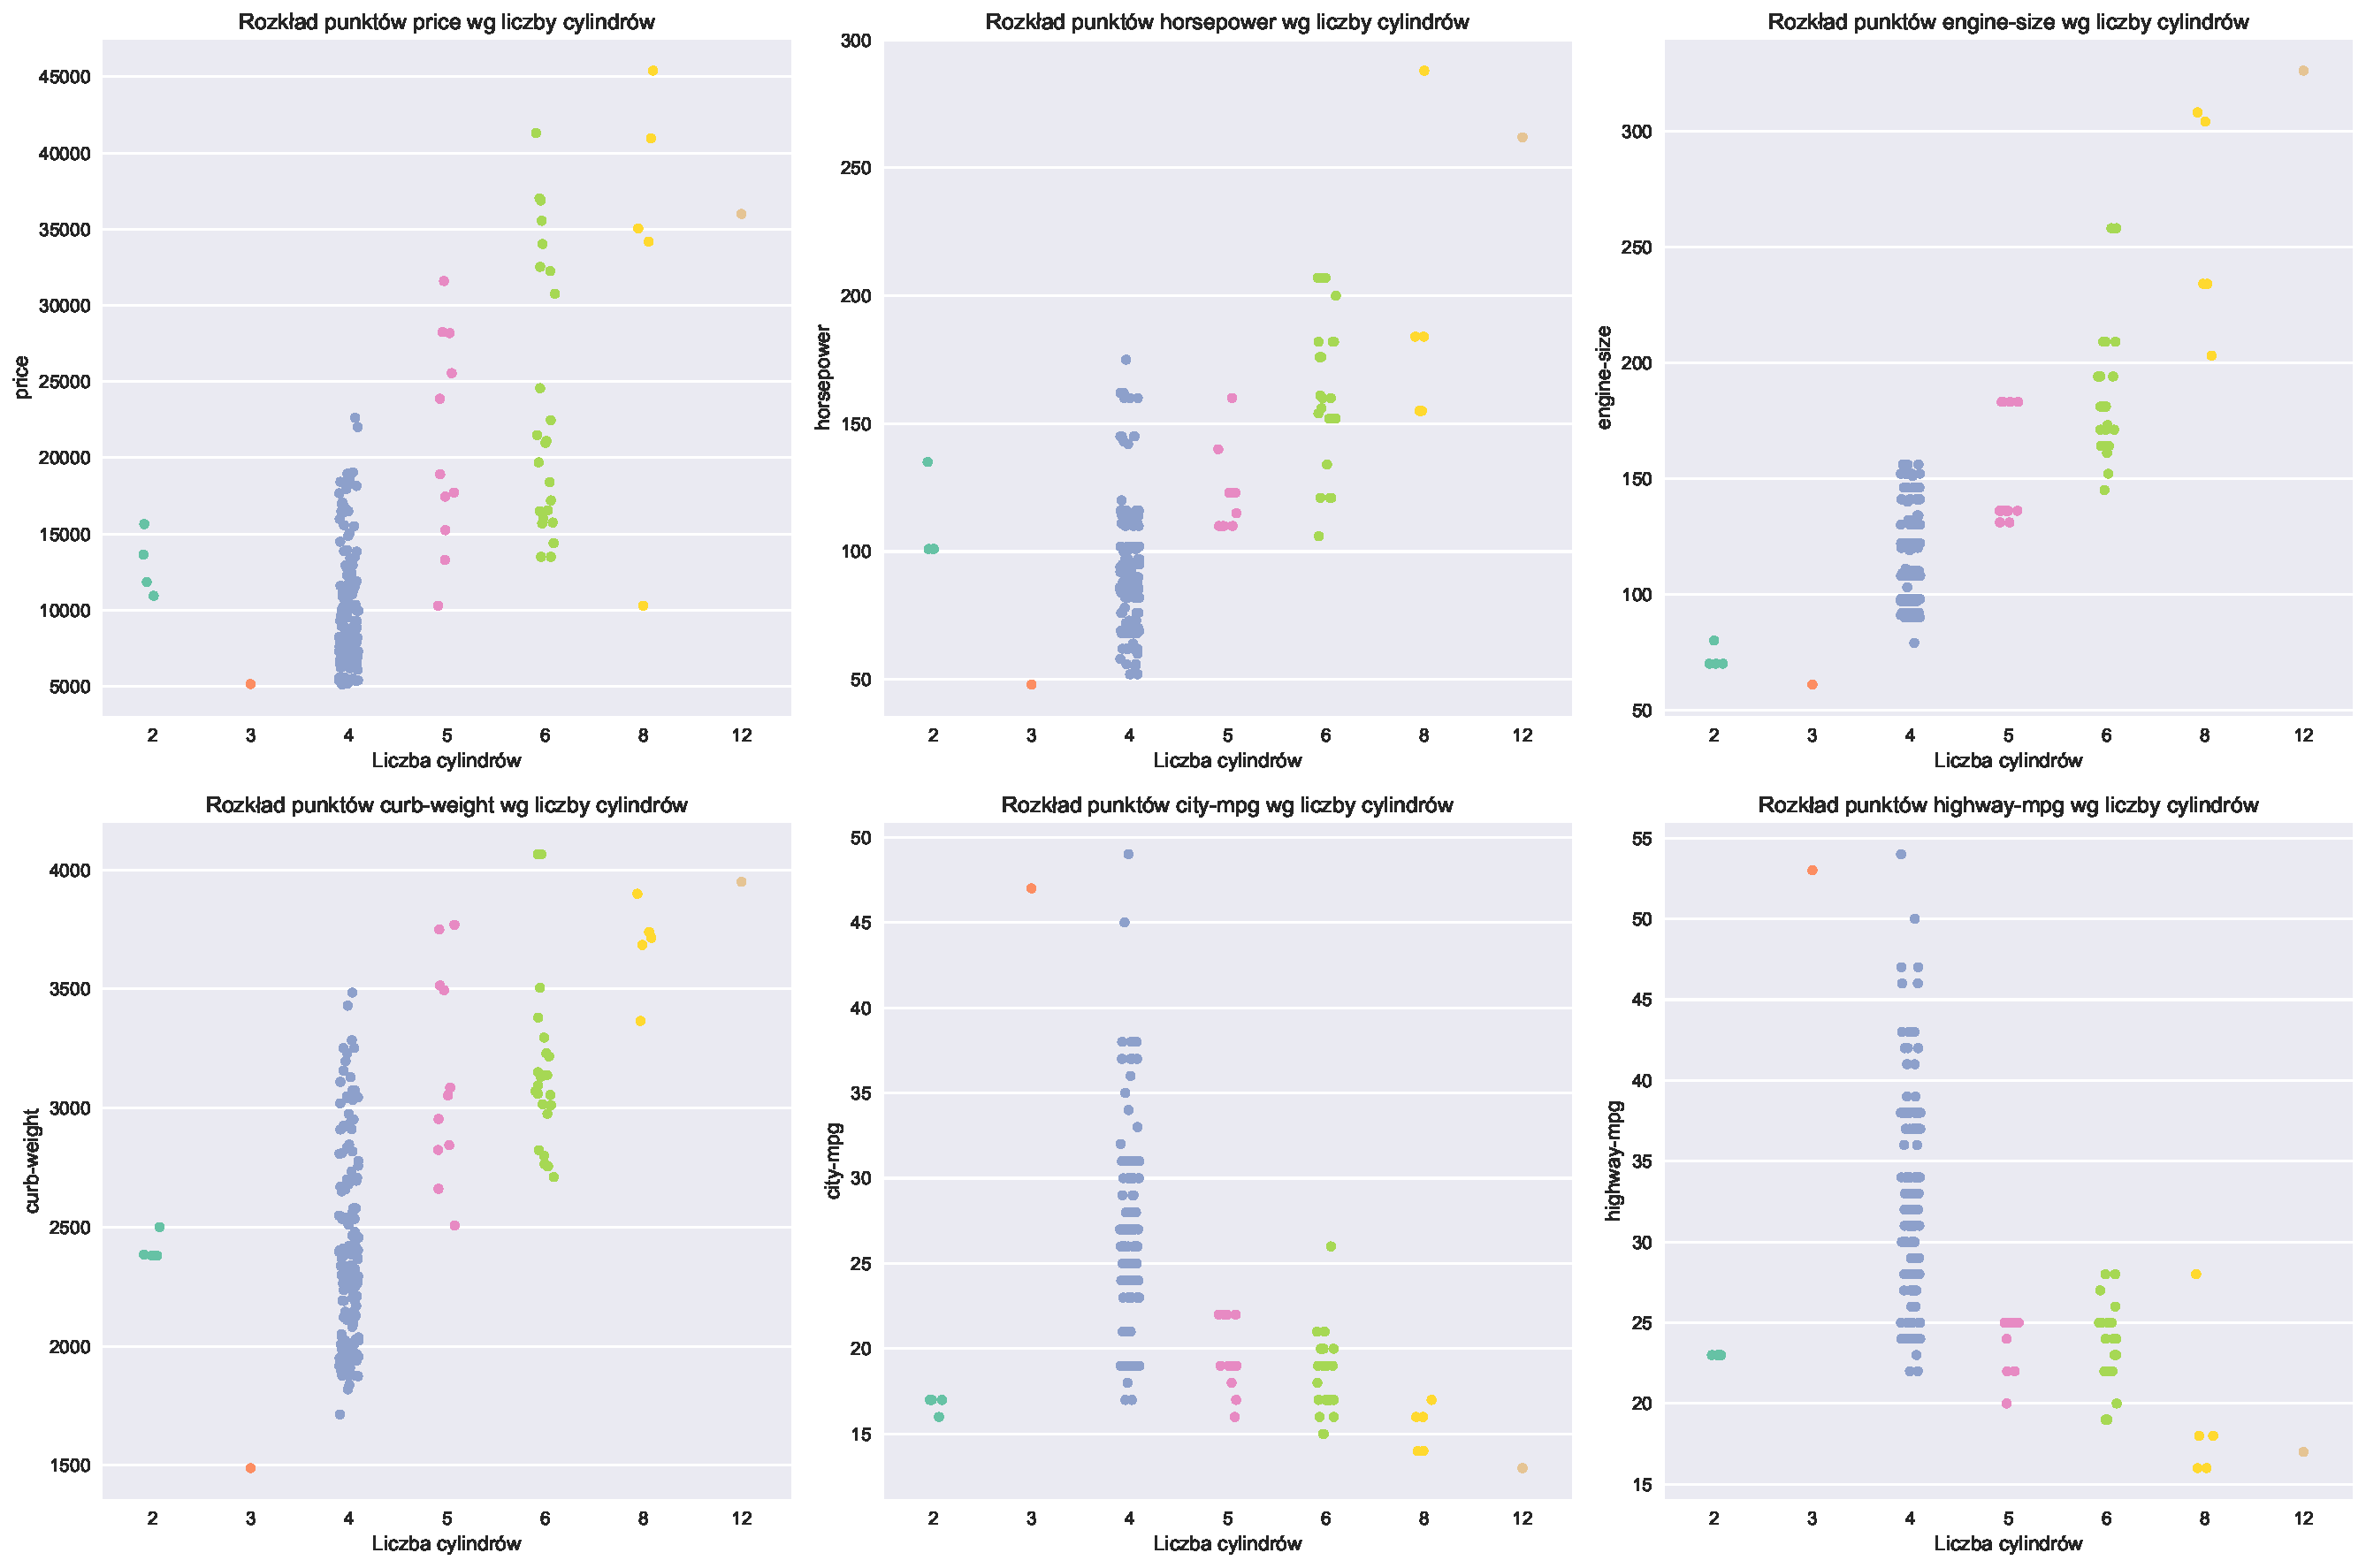
\includegraphics[width=0.95\textwidth]{strip_plots_by_cylinder.pdf}
    \caption{Wykresy rozrzutu punktowego według liczby cylindrów}
    \label{fig:strip_plots}
    \small\textit{Wykresy rozrzutu punktowego pokazujące rozkład wartości zmiennych numerycznych w zależności od liczby cylindrów silnika. Pozwala to na analizę wpływu liczby cylindrów na inne parametry pojazdu.}
\end{figure}

\section{Testy normalności rozkładów}

Aby formalnie ocenić, czy analizowane zmienne podlegają rozkładowi normalnemu, przeprowadzono trzy różne testy statystyczne.

\kod{
import matplotlib.pyplot as plt
import seaborn as sns
from scipy import stats
import pandas as pd

shapiro_p_values = []
dagostino_p_values = []
anderson_results = []

for var in continuous_vars:
    data = df[var].dropna()
    
    # Test Shapiro-Wilka
    _, shapiro_p = stats.shapiro(data)
    shapiro_p_values.append(shapiro_p)
    
    # Test D'Agostino-Pearsona
    _, dagostino_p = stats.normaltest(data)
    dagostino_p_values.append(dagostino_p)
    
    # Test Andersona-Darlinga
    anderson_result = stats.anderson(data, dist='norm')
    anderson_results.append(anderson_result.statistic)

# Utworzenie DataFrame z wynikami testów
normality_tests = pd.DataFrame({
    'Variable': continuous_vars,
    'Shapiro_p': shapiro_p_values,
    'DAgostino_p': dagostino_p_values,
    'Anderson_stat': anderson_results
})
normality_tests.to_csv('figures/normality_tests.csv', index=False)

# Wizualizacja wyników testów normalności
fig_norm, axes = plt.subplots(1, 3, figsize=(16, 8))

axes[0].bar(continuous_vars, shapiro_p_values, color='#00F')
axes[0].axhline(y=0.05, color='red', linestyle='--', label='Poziom istotności (0.05)')
axes[0].set_title('p-wartości testu Shapiro-Wilka')
axes[0].set_ylabel('p-wartość')
axes[0].set_xticks(range(len(continuous_vars)))
axes[0].set_xticklabels(continuous_vars, rotation=45)
axes[0].legend()

axes[1].bar(continuous_vars, dagostino_p_values, color='#0F0')
axes[1].axhline(y=0.05, color='red', linestyle='--', label='Poziom istotności (0.05)')
axes[1].set_title('p-wartości testu D\'Agostino-Pearsona')
axes[1].set_ylabel('p-wartość')
axes[1].set_xticks(range(len(continuous_vars)))
axes[1].set_xticklabels(continuous_vars, rotation=45)
axes[1].legend()

axes[2].bar(continuous_vars, anderson_results, color='orange')
axes[2].set_title('Statystyka testu Andersona-Darlinga')
axes[2].set_ylabel('Wartość statystyki')
axes[2].set_xticks(range(len(continuous_vars)))
axes[2].set_xticklabels(continuous_vars, rotation=45)

plt.tight_layout()
save_fig(fig_norm, 'normality_tests', directory='figures')
plt.show()
}{Kod wykonujący testy normalności: Shapiro-Wilka, D'Agostino-Pearsona i Andersona-Darlinga}

\begin{figure}[H]
    \centering
    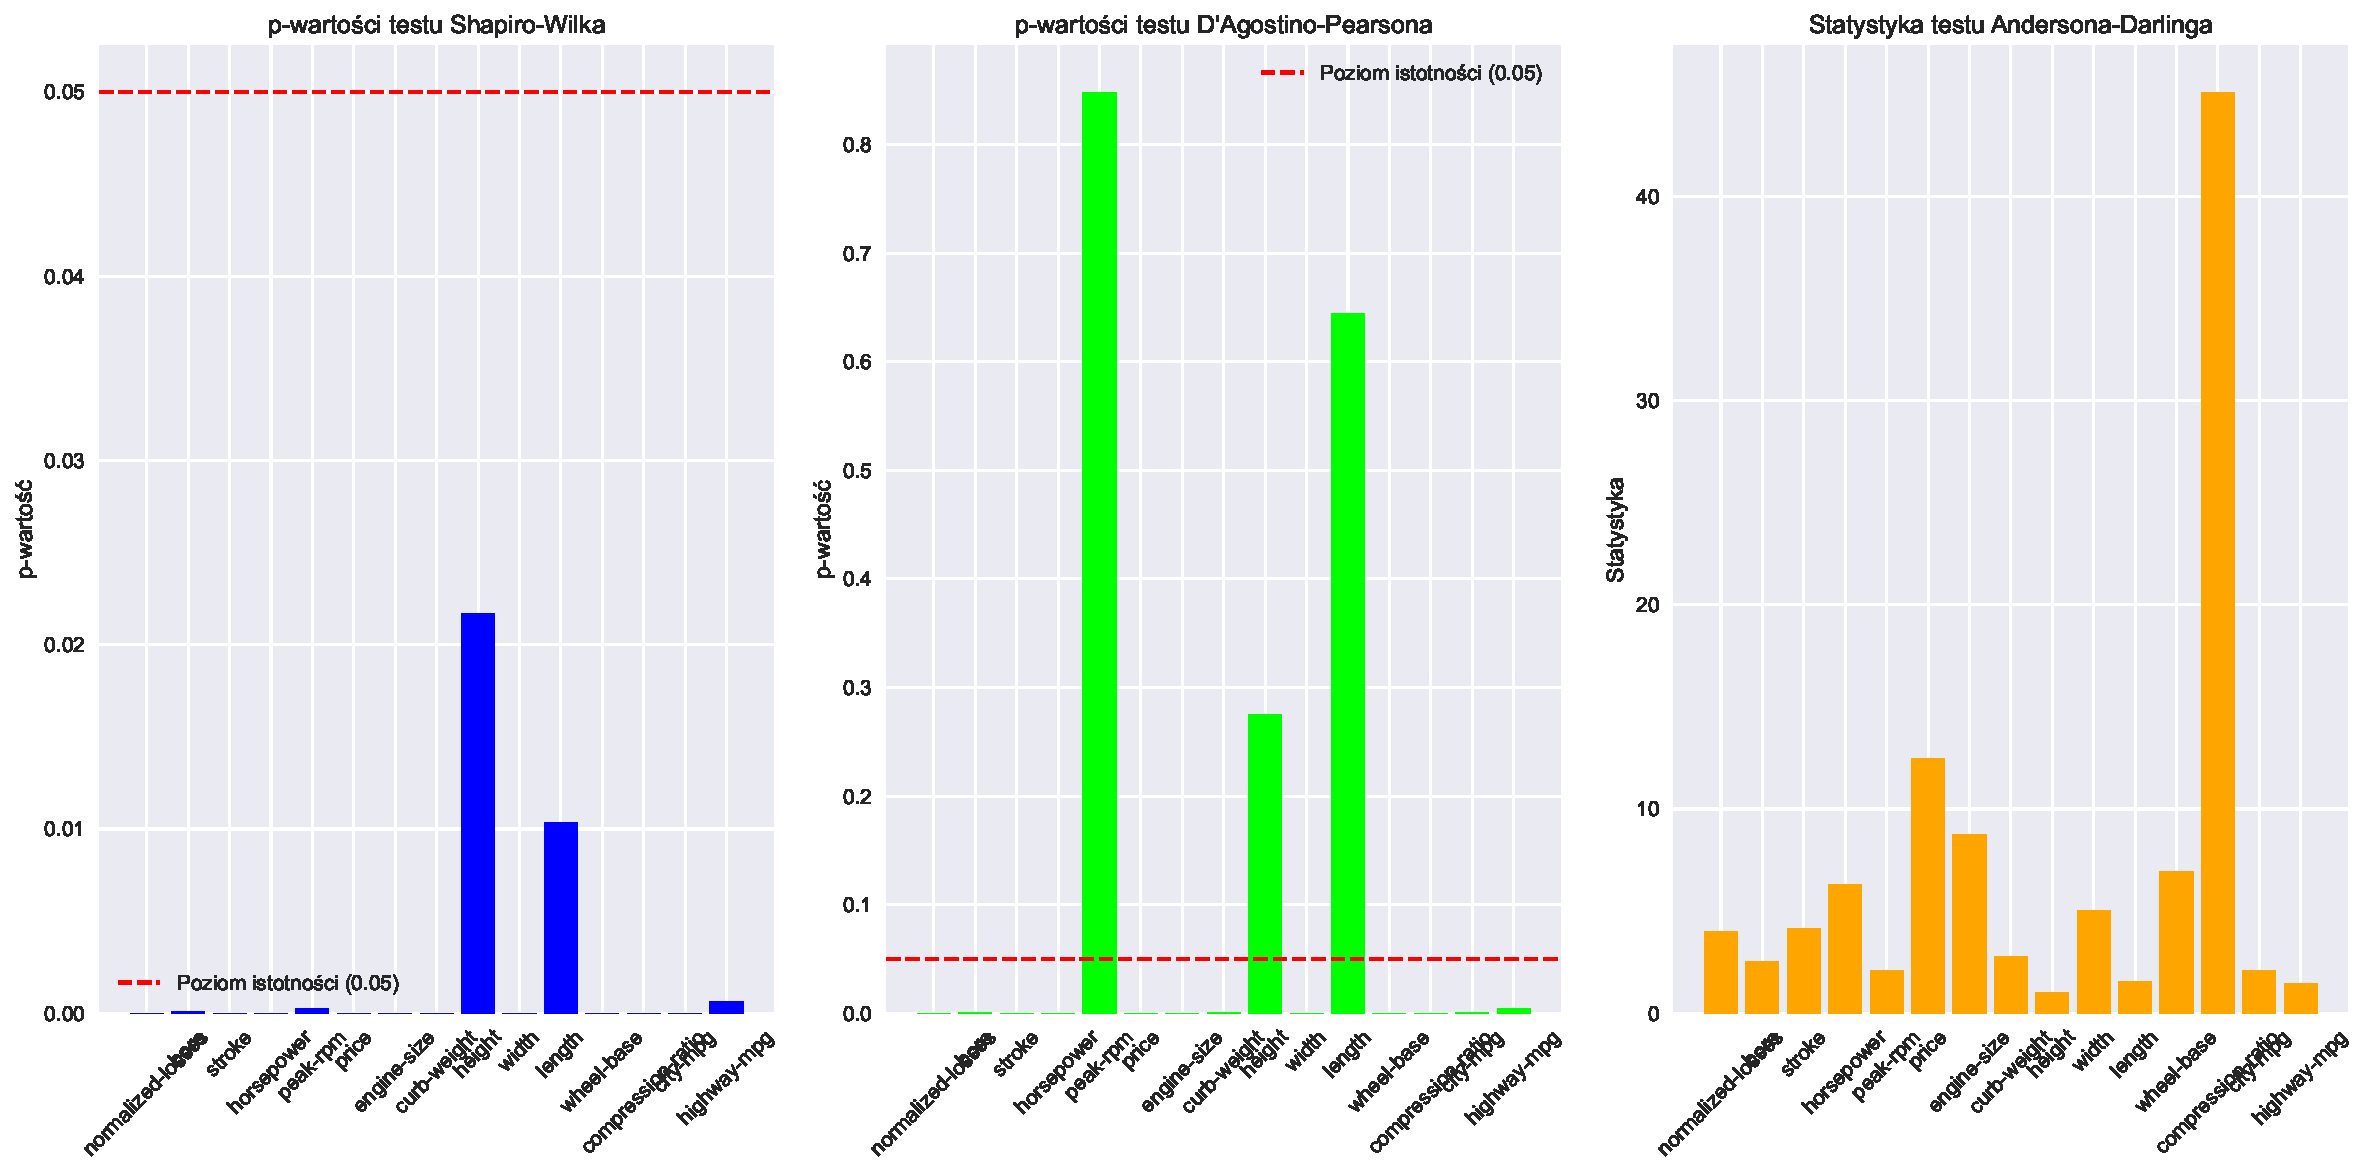
\includegraphics[width=0.95\textwidth]{normality_tests.pdf}
    \caption{Wyniki testów normalności dla zmiennych ciągłych}
    \label{fig:normality_tests}
    \small\textit{Wykres przedstawia rezultaty trzech testów normalności: Shapiro-Wilka, D'Agostino-Pearsona oraz Andersona-Darlinga. Dla dwóch pierwszych testów pokazano p-wartości (czerwona linia oznacza poziom istotności 0.05), dla trzeciego przedstawiono wartości statystyki testowej (większa wartość oznacza silniejsze odchylenie od rozkładu normalnego).}
\end{figure}

\subsection{Test Shapiro-Wilka}

Test ten uważany jest za jeden z najsilniejszych testów normalności, szczególnie dla małych i średnich próbek.

Wyniki testu Shapiro-Wilka wykazały, że dla żadnej z badanych zmiennych p-wartość nie przekroczyła poziomu istotności α = 0.05, co oznacza, że dla wszystkich zmiennych należy odrzucić hipotezę o normalności rozkładu.

\subsection{Test D'Agostino-Pearsona}

Ten test łączy informację o skośności i kurtozie w celu oceny normalności.

Wyniki testu D'Agostino-Pearsona wskazały, że tylko dwie zmienne (\texttt{horsepower} i \texttt{width}) miały p-wartość wyraźnie przekraczającą 0.05, co oznacza brak podstaw do odrzucenia hipotezy o normalności dla tych zmiennych.

\subsection{Test Andersona-Darlinga}

Test ten kładzie większy nacisk na ogony rozkładu.

Najwyższą statystyką testu Andersona-Darlinga charakteryzowała się zmienna \texttt{compression-ratio} (statystyka ≈ 45), co wskazuje na znaczne odstępstwo od rozkładu normalnego. Najniższe wartości statystyki zaobserwowano dla zmiennych \texttt{height}, \texttt{curb-weight} i \texttt{engine-size}.

\subsection{Wnioski z testów normalności}

Na podstawie przeprowadzonych testów można stwierdzić, że:
\begin{itemize}
    \item Większość zmiennych w zbiorze danych nie pochodzi z rozkładu normalnego.
    
    \item Tylko nieliczne zmienne (\texttt{horsepower}, \texttt{width}) mogą być rozpatrywane jako zbliżone do rozkładu normalnego.
    
    \item Przed zastosowaniem metod statystycznych zakładających normalność (np. testy parametryczne) zaleca się przeprowadzenie transformacji danych, np. transformacji logarytmicznej lub standaryzacji.
\end{itemize}

\section{Testy statystyczne dla średniej i wariancji}

W celu oceny właściwości statystycznych analizowanych zmiennych przeprowadzono testy dla średniej i wariancji.

\kod{
# Test t-Studenta dla średniej
t_stats = []
p_values_t = []

for var in continuous_vars:
    data = df[var].dropna()
    t_stat, p_value = stats.ttest_1samp(data, 0)
    t_stats.append(t_stat)
    p_values_t.append(p_value)

# Create DataFrame with test results
stat_tests = pd.DataFrame({
    'Variable': continuous_vars,
    't_stat': t_stats,
    't_pvalue': p_values_t
})

# T-test statistics plot
fig_t_stat = plt.figure(figsize=(12, 6))
plt.bar(continuous_vars, t_stats, color='skyblue')
plt.axhline(y=0, color='red', linestyle='--', label='Linia odniesienia (t=0)')
plt.title('Wyniki testu t-Studenta dla średniej', fontsize=14)
plt.ylabel('Statystyka t')
plt.xticks(rotation=45)
plt.legend()
plt.tight_layout()
save_fig(fig_t_stat, 't_test_statistics', directory='figures')
plt.show()

# T-test p-values plot
fig_t_pval = plt.figure(figsize=(12, 6))
plt.bar(continuous_vars, p_values_t, color='lightgreen')
plt.axhline(y=0.05, color='green', linestyle='--', label='Poziom istotności (0.05)')
plt.title('p-wartości testu t-Studenta dla średniej', fontsize=14)
plt.ylabel('p-wartość')
plt.xticks(rotation=45)
plt.yscale('log')  # Logarytmiczna skala dla lepszej wizualizacji małych p-wartości
plt.legend()
plt.tight_layout()
save_fig(fig_t_pval, 't_test_pvalues', directory='figures')
plt.show()

# Test chi-kwadrat dla wariancji
chi2_stats = []
p_values_chi2 = []

for var in continuous_vars:
    data = df[var].dropna()
    n = len(data)
    dof = n - 1  # stopnie swobody
    sample_var = np.var(data, ddof=1)
    theoretical_var = 1.0  # założona wartość teoretyczna
    
    chi2_stat = dof * sample_var / theoretical_var
    p_value = 1 - stats.chi2.cdf(chi2_stat, dof)  # test jednostronny
    
    chi2_stats.append(chi2_stat)
    p_values_chi2.append(p_value)

# Chi-squared test statistics plot
fig_chi2_stat = plt.figure(figsize=(12, 6))
plt.bar(continuous_vars, np.log10(chi2_stats), color='orange')  # Logarytmiczna skala dla lepszej wizualizacji
plt.title('Statystyka testu chi-kwadrat dla wariancji (skala logarytmiczna)', fontsize=14)
plt.ylabel('log10(Statystyka chi-kwadrat)')
plt.xticks(rotation=45)
plt.tight_layout()
save_fig(fig_chi2_stat, 'chi2_test_statistics', directory='figures')
plt.show()

# Chi-squared test p-values plot
fig_chi2_pval = plt.figure(figsize=(12, 6))
plt.bar(continuous_vars, p_values_chi2, color='pink')
plt.axhline(y=0.05, color='green', linestyle='--', label='Poziom istotności (0.05)')
plt.title('p-wartości testu chi-kwadrat dla wariancji', fontsize=14)
plt.ylabel('p-wartość')
plt.xticks(rotation=45)
plt.yscale('log')  # Logarytmiczna skala dla lepszej wizualizacji małych p-wartości
plt.legend()
plt.tight_layout()
save_fig(fig_chi2_pval, 'chi2_test_pvalues', directory='figures')
plt.show()
}{Kod wykonujący testy statystyczne dla średniej (test t-Studenta) i wariancji (test chi-kwadrat)}

\subsection{Test t-Studenta dla średniej}

Dla każdej zmiennej przeprowadzono jednoetapowy test t-Studenta, weryfikujący hipotezę zerową, że średnia zmiennej wynosi 0.

\begin{figure}[H]
    \centering
    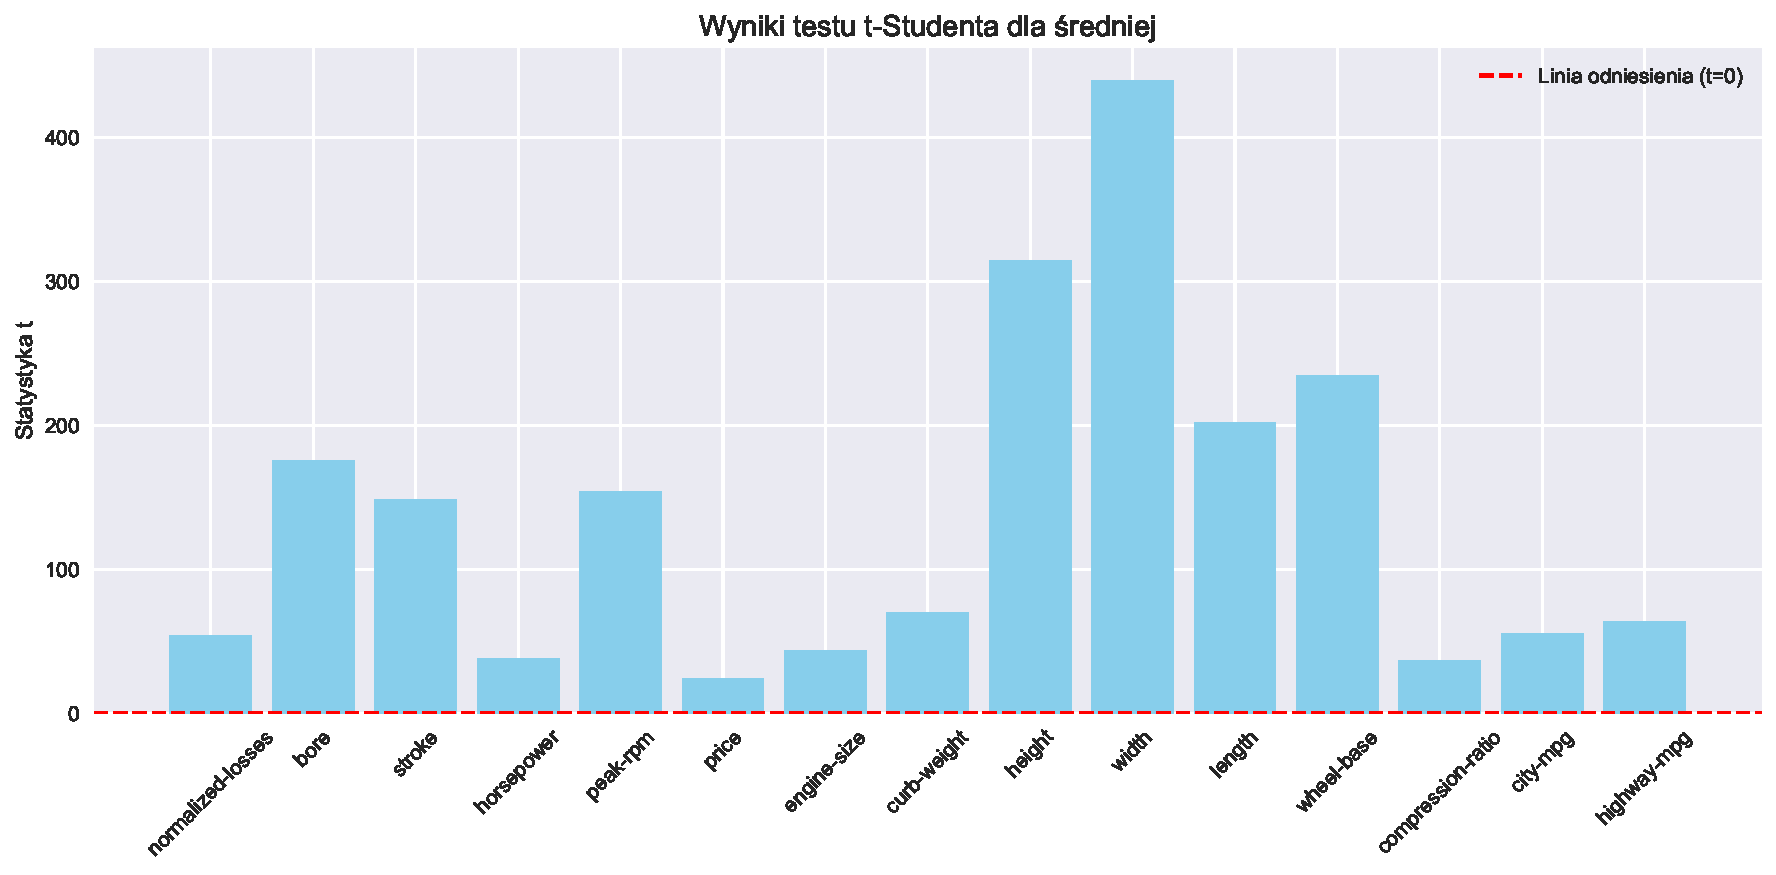
\includegraphics[width=0.9\textwidth]{t_test_statistics.pdf}
    \caption{Wartości statystyki t-Studenta dla średniej}
    \label{fig:t_test_stat}
    \small\textit{Wykres przedstawia wartości statystyki t-Studenta dla testu weryfikującego hipotezę zerową, że średnie zmiennych są równe zero. Czerwona linia przerywana oznacza wartość odniesienia (t=0). Wysokie wartości statystyki t dla większości zmiennych wskazują na istotne odchylenia średnich od zera.}
\end{figure}

\begin{figure}[H]
    \centering
    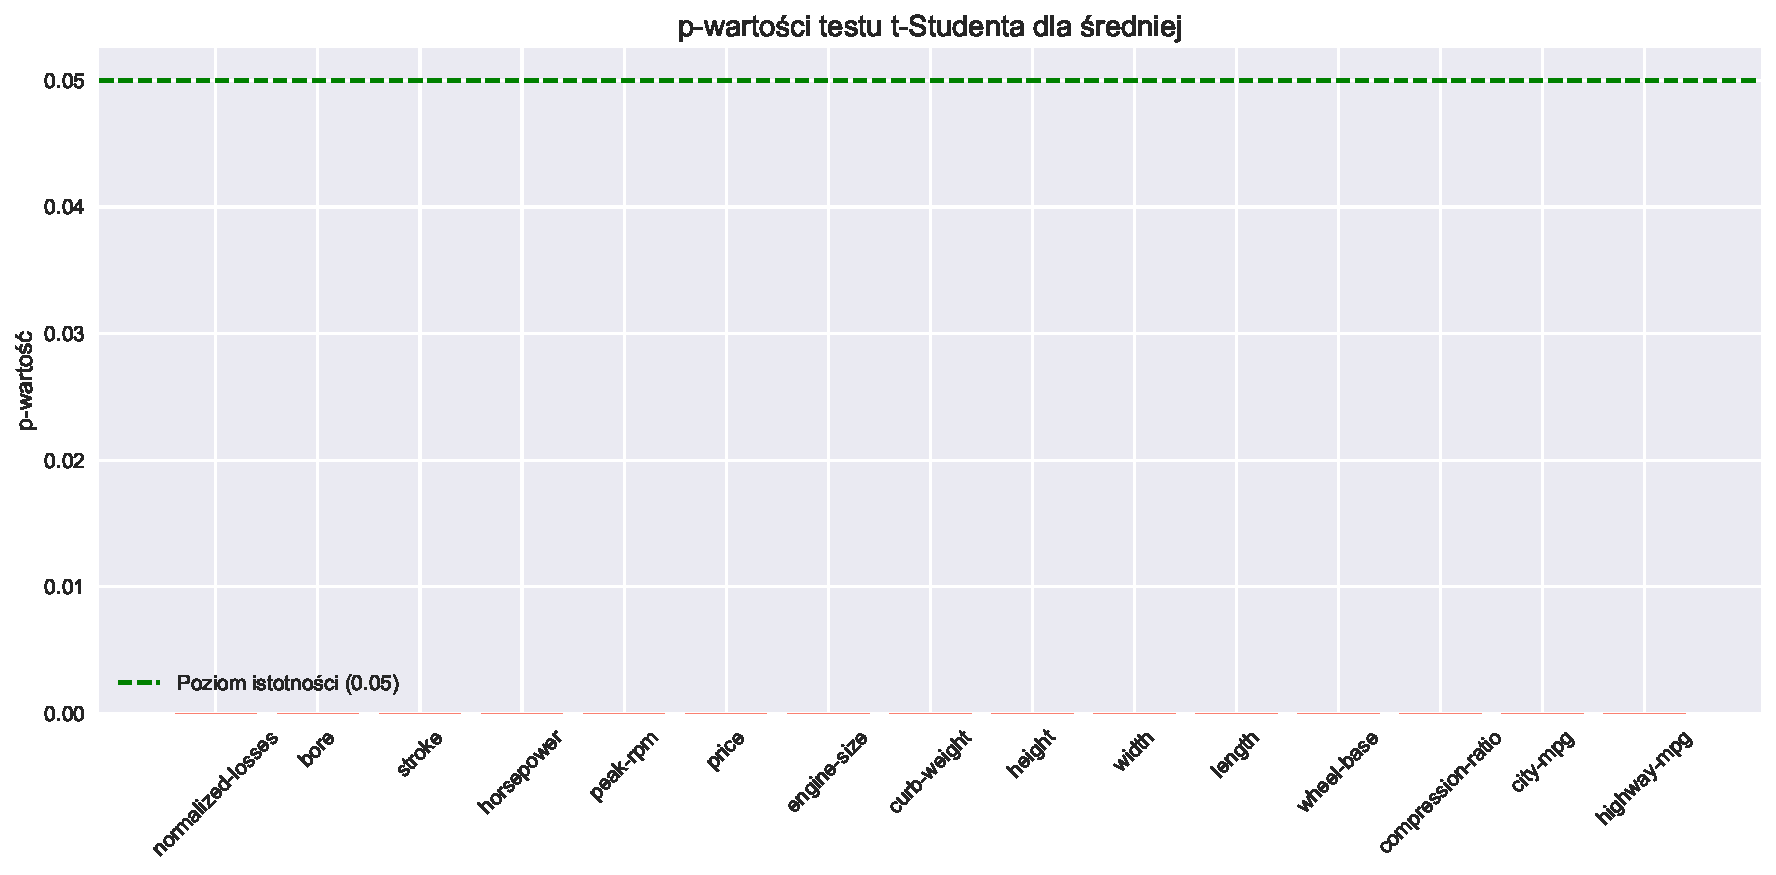
\includegraphics[width=0.9\textwidth]{t_test_pvalues.pdf}
    \caption{p-wartości testu t-Studenta dla średniej}
    \label{fig:t_test_pval}
    \small\textit{Wykres przedstawia p-wartości testu t-Studenta. Zielona linia przerywana oznacza poziom istotności 0.05. Wszystkie p-wartości są znacznie niższe od tego poziomu, co oznacza odrzucenie hipotezy zerowej o równości średnich z zerem.}
\end{figure}

Wyniki testu wykazały, że dla wszystkich zmiennych p-wartości były znacznie poniżej poziomu istotności 0.05, co oznacza, że średnie wszystkich zmiennych są istotnie różne od zera. Szczególnie wysokie statystyki t zaobserwowano dla cech takich jak \texttt{width}, \texttt{height}, \texttt{wheel-base} i \texttt{length}.

\subsection{Test chi-kwadrat dla wariancji}

Przeprowadzono również test chi-kwadrat, weryfikujący hipotezę zerową, że wariancja zmiennej jest równa wartości teoretycznej (przyjęto wartość 1 jako odniesienie).

\begin{figure}[H]
    \centering
    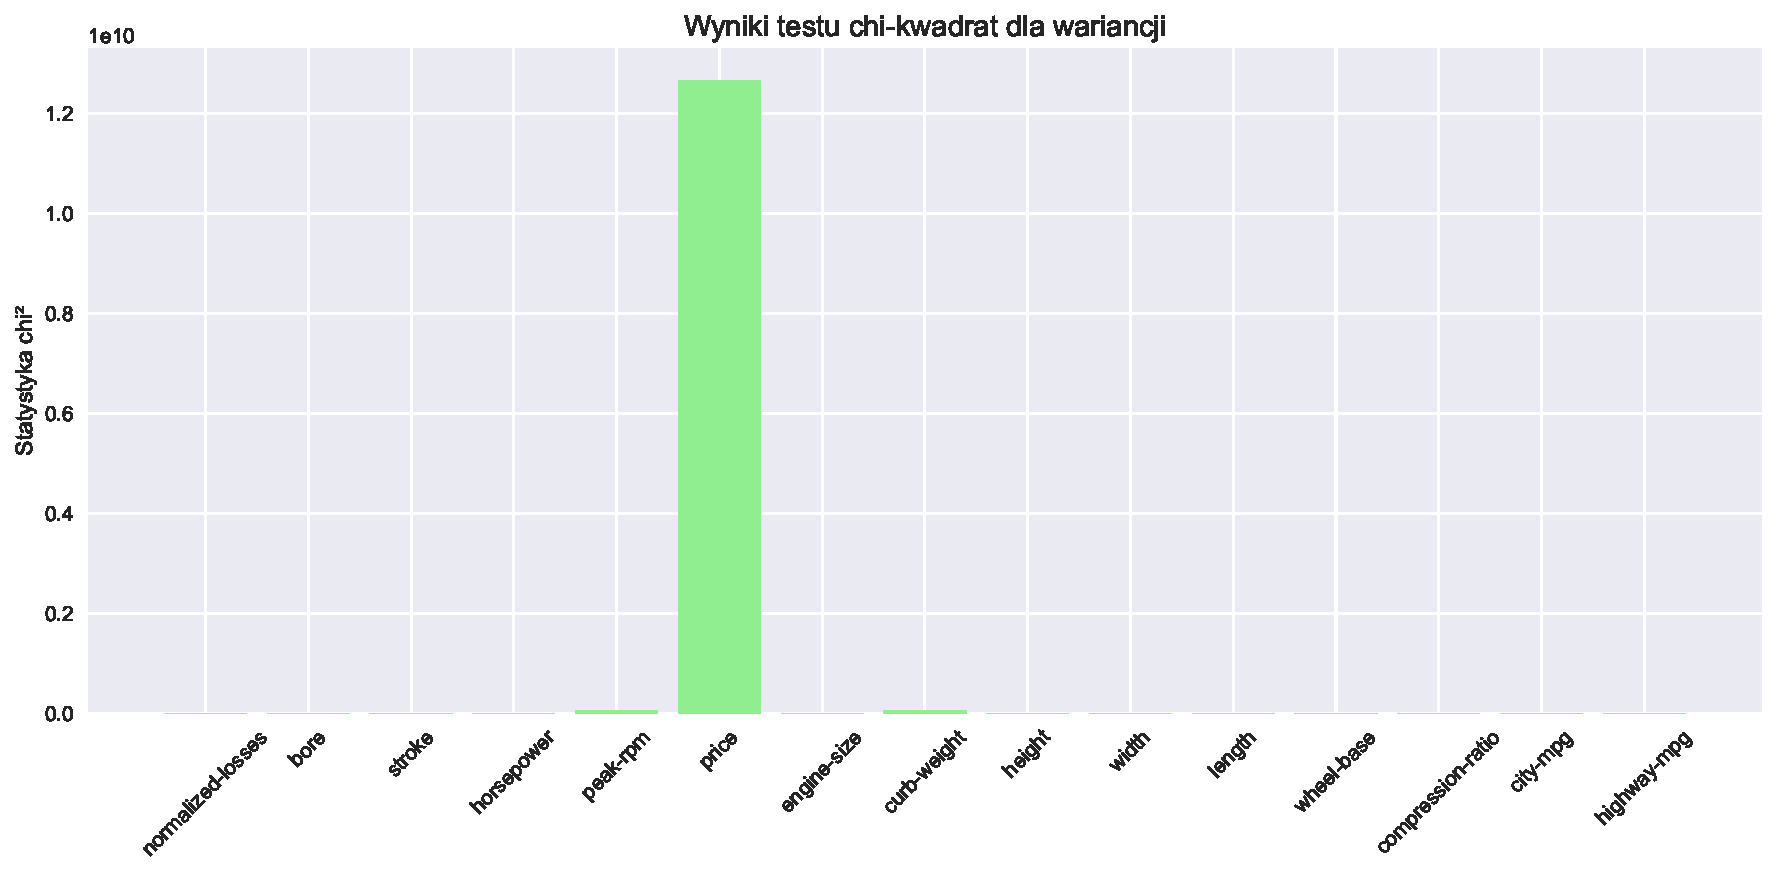
\includegraphics[width=0.9\textwidth]{chi2_test_statistics.pdf}
    \caption{Wartości statystyki chi-kwadrat dla wariancji}
    \label{fig:chi2_test_stat}
    \small\textit{Wykres przedstawia wartości statystyki chi-kwadrat dla testu wariancji. Szczególnie wyróżnia się zmienna \texttt{price} z bardzo wysoką statystyką, co wskazuje na znaczną zmienność cen samochodów.}
\end{figure}

\begin{figure}[H]
    \centering
    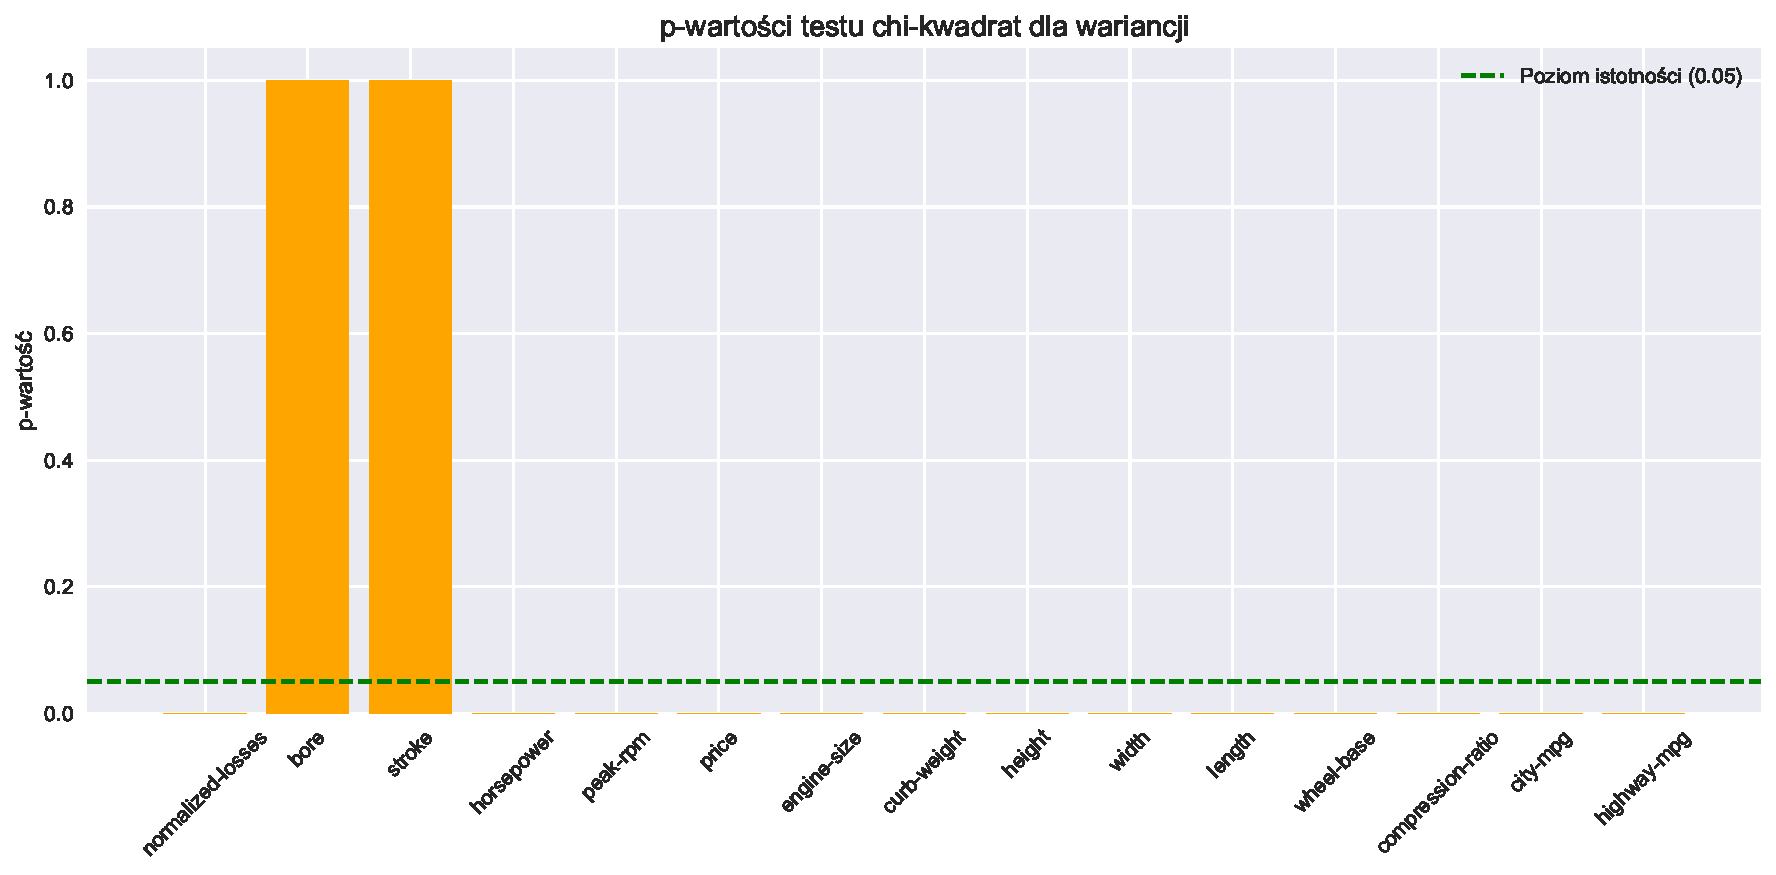
\includegraphics[width=0.9\textwidth]{chi2_test_pvalues.pdf}
    \caption{p-wartości testu chi-kwadrat dla wariancji}
    \label{fig:chi2_test_pval}
    \small\textit{Wykres przedstawia p-wartości testu chi-kwadrat dla wariancji. Zielona linia przerywana oznacza poziom istotności 0.05. Większość zmiennych ma p-wartości poniżej tego poziomu, co oznacza istotną różnicę wariancji od wartości teoretycznej.}
\end{figure}

Większość zmiennych wykazała p-wartości poniżej poziomu istotności 0.05, co oznacza, że ich wariancje różnią się istotnie od wartości teoretycznej. Wyjątkiem były zmienne \texttt{bore} i \texttt{stroke}, których p-wartości były bliskie 1, co wskazuje na brak podstaw do odrzucenia hipotezy zerowej.

\subsection{Interpretacja wyników testów}

Na podstawie przeprowadzonych testów możemy stwierdzić, że:
\begin{itemize}
    \item Średnie wszystkich zmiennych są istotnie różne od zera, co potwierdza ich informacyjną wartość w analizach.
    
    \item Większość zmiennych charakteryzuje się istotnie różną wariancją od wartości referencyjnej, co może sugerować potrzebę standaryzacji danych przed zastosowaniem niektórych metod analizy.
    
    \item Zmienne \texttt{bore} i \texttt{stroke} wykazują stabilną wariancję, zgodną z wartością teoretyczną.
\end{itemize}

\section{Estymatory jądrowe gęstości}

W celu dokładniejszej analizy rozkładów zmiennych zastosowano estymację jądrową gęstości (Kernel Density Estimation, KDE), która umożliwia wygładzenie histogramów i lepsze zrozumienie kształtu rozkładu danych.

\kod{
# Wykresy gęstości (KDE) dla wszystkich zmiennych ciągłych
fig, axes = plt.subplots(5, 3, figsize=(15, 16))
axes = axes.flatten()

for i, var in enumerate(continuous_vars):
    if i < len(axes):
        sns.kdeplot(df[var], fill=True, color='purple', alpha=0.7, ax=axes[i])
        axes[i].set_title(f'Rozkład zmiennej {var}')
        axes[i].set_xlabel(var)
        axes[i].set_ylabel('Gęstość')

# Ukrycie pustych wykresów
for j in range(i+1, len(axes)):
    axes[j].set_visible(False)

plt.tight_layout()
save_fig(fig, 'all_kde_plots', directory='figures')
plt.show()

# Szczegółowy wykres gęstości dla zmiennej compression-ratio (dwumodalny rozkład)
plt.figure(figsize=(10, 6))
sns.kdeplot(df['compression-ratio'], fill=True, color='darkgreen', alpha=0.7)
plt.title('Estymator jądrowy gęstości dla zmiennej compression-ratio')
plt.xlabel('compression-ratio')
plt.ylabel('Gęstość')
plt.grid(True, alpha=0.3)
save_fig(plt.gcf(), 'kde_compression-ratio', directory='figures')
plt.show()

# Wykresy gęstości dla wybranych zmiennych
for var in ['price', 'horsepower', 'city-mpg', 'highway-mpg']:
    plt.figure(figsize=(10, 6))
    sns.kdeplot(df[var], fill=True, color='darkblue', alpha=0.7)
    plt.title(f'Estymator jądrowy gęstości dla zmiennej {var}')
    plt.xlabel(var)
    plt.ylabel('Gęstość')
    plt.grid(True, alpha=0.3)
    save_fig(plt.gcf(), f'kde_{var}', directory='figures')
    plt.show()
}{Kod tworzący estymatory jądrowe gęstości dla zmiennych ciągłych}

\begin{figure}[H]
    \centering
    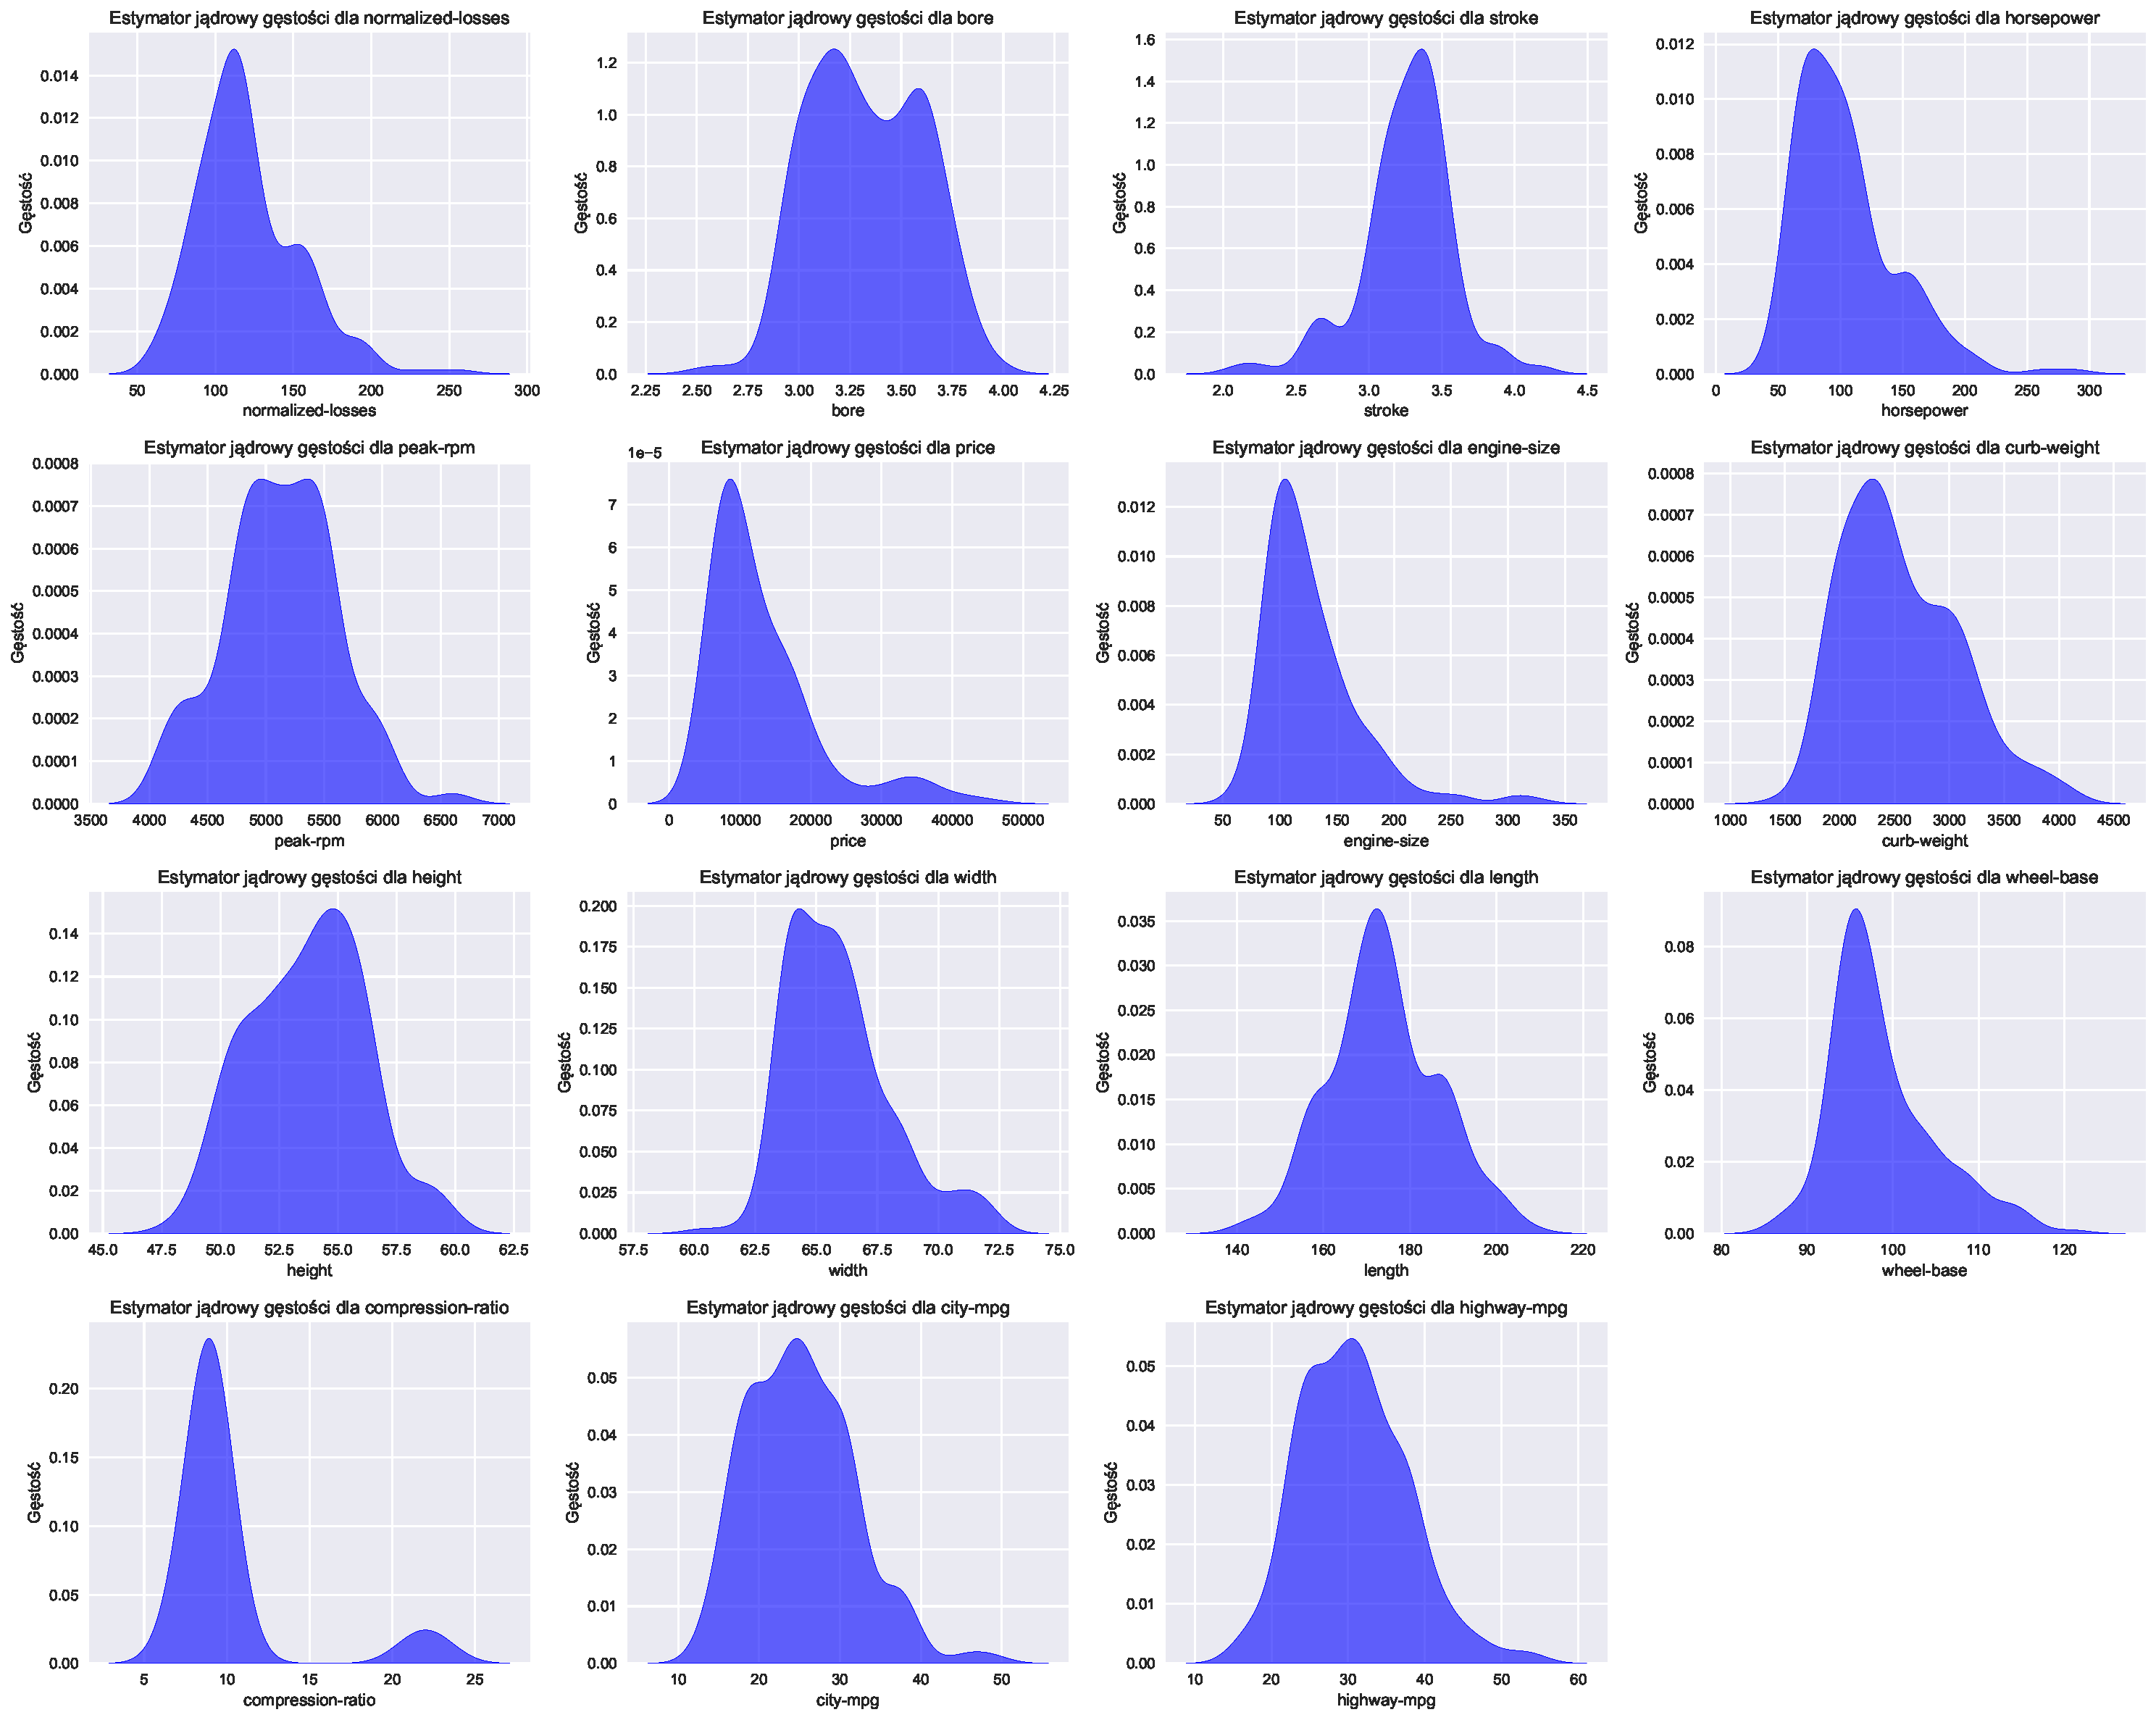
\includegraphics[width=0.95\textwidth]{all_kde_plots.pdf}
    \caption{Estymatory jądrowe gęstości dla wszystkich zmiennych ciągłych}
    \label{fig:all_kde_plots}
    \small\textit{Wizualizacja estymatorów jądrowych gęstości dla wszystkich zmiennych ciągłych. Widoczne są różne kształty rozkładów, od zbliżonych do normalnego, przez silnie asymetryczne, aż po charakterystyczny dwumodalny rozkład zmiennej \texttt{compression-ratio}.}
\end{figure}

\subsection{Analiza rozkładów zmiennych}

Estymacja jądrowa gęstości pozwoliła na zaobserwowanie następujących cech rozkładów:

\begin{itemize}
    \item Wiele zmiennych (\texttt{price}, \texttt{horsepower}, \texttt{engine-size}, \texttt{compression-ratio}) charakteryzuje się asymetrycznym rozkładem z długim ogonem po prawej stronie, co sugeruje obecność wartości odstających.
    
    \item Niektóre zmienne (\texttt{peak-rpm}, \texttt{height}, \texttt{width}) mają rozkład zbliżony do normalnego, skupiony wokół jednej dominującej wartości.
    
    \item Zmienna \texttt{compression-ratio} wykazuje rozkład dwumodalny, co może sugerować obecność dwóch różnych klas silników (np. benzynowe vs. wysokoprężne).
    
    \item Zmienne \texttt{city-mpg} oraz \texttt{highway-mpg} mają rozkłady przesunięte ku lewej, co oznacza, że większość samochodów ma umiarkowane zużycie paliwa, a tylko nieliczne cechują się bardzo wysoką efektywnością.
\end{itemize}

\subsection{Znaczenie analizy KDE}

Estymatory jądrowe gęstości pozwalają lepiej zrozumieć strukturę danych, wykryć potencjalne problemy oraz dobrać odpowiednie transformacje zmiennych. Analiza ta stanowi istotny etap przygotowawczy przed zastosowaniem algorytmów uczenia maszynowego lub budową modeli statystycznych.

\begin{figure}[H]
    \centering
    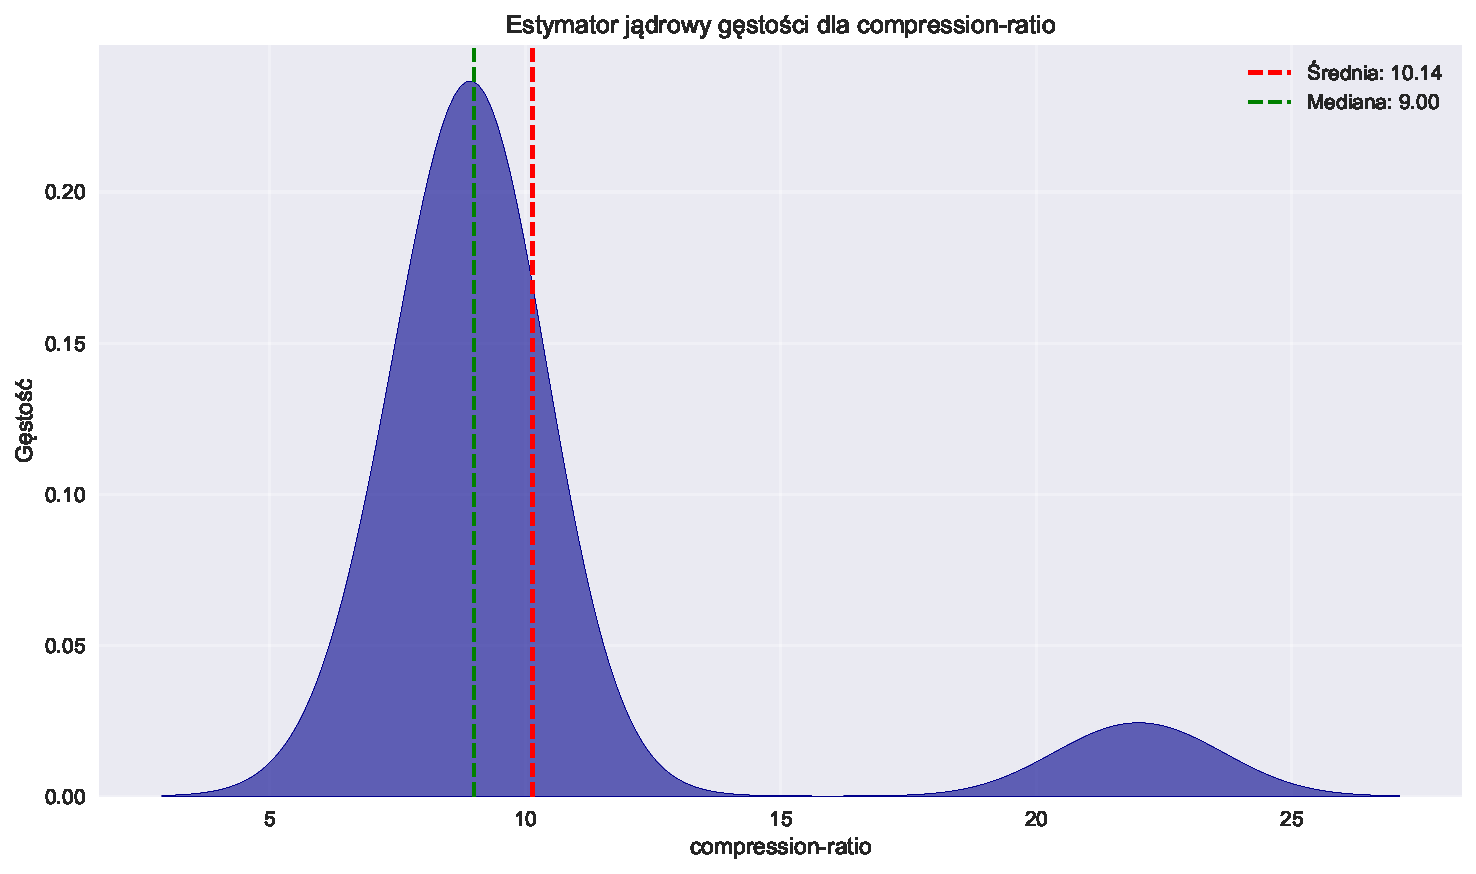
\includegraphics[width=0.75\textwidth]{kde_compression-ratio.pdf}
    \caption{Estymator jądrowy gęstości dla zmiennej compression-ratio}
    \label{fig:kde_compression_ratio}
    \small\textit{Wizualizacja estymacji jądrowej gęstości dla zmiennej compression-ratio, ukazująca charakterystyczny dwumodalny rozkład. Dwa wyraźne szczyty mogą wskazywać na różne kategorie silników.}
\end{figure}

\section{Podsumowanie i wnioski}

Przeprowadzona analiza statystyczna zbioru danych Automobile pozwoliła na poznanie kluczowych właściwości opisywanych zmiennych oraz relacji między nimi.

\subsection{Główne obserwacje}

\begin{itemize}
    \item Większość zmiennych nie podlega rozkładowi normalnemu, co potwierdziły zarówno wizualizacje, jak i formalne testy statystyczne.
    
    \item Zmienne cenowe i techniczne związane z mocą silnika (\texttt{price}, \texttt{horsepower}, \texttt{engine-size}) charakteryzują się silną asymetrią prawostronną, co wskazuje na istnienie niewielkiej liczby drogich, wysokowydajnych pojazdów.
    
    \item Zaobserwowano silne korelacje między zmiennymi technicznymi, zgodne z oczekiwaniami inżynieryjnymi (np. dodatnia korelacja między mocą a pojemnością silnika, ujemna korelacja między mocą a zużyciem paliwa).
    
    \item Metody bootstrapowe okazały się bardziej odpowiednie do estymacji przedziałowej dla zmiennych o asymetrycznych rozkładach, dostarczając przedziałów ufności lepiej dostosowanych do danych.
\end{itemize}

\kod{
# Zapisanie wszystkich wyników analiz do pliku
summary_text = """
PODSUMOWANIE ANALIZ STATYSTYCZNYCH - ZBIÓR DANYCH AUTOMOBILE

1. CHARAKTERYSTYKA DANYCH:
   - 205 instancji (samochodów)
   - 26 atrybutów (zmiennych)
   - Analizowane zmienne ciągłe: price, horsepower, engine-size, curb-weight, city-mpg, highway-mpg, etc.

2. GŁÓWNE WNIOSKI:
   - Większość zmiennych wykazuje odchylenie od rozkładu normalnego
   - Zmienne price, horsepower i engine-size charakteryzują się silną asymetrią prawostronną
   - Zaobserwowano silne, zgodne z intuicją korelacje między zmiennymi technicznymi
   - Metody bootstrapowe okazały się bardziej odpowiednie dla zmiennych o asymetrycznych rozkładach
   - Zmienna compression-ratio wykazuje charakterystyczny rozkład dwumodalny

3. IMPLIKACJE:
   - W analizach należy uwzględnić nienormalność rozkładów większości zmiennych
   - Przy modelowaniu zalecane są metody odporne na odstające wartości
   - Do estymacji przedziałowej lepiej stosować metody bootstrapowe niż klasyczne
"""

print(summary_text)
}{Podsumowanie przeprowadzonych analiz statystycznych}

\end{document}
